%% Based on canonical example (abntex2)
% pretextuais paginas
% mover capitulo 3 para introducao
% (a pensar) Mudar para ref. tipo abnt (sem numero)
% Deixar a rev. sis. como anexo
% referencias: et. al.
% referencias: links
% Titulos do capitulo 5
% referencias: and
% referencias em cada capitulo
% colocar resultados do ga no cap 5 (ate ~30).

\documentclass[oldfontcommands,12pt,openright,twoside,a4paper,brazil]{abntex2}
\usepackage{abntex2-ufam}
\bibstyle{apa}

%\usepackage{longtable}

% ---
% PACOTES
% ---

% ---
% Pacotes fundamentais 
% ---
\usepackage{cmap}				% Mapear caracteres especiais no PDF
\usepackage{lmodern}			% Usa a fonte Latin Modern			
\usepackage[T1]{fontenc}		% Selecao de codigos de fonte.
\usepackage[utf8]{inputenc}		% Codificacao do documento (conversão automática dos acentos)
\usepackage{lastpage}			% Usado pela Ficha catalográfica
\usepackage{indentfirst}		% Indenta o primeiro parágrafo de cada seção.
\usepackage{color}				% Controle das cores
\usepackage{graphicx}			% Inclusão de gráficos
\usepackage[final]{pdfpages}

\usepackage[table,xcdraw]{xcolor}

%\usepackage{enumerate}
\usepackage{enumitem}

% systematic review
\usepackage{lineno,hyperref}
%\biboptions{numbers,sort&compress}
\usepackage[version=0.96]{pgf}
\usepackage{tikz}
\usepackage[group-separator={,}]{siunitx}
\usepackage[caption=false]{subfig}
\usepackage{pdflscape}
\usetikzlibrary{automata,petri,calc,positioning,shapes.geometric,arrows,shapes,backgrounds}
\usepackage{threeparttable}
\usepackage{longtable}
\usepackage{threeparttablex,booktabs}
% ---
% ---

% ---
% Pacotes de citações
% ---
%\usepackage[hyperpageref]{backref}	 % Paginas com as citações na bibl
%\citebrackets[] 

% ---
% Pacotes do texto
% ---
%\usepackage{hyperref}
\usepackage{colortbl}
\usepackage{color}
\usepackage{amsmath}
\usepackage{breqn}
\usepackage{amsfonts}
\usepackage{amssymb}
\usepackage{url}
\usepackage{pgfgantt}
\usepackage{subfig}
\usepackage{relsize}

\usepackage[brazil]{babel}
\usepackage[fixlanguage]{babelbib}
\selectbiblanguage{brazil}

\usepackage{setspace}
\usepackage{pdflscape}

\usepackage{multirow} 
\usepackage[utf8]{inputenc}


\usepackage[ruled]{algorithm}
\usepackage{algorithmic}
\usepackage{pgfgantt}
\usepackage{epigraph}

%\usepackage[fixlanguage]{babelbib}
%\selectbiblanguage{brazil}
%\bibliographystyle{babplain-lf}

\newcommand*\rot{\rotatebox{90}}
\newcolumntype{L}{>{\centering\arraybackslash}m{11.5cm}}

\newcolumntype{A}{>{\centering\arraybackslash}m{4.0cm}}

\newcolumntype{M}{>{\arraybackslash}m{11.5cm}}
%% Novo estilo
\makepagestyle{estilo_pretextual} %%% escolha um nome
  \makeevenhead{estilo_pretextual}{}{}{\ABNTEXfontereduzida \textbf \thepage}
  \makeoddhead{estilo_pretextual}{}{}{\ABNTEXfontereduzida \textbf \thepage}

%% Customiza comando \pretextual
\renewcommand{\pretextual}{
  \pagenumbering{roman} %%% ou \pagenumbering{Roman}
  \aliaspagestyle{chapter}{estilo_pretextual}% customizing chapter pagestyle
  \pagestyle{estilo_pretextual}
  \aliaspagestyle{cleared}{empty}
  \aliaspagestyle{part}{estilo_pretextual}
}

% ---
% Ajusta a marca \textual para que a numeração volte a ser arábica
% nos elementos textuais
\let\oldtextual\textual        % copia o comando \textual anterior para \oldtextual
\renewcommand{\textual}{%
  \oldtextual%
  \pagenumbering{arabic} % volta à numeração arábica
}
% ---

\selectlanguage{brazil}

%% ABNTEX
%\titulo{Reconhecimento de Emoção por Expressão Facial Utilizando Redes Neurais de Convolução}
\titulo{Uma Abordagem para Reconhecimento de Emoção por Expressão Facial baseada em Redes Neurais de Convolução}
\autor{Anderson Araújo da Cruz}
\local{Manaus -- AM}
\data{Agosto, 2018}
\orientador{Raimundo da Silva Barreto, D.Sc.}
\instituicao{%
  Universidade Federal do Amazonas -- UFAM
  \par
  Instituto de Computação  -- IComp
  \par
  Programa de Pós-Graduação em Informática -- PPGI}
\tipotrabalho{Thesis (Doctoral)}
\preambulo{Texto de qualificação submetido ao Programa de Pós-Graduação em Informática do Instituto de Computação da Universidade Federal do Amazonas para obtenção de pré-requisito para o título de mestrado \textit{stricto sensu}.}

\membroum{José Reginaldo Hughes Carvalho, D.Sc.}
\membrodois{Daniel Lins da Silva, D.Sc.}

% ---
% Configurações de aparência do PDF final

% alterando o aspecto da cor azul
\definecolor{blue}{RGB}{41,5,195}

% informações do PDF
\makeatletter
\hypersetup{
     	%pagebackref=true,
		pdftitle={\@title}, 
		pdfauthor={\@author},
    	pdfsubject={\imprimirpreambulo},
	    pdfcreator={LaTeX with abnTeX2},
		pdfkeywords={abnt}{latex}{abntex}{abntex2}{trabalho acadêmico}, 
		colorlinks=true,       		% false: boxed links; true: colored links
    	linkcolor=blue,          	% color of internal links
    	citecolor=blue,        		% color of links to bibliography
    	filecolor=magenta,      		% color of file links
		urlcolor=blue,
		bookmarksdepth=4
}
\makeatother
% --- 

% --- 
% Espaçamentos entre linhas e parágrafos 
% --- 

% O tamanho do parágrafo é dado por:
\setlength{\parindent}{1.3cm}

% Controle do espaçamento entre um parágrafo e outro:
\setlength{\parskip}{0.2cm}  % tente também \onelineskip

% ---
% compila o indice
% ---
\makeindex
%% ABNTEX

%% Hyphenization mistakes
\hyphenation{analy-sis}
\hyphenation{analy-ses}

\begin{document}
\selectlanguage{brazil} %Required for translation

% Retira espaço extra obsoleto entre as frases.
\frenchspacing 

% ----------------------------------------------------------
% ELEMENTOS PRÉ-TEXTUAIS
% ----------------------------------------------------------
\pretextual

% ---
% Capa
% ---
\imprimircapa
% ---

% ---
% Folha de rosto
% (o * indica que haverá a ficha bibliográfica)
% ---
% Na UFAM, a ficha catalográfica é impressa na biblioteca
\imprimirfolhaderosto*
% ---

% ---
% Inserir a ficha bibliografica
% ---

% Isto é um exemplo de Ficha Catalográfica, ou ``Dados internacionais de
% catalogação-na-publicação''. Você pode utilizar este modelo como referência. 
% Porém, provavelmente a biblioteca da sua universidade lhe fornecerá um PDF
% com a ficha catalográfica definitiva após a defesa do trabalho. Quando estiver
% com o documento, salve-o como PDF no diretório do seu projeto e substitua todo
% o conteúdo de implementação deste arquivo pelo comando abaixo:

%\begin{fichacatalografica}
    % 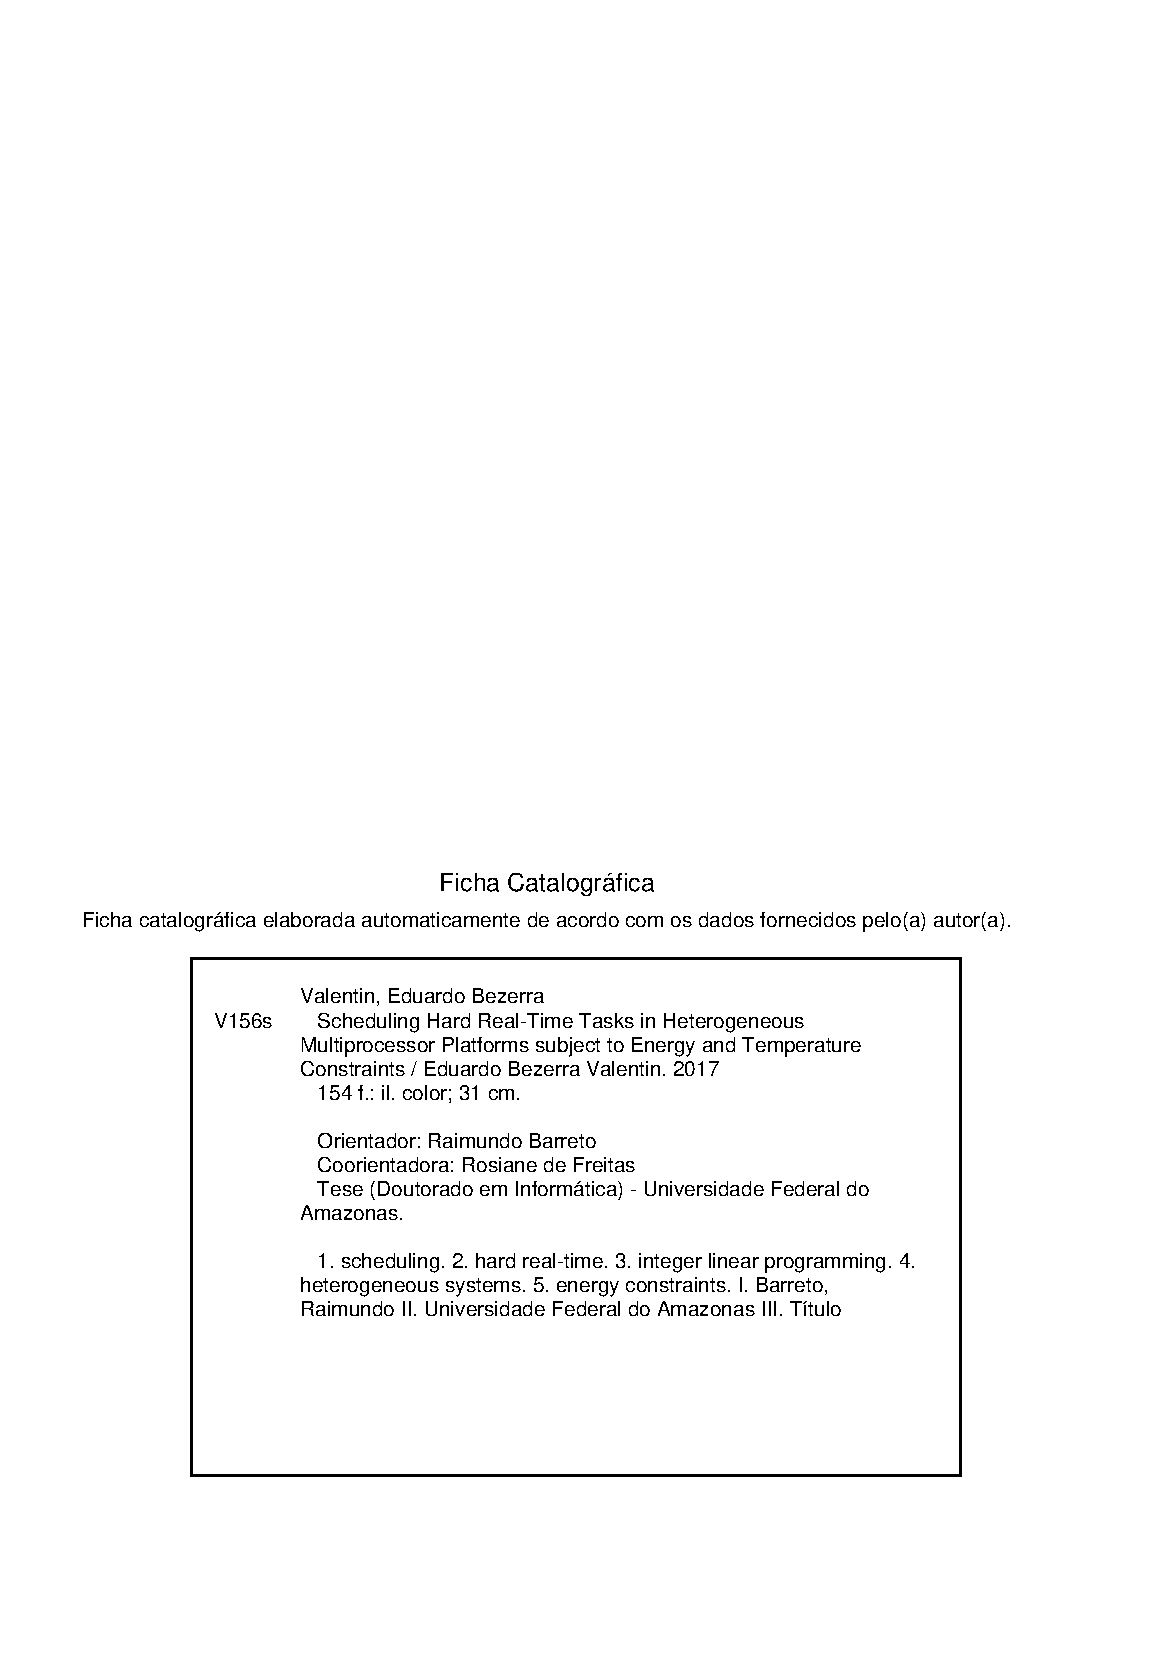
\includepdf{FichaCatalografica.pdf}
%\end{fichacatalografica}
% ---

% ---
% Inserir folha de aprovação
% ---

% Isto é um exemplo de Folha de aprovação, elemento obrigatório da NBR
% 14724/2011 (seção 4.2.1.3). Você pode utilizar este modelo até a aprovação
% do trabalho. Após isso, substitua todo o conteúdo deste arquivo por uma
% imagem da página assinada pela banca com o comando abaixo:
%
% \includepdf{folhadeaprovacao_final.pdf}
%


%FOLHA DE APROVACAO
\imprimirfolhadeaprovacao

% ---
% Dedicatória
% ---
%\begin{dedicatoria}
%   \vspace*{\fill}
%   \centering
%   \noindent
%   \textit{To all computer engineers who\\
%   might be using a scope to measure voltage wave form.} \vspace*{\fill}
%\end{dedicatoria}
% ---

% ---
% Agradecimentos
% ---
%\begin{agradecimentos}[Acknowledgments]

%\epigraph{``And let steadfastness have its full effect, 
%that you may be perfect and complete, lacking in nothing.''}{\textit{James 1:4}}

%This has been a difficult, but joyful, journey which I have had God's help to this very day. I know that on every obstacle that I thought too hard to cross, He has given me strength and perseverance. Therefore, I thank God, for blessing me with the patience, the intelligence, and the ability to complete this work. My life belongs to Him.

%I want to say thank you to my wife, Belisa Magalhães, Bela, for the true love. She was the one to first believe and trigger the motivation in me to start this journey. Thanks to Bela for the discussions about research challenges and researcher's life and role. Thanks for listening about my research, even when the subject was not of interest. For sure, without her support, patience, and care I would not completed this work. To my kids, Ed and Estela, thanks for giving up the time with Dad, so he could work. Many thanks to my family, in special to my mother, Fátima, for her love, care, attention, and understanding; to my father,  Edson (\emph{in memorian}) and my brothers, Fábio and Milton (\emph{in memorian}), for their valuable contribution to my education.

%Many thanks to my advisor, professor Raimundo Barreto. One would say I could have done this work anywhere I pleased, and I chose to follow an example of steadfastness. Thanks for the understanding, support, guidance, focus, invested time, and believing in my work. Thanks for sharing with me a little of the challenges of conducting successful research in the Amazon region of Brazil. Perhaps, one day, I too will be an eagle.

%I wish many thanks to my co-advisor, professor Rosiane de Freitas. Thanks for the patience to walk me through the world of combinatorial optimization. Thanks for always having insights and showing me different perspectives of the same problem.

%Thanks to all colleagues from GISE research group. Thanks to all friends, staff members, and professors at ICOMP/UFAM. Thanks for the partial financial support provided by SOBRAPO,  FAPEAM, and CAPES.

%\end{agradecimentos}

% ---

% ---
% Epígrafe
% ---
\begin{epigrafe}
    \vspace*{\fill}
	\begin{flushright}
		\textit{``Os loucos que acham que podem mudar o mundo,\\
						são os que efetivamente o fazem''}
						
		Comercial Apple - ``Pense Diferente'', 1997
	\end{flushright}

%    \vspace*{\fill}
%\epigraph{``Computers may be thought of as engines for 
%transforming free energy into waste heat 
% and mathematical work''}{\textit{Charles H. Bennett, 1981}}
\end{epigrafe}
% ---

% ---
% RESUMOS
% ---

% resumo em inglês
\begin{resumo}
Neste trabalho, uma abordagem é apresentada para o reconhecimento de emoção por meio da expressão facial utilizando redes neurais de convolução. Esta abordagem consiste em reconhecer emoções por meio de processamento digital de imagens e realizar diversas transformações na imagem com a finalidade de classificar as emoções. Esta proposta contempla problemas clássicos na classificação de imagens, como problemas de iluminação do ambiente e rotações do objeto principal, neste caso, a face. Uma revisão sistemática da literatura foi conduzida para mapeamento da área e a obtenção de uma visão geral. Foram descobertas as principais arquiteturas de redes neurais de convolução, e percebeu-se que ainda não há um direcionamento para qual caso é melhor optar por uma arquitetura ou outra e também a ausência de experimentos justos que possam verificar qual arquitetura alcança maior taxa de reconhecimento. Diversas aplicações foram localizadas na literatura, desde aplicações em interação humano-computador e humano-robô a cuidados com a saúde, entretanto, estas aplicações ainda não estão sendo usadas na prática, são apenas especulações, com potencial de fato serem utilizadas na próxima década. Apesar das redes neurais de convolução possuírem transformações de pré-processamento embutidas na própria arquitetura, o uso de pré-processamento na imagem antes da inserção na rede tem se mostrado eficaz e aumentado a taxa de reconhecimento. Isto evidencia a dificuldade de reconhecer emoções em expressão facial, pois geralmente a rede neural de convolução tem resolvido muitos problemas sem qualquer pré-processamento externo com acurácia elevada. O primeiro resultado parcial consistiu na utilização de uma API externa para reconhecer emoções, no qual monitorava estudantes em tempo real, enquanto estavam respondendo um simulado da prova do Exame Nacional do Ensino Médio (ENEM). Posteriormente, foram cruzadas as emoções detectadas com o desempenho no teste. Diante disso, esta prova de conceito norteou o desenvolvimento preliminar desta proposta gerando um reconhecedor de emoções baseado na arquitetura AlexNet, que foi treinada por mais de 28 mil imagens.  


%Foi verificado que o uso de pré-processamento na imagem antes da inserção na rede neural de convolução melhora a taxa de reconhecimento. Isto evidencia a dificuldade de reconhecer emoções em expressão facial, pois redes neurais de convolução são muito poderosas e possuem transformações de pré-processamento embutidas na própria arquitetura. 



   \vspace{\onelineskip}
 
   \noindent 
   \textbf{Palavras-chaves}: Reconhecimento de Emoção, Expressão Facial, Redes Neurais de Convolução.
\end{resumo}


% ---
% inserir lista de ilustrações
% ---
\pdfbookmark[0]{\listfigurename}{lof}
\listoffigures*
\cleardoublepage
% ---

% ---
% inserir lista de tabelas
% ---
\pdfbookmark[0]{\listtablename}{lot}
\listoftables*
\cleardoublepage
% ---

% ---
% inserir lista de abreviaturas e siglas
% ---
\begin{siglas}
  \item[RNC] Rede Neural de Convolução.
  \item[ILSVRC] ImageNet Large Scale Visual Recognition Challenge.
\end{siglas}
% ---

% ---
% inserir lista de símbolos
% ---
%\begin{simbolos}
%  \item[$D_i$] Deadline of $ \tau_i $.
%  \item[$Lp$] DVFS Switching Latency.
%\end{simbolos}
% ---

% ---
% inserir lista de tabelas
% ---
%\pdfbookmark[0]{\listalgorithmname}{loa}
%\listofalgorithms
%\cleardoublepage

% ---
% inserir o sumario
% ---
\pdfbookmark[0]{\contentsname}{toc}
\tableofcontents*
\cleardoublepage
% ---

% ----------------------------------------------------------
% ELEMENTOS TEXTUAIS
% ----------------------------------------------------------
\textual

\chapter{Introdução}\label{sec:introducao}

\section{Contexto}
Há décadas a comunidade científica tem se interessado no reconhecimento de emoções. As diversas maneiras de expressar as emoções humanas têm sido investigadas, tais como sinais fisiológicos, textos, envio de \textit{emoticons}, dispositivo padrão de entrada de dados (e.g. teclado e mouse), voz e as expressões faciais. Esta última surgiu pelas anotações de \cite{darwin1965expression} e experiências de \cite{ekman1994}, que perceberam que todas as culturas emitem emoção pela expressão facial acreditando na existência de um grupo de emoções básicas (raiva, felicidade, tristeza, desprezo, medo e surpresa) que possuem a mesma expressão facial independente da cultura dos indivíduos. Apesar de tantos anos de pesquisa, a comunidade continua interessada neste assunto, pois reconhecer emoção tem sido desafiador, além de ser um campo promissor para a interação humano-computador e humano-robô. Ainda é considerado um problema em aberto, inclusive com a realização de concursos com premiação, como foi o caso do ICML'2013 e anualmente como o EmotiW dos anos de 2014 a 2017.

O progresso da área de aprendizado profundo ocasionou o surgimento de diversas técnicas poderosas de reconhecimento de padrões, gerando grande destaque para as redes neurais de convolução, que foram projetadas para processamento e classificação de imagem. As redes neurais de convolução têm sido bastante populares e utilizadas em diversos contextos dominando amplamente os trabalhos realizados pela comunidade ultimamente. Possibilitando, inclusive, o reconhecimento automático de emoção por meio da expressão facial, sendo que tal reconhecimento está próximo do que um humano reconheceria \citep{kim2016fusing}. Estes resultados expressivos têm motivado pesquisadores a continuar aprimorando estas técnicas e a expressão facial tem se tornado uma abordagem eficaz para reconhecer emoções, pois não é uma abordagem intrusiva de coleta de dados quando comparada aos sensores fisiológicos. Tais sensores não são uma computação ubíqua que resulta no incomodo do usuário quando seus sinais fisiológicos são monitorados, além disso, a expressão facial possui a facilidade de ser obtida em uma captura de imagem devido a popularidade de dispositivos que possuem câmeras fotográficas \citep{cruz2017framework}.

\section{Motivação}
O reconhecimento de emoção tem aplicação em muitas áreas. Destacamos alguns campos promissores. Na educação, por exemplo, segundo \cite{jaques2013ambientes}, estudantes durante o seu processo de aprendizagem emitem constantemente diversas emoções. Além disso, sistemas educacionais como Ambientes Virtuais de Aprendizagem (AVA) e Sistemas de Tutores Inteligentes (STI) podem monitorar as emoções durante a interação com uma plataforma educacional em uma aula, por exemplo, para fornecer \textit{feedback} personalizado para o estudante recomendando objetos de aprendizagem apropriados para aquele estado emocional e até mesmo, realizar ações que estimulem emoções positivas a fim de motivar os estudantes quando estes estiverem em um estado negativo. Outra área de aplicação para utilizar o reconhecimento de emoção é em realidade virtual. Segundo \cite{riva2007affective}, a realidade virtual pode estimular propositalmente emoções permitindo maior imersão do usuário à aplicação. Desta forma, o reconhecimento de emoção pode medir o quão efetivo é o método de estimular emoções ao usuário e, caso não seja satisfatório, o método de estímulo de emoção pode ser alterado. Para \cite{li2015deep}, o reconhecimento de emoção pode auxiliar na construção de tecnologias assistivas para deficientes visuais que, quando possuem elevado grau de deficiência, apresentam dificuldades em reconhecer emoções na interação interpessoal. Em geral, é possível aplicar o reconhecimento de emoção na interação humano computador \citep{chen2017convolution,wen2017ensemble,liu2016facial, barsoum2016training}, e interação humano robô \citep{shin2016baseline,jung2015development}, criando a expectativa de que computadores do futuro possam reconhecer a emoção do usuário e realizar algum procedimento que ocasione maior aproximação entre homem e máquina.    

\section{Definição do Problema}\label{sec:problema}
Trata-se de um problema de classificação de imagem digital no qual há uma imagem $\omega$ formada por um conjunto de \textit{pixels} (RGB) $\alpha$ pertencente a um conjunto de classes $\sigma$ = \{neutralidade, raiva, felicidade, tristeza, desprezo, medo e surpresa\}, que são as emoções básicas definidas por \citep{ekman1994}, tal que haja uma função $\phi$ que saiba mapear $\omega$ por meio de $\alpha$ para $\sigma$.  

Embora existam trabalhos que classifiquem emoções em imagens \citep{kim2016fusing, yu2016customized,barsoum2016training}, pouca atenção tem sido dada aos problemas clássicos em imagens como: (i) ausência de iluminação no ambiente; (ii) rotação do objeto principal, neste caso a face, e (iii) escala do objeto principal (face). Abordagens que tratam estes problemas em imagens são mais apropriadas para o uso em cenários reais no qual a exigência  para classificação é maior devido as condições adversas do ambiente e pelas diferentes variações das características da face humana. 

O problema considerado neste trabalho pode ser expresso na seguinte questão: \textit{Como aprimorar os métodos de reconhecimento de emoções por meio da expressão facial a fim de permitir a classificação independente das características do ambiente e de indivíduos para o alcance de maior generalização?} 

\section{Objetivos}

\subsection{Objetivo Geral}
Propor um método para reconhecer emoção humana por expressão facial para classificar emoções básicas em múltiplas faces de uma imagem e comparar a eficácia em cenários de uso real.
%Desenvolver um reconhecedor de emoção humana por expressão facial utilizando redes neurais de convolução para classificar as emoções básicas em múltiplas faces de uma imagem, e comparar a sua eficácia em cenários de uso real.

\subsection{Objetivos Específicos}
\begin{itemize}
 %\item Gerar um módulo de pré-processamento para eliminação de ruídos;
 %\item Propor um detector de face para recortar as diversas faces em uma imagem;
 %\item Implementar uma rede neural de convolução para em uma imagem para realizar extração de características, redução de dimensionalidade e classificação;
 \item Propor técnicas de eliminação de ruídos e detecção com recorte das diversas faces de uma imagem;
 \item Classificar cada face detectada separadamente estimando a probabilidade para cada emoção básica;
 \item Avaliar experimentalmente a solução proposta visando a comparação da eficácia.
\end{itemize}

\section{Hipótese}
As emoções básicas emitidas por expressão facial podem ser reconhecidas por uma rede neural de convolução, desde que esteja treinada e validada por instâncias representativas do problema (veja Seção \ref{sec:problema}). Este trabalho apoia-se na combinação entre uma rede neural de convolução profunda com a eliminação de ruídos da imagem por meio da utilização de técnicas de pré-processamento. A eliminação de ruídos antes da inserção da imagem na rede neural de convolução promove maior acurácia na classificação, aumento da generalização e do aprendizado para o reconhecimento de emoção em diferentes ambientes e variações da face humana.  

%Se utilizar redes neurais de convolução juntamente com técnicas de pré-processamento, aplicando transformações na imagem, como escala de cinza, filtros e redimensionamento da imagem e, realizar o mapeamento das formas presentes na imagem, como pontos relevantes da face que se alteram quando há emissão de uma determinada emoção, então, torna-se possível a classificação de emoções do usuário por meio das expressões faciais, realizando processamento digital de imagens a partir do treinamento da rede com a imagem pré-processada, focalizando na extração de características relevantes para a separação das classes. 

\section{Abordagem Proposta}\label{sec:abordagemproposta}

\subsection{Visão Geral da Solução Proposta}
Uma visão geral da solução proposta é apresentada na Figura \ref{fig:arquitetura}. É uma solução que está direcionada para o reconhecimento de emoção por expressão facial no qual a abordagem recebe uma imagem qualquer que pode ter sido capturada por algum dispositivo de monitoramento que contém câmera fotográfica (e.g. smartphone, notebook, televisão e outros). Toda  fotografia capturada pelo dispositivo de monitoramento é salva em um repositório de entrada de dados. Este repositório é consultado para obter uma imagem e enviá-la para a classificação. No processo de classificação é verificada a existência de uma face na imagem e, caso não exista, é encerrada a execução, pois é uma imagem que não contém uma face, logo, não existe uma expressão facial para classificar e novamente é consultado o repositório de entrada de dados para se obter uma nova imagem. Caso exista uma face, uma função para recortá-la é chamada. Este procedimento é valoroso por dois aspectos: o primeiro por excluir o \textit{background} da imagem, pois assim o classificador não necessita aprender a diferenciar o que é face e \textit{background}, e o segundo é pela possibilidade de haver múltiplas faces na imagem realizando a classificação de cada face individualmente, reduzindo a complexidade do problema, pois é mais fácil classificar uma face por vez do que várias ao mesmo tempo. Posteriormente, a face recortada é enviada a um conjunto de filtros de pré-processamento que por sua vez operam sobre a imagem para eliminação de ruídos. Finalmente, a imagem pré-processada é enviada a uma rede neural de convolução para a classificação. Esta técnica pode ter uma característica em particular que é interessante: em vez de retornar à classe a que a expressão facial (ou uma instância) pertence, pode retornar às estimativas de probabilidade para cada classe da expressão facial (e.g. neutralidade: 0.95, felicidade: 0.025, medo: 0.025,...) possuindo assim uma propriedade em que a soma das probabilidades de todas as classes é igual a 1 e a classificação seria a maior probabilidade estimada (neutralidade com 95\% de certeza), e as estimativas de probabilidade são salvas em um repositório de saída de dados. O processo anteriormente descrito deve ser repetido enquanto houver faces para classificar, isto é, quando uma imagem há múltiplas faces, e cada face é classificada uma por vez.

\subsection{Computação embarcada e em nuvem}
Esta proposta visa fornecer soluções para reconhecimento de emoção que contempla dois tipos de computação: em nuvem e embarcada. Tais computações estão em alta na academia, indústria e mercado. A primeira pelo crescimento da internet havendo bilhões de dispositivos conectados e a evolução da infraestrutura com aumento considerável de recursos computacionais e velocidade de conexão. A segunda pela explosão de dispositivos embarcados presentes em nosso cotiano. Além disso, os dispositivos embarcados de hoje tem uma autonomia energética periódica, hardware semelhante a desktops, sistemas operacionais e sensores embutidos, formando um dispositivo independente e poderoso. Há no mercado smartphones e smartwatches com processadores octa-core e dual-core respectivamente, com a memória RAM chegando a 8GB, e até mesmo com placas de vídeos embutidas para aceleração de computação.        

A computação em nuvem hospedaria o melhor modelo gerado a partir das arquiteturas AlexNet, VGGNet, GoogLeNet e Residuais, considerando métricas de avaliação de desempenho como precisão, revocação e f1-score. Apesar de que o melhor modelo possa exigir elevada utilização de recursos computacionais por ser uma rede neural profunda, entende-se que um serviço em nuvem possuiria um hardware robusto capaz de suportar a demanda da rede neural de convolucão. Visto que estamos no boom da computação cognitiva, isto é, a capacidade de computadores pensarem como humanos. A ideia de ter um reconhecedor de emoções em um serviço em nuvem é para quaisquer aplicação, independente de qual linguagem de programação foi implementada ou em qual sistema operacional está sendo executada, enviar imagens via padrão REST com intuito de receber a classificação das imagens com as emoções detectadas.    

A computação embarcada consiste na rede neural de convolução baseada na arquitetura MobileNet funcionar nativamente em um dispositivo embarcado. Essa arquitetura foi projetada para consumir menos recursos computacionais com o compromisso de perder o mínimo de precisão, sendo ideal para dispositivos embarcados que dispõe de menos recursos computacionais. Inclusive podendo funcionar nativamente no sistema operacional Android que é amplamente usado por \textit{smartphones}, \textit{smartwatches} e \textit{tablets}. Além disso, a arquitetura MobileNet pode ser também embutida em placas de desenvolvimento como Raspberry, Nvidia Jetson, Drones e outras.  

Vale destacar que as maiores taxas de ocupação de recursos computacional de uma rede neural de convolução estão na fase de treinamento, isto é, durante a geração do modelo. E a fase de classificação exige menores taxas de ocupação de hardware, pois o principal procedimento que demanda recursos computacionais consiste em carregar o modelo na memória. Quando uma imagem é enviada para classificação, considerando que o modelo está carregado na memória, a rede neural opera sobre a imagem aplicando os pesos advindos do modelo. Diferentemente da fase de treinamento que exige muito processamento, pois é executado o algoritmo de otimização gradiente descendente para minimizar a função de perda realizando uma alta quantidade de cálculos vetoriais.   


\begin{figure}
\centering
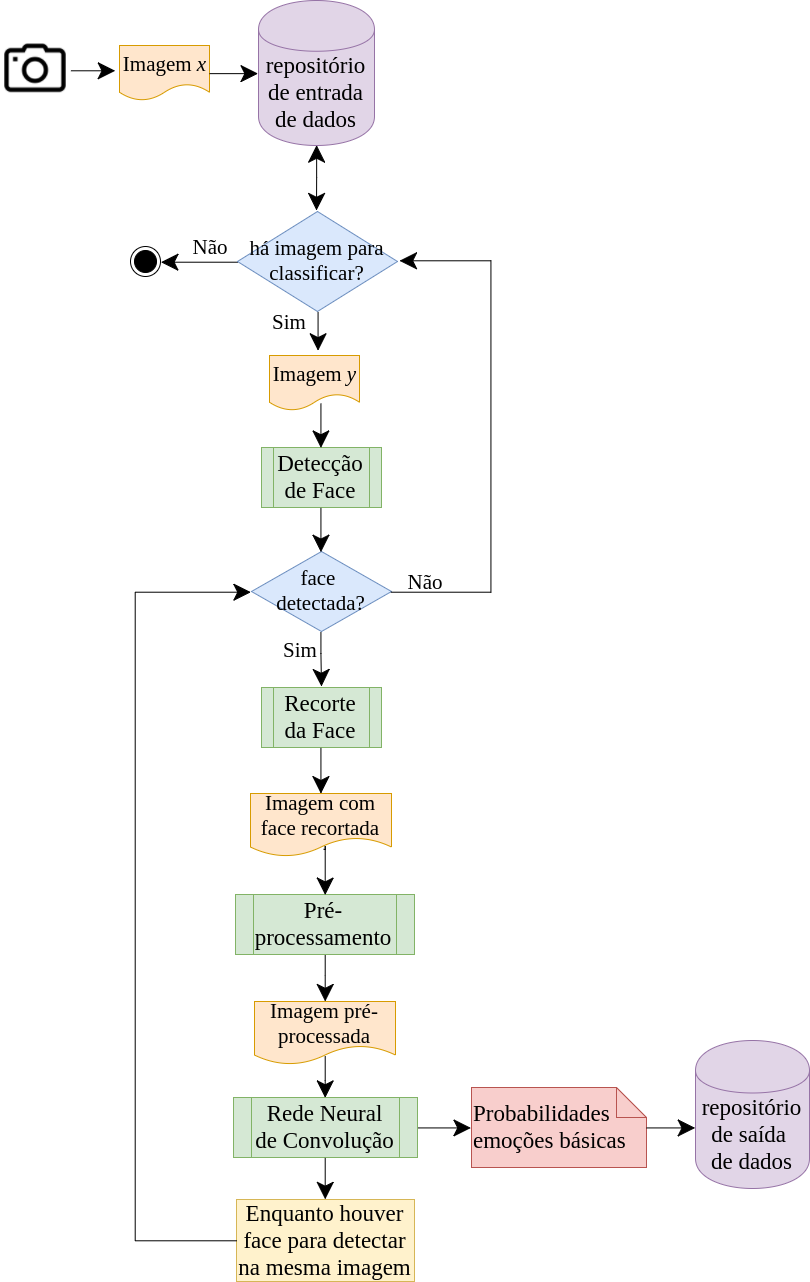
\includegraphics[scale=0.45]{figuras/arquitetura.png}
\caption{Solução Proposta}
\label{fig:arquitetura}
\end{figure}

\section{Organização do Trabalho}
Este trabalho está dividido nos capítulos a seguir. O Capítulo \ref{sec:conceitos} aborda os conceitos e definições necessários para o entendimento deste trabalho. O Capítulo \ref{sec:relacionados} analisa os trabalhos relacionados. O Capítulo \ref{sec:abordagemproposta} apresenta a abordagem proposta. O Capítulo \ref{sec:resultados} discute os resultados parciais obtidos. O Capítulo \ref{sec:cronograma} descreve o cronograma e detalha as atividades a serem realizadas enquanto o Capítulo \ref{sec:conclusao} enfatiza as considerações finais, limitações do trabalhos e os trabalhos futuros.

\chapter{Referencial Teórico}\label{sec:conceitos}
Neste capítulo são introduzidos os conceitos necessários para o entendimento deste trabalho e está organizado da seguinte forma. A Seção \ref{sec:recemo} define o que é o reconhecimento de emoção e os tipos de reconhecimento. A Seção \ref{sec:expfacia} fundamenta a expressão facial emocional e mostra as expressões básicas existentes. A Seção \ref{sec:apm} conceitua a área de aprendizagem de máquina. A Seção \ref{sec:pci} apresenta o processo de classificação de imagem. A Seção \ref{sec:tecnic} revisa as técnicas de pré-processamento que são utilizadas para eliminação de ruídos de uma imagem. As Seções \ref{sec:rna} e \ref{sec:rnc} conceituam os aspectos básicos das redes neurais artificiais e das redes neurais de convolução, respectivamente. A Seção \ref{sec:arc} descreve as arquiteturas de redes neurais de convolução utilizadas por este trabalho. A Seção \ref{sec:metavalclass} retrata as principais métricas para avaliar classificadores e para concluir a Seção \ref{sec:considf} faz um resumo acerca deste capítulo.   

\section{Reconhecimento de Emoção}\label{sec:recemo}
As emoções podem ser definidas como breves e intensas e são disparadas pela avaliação de um evento \citep{scherer2000psychological}. O reconhecimento de emoção tem sido explorado há algumas décadas e as emoções que tem sido frequentemente investigadas são as básicas como a raiva, alegria, tristeza, desgosto, medo e surpresa \citep{ekman1994}. Com objetivo de reconhecer emoção, os pesquisadores têm utilizado comumente as técnicas de reconhecimento de padrões, que por sua vez podem encontrar as características que são importantes para diferenciar as emoções, isto é, a busca pelo padrão relevante de uma entrada de dados, por exemplo uma imagem contendo uma expressão facial, de modo que a técnica consiga diferenciar a felicidade de neutralidade. Além disso, a comunidade tem gerado várias heurísticas para reconhecer emoções, entretanto com emprego somente em ambientes muito controlados. 

É possível reconhecer as emoções por diversas formas \citep{nasoz2004emotion}: (i) sensores capturando os sinais fisiológicos; (ii) análise de expressões faciais; (iii) análise da variação da fala por microfone; (iv) movimento corporal por meio da captura de dados por dispositivos padrões de entrada (i.e. mouse e teclado) e (v) análise do texto ao escrever uma opinião.

Este trabalho está limitado ao uso de expressões faciais para o reconhecimento de emoção devido às justificativas a seguir: (i) a popularidade de dispositivos que possuem câmeras fotográficas (e.g. smartphone, tablet, smart TV e notebook) facilitam a captura da expressão facial do usuário; (ii) a evolução das técnicas de classificação de imagens que estão alcançando a taxa de reconhecimento a nível humano e (iii) por não causar qualquer intrusão ao usuário, pois fotografias da expressão facial podem ser capturadas dentro do cotidiano das pessoas, não causa incômodo, não necessita o uso de instrumentos especiais, além de ser imperceptível aos usuários.

\section{Expressão Facial Emocional}\label{sec:expfacia}
\cite{darwin1965expression} verificou que fenômenos emocionais idênticos, principalmente relacionados as expressões faciais, podiam ser encontrados em diferentes culturas. Posteriormente, o trabalho de \cite{ekman1994} apontou a existência de um conjunto de expressões faciais universais que representam as mesmas emoções em diferentes culturas e estão exemplificadas na Figura \ref{fig:facesbasicas}. Essas expressões faciais universais pertencem ao grupo das emoções básicas, portanto é possível reconhecer as seguintes emoções por expressão facial: raiva, alegria, tristeza, desgosto, medo e surpresa. Cada emoção que é emitida por um indivíduo possui a sua própria movimentação muscular facial, sendo assim, há a caracterização de vários padrões que são chamados de unidades de ação, como o movimento da sobrancelha, dos olhos fechando, ao levantar as bochechas e entre outros \citep{ekman1977facial}. As unidades de ação são os padrões relevantes para diferenciar cada tipo de emoção. 

\begin{figure}
\centering
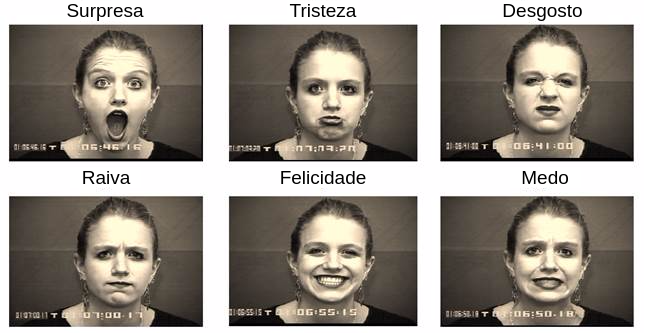
\includegraphics[scale=0.7]{figuras/facesbasicas.png}
\caption{Expressão facial emocional}
\label{fig:facesbasicas}
\end{figure}

\section{Aprendizagem de Máquina}\label{sec:apm}
Com intuito de criar sistemas que possuem a capacidade de reconhecer emoção de forma automática é muito comum o emprego de técnicas de aprendizagem de máquina, que é um ramo da inteligência artificial em que máquinas aprendem a partir de uma experiência e são habilitadas para reconhecer padrões. Uma definição de aprendizagem de máquina foi dada por \cite{alpaydin2014introduction}: \emph{“É a programação de computadores para otimizar um critério de desempenho usando dados de exemplo ou experiência passada”}. Na prática, isto pode ser entendido como a existência de um modelo definido com alguns parâmetros, no qual a ação de aprender consiste na execução de uma função de otimização, cujos parâmetros do modelo são otimizados, a partir dos dados de treinamento ou experiência passada. O modelo pode ser preditivo, para fazer previsões do futuro; descritivo, para obter conhecimento dos dados realizando a classificação; ou ambos.

Em aprendizagem de máquina, se as instâncias são conhecidas, isto é,  cada  instância possui o seu rótulo, então o aprendizado é supervisionado.  Caso contrário, se as instâncias são desconhecidas, a aprendizagem é não supervisionada. Neste trabalho, o aprendizado utilizado é o supervisionado no qual os métodos possuem uma fase de treinamento e outra de teste. A primeira consiste na utilização de um conjunto de características com instâncias previamente rotuladas, também conhecido como base de treino, com objetivo de encontrar padrões nos exemplos e, assim, produzir um modelo para armazenar o aprendizado. Por fim, na fase de teste, o algoritmo deve classificar dados desconhecidos, por meio da base de teste, a partir dos padrões encontrados na fase anterior e mensurar o desempenho obtido. Além disso, o modelo gerado pode ser testado por outra base chamada de validação para averiguar com mais confiança que não há aprendizagem viciosa. Caso o desempenho esteja satisfatório o método está apto para a produção, senão deve voltar para fase de treinamento \citep{kotsiantis2007supervised, geron2017hands}.

\section{Processo de Classificação de Imagem}\label{sec:pci}
Nos problemas de classificação de imagem, quando a abordagem é por meio da aprendizagem de máquina, geralmente é seguido o processo: (i) a etapa inicial consiste em uma fase de pré-processamento em que são aplicadas várias técnicas com a intenção de eliminar o ruído da imagem, resultando em sua melhora considerável para as fases posteriores; (ii) a etapa de extração de característica foca em destacar ou retirar as principais formas da imagem que são importantes para a separação das classes e (iii) as características extraídas são enviadas para um classificador determinar qual a classe que a imagem pertence.

\section{Técnicas para pré-processamento de imagens em reconhecimento de emoção por expressão facial}\label{sec:tecnic}
\subsection{Detecção Facial}\label{sec:detecfacialviola}
Este procedimento consiste na utilização de técnicas que verificam a existência de uma face em uma imagem, seja em uma fotografia ou \textit{frame} de vídeo. Geralmente é um problema difícil, pois dado uma imagem o método deve detectar em qual região há faces. No entanto, uma imagem pode ter diferentes objetos, \textit{backgrounds} e ruídos. A união desses elementos pode induzir o método a identificar erroneamente uma face, causando confusão e a ocorrência de falsos positivos, isto é, objetos sendo incorretamente identificados como face.

\begin{figure}
\centering
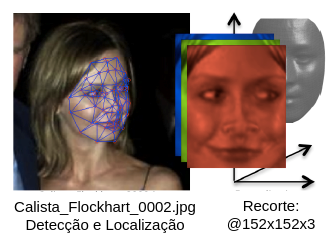
\includegraphics[scale=0.75]{figuras/detectface.png}
\caption{Detecção Facial}
\label{fig:detectface}
\end{figure}


O algoritmo Viola-Jones \citep{viola2001rapid} é amplamente usado pela comunidade para detecção facial. Esta técnica possui vantagens como alta taxa de precisão, rapidez na execução e baixa taxa de falsos positivos. Este algoritmo é utilizado por \cite{art1}, \cite{art2}, \cite{art6}, \cite{art9}, \cite{art12}, \cite{art13} e \cite{art15} para detectar a face em uma imagem e realizar o recorte com o intuito de excluir o \textit{background} da imagem, reduzindo assim a complexidade do problema e diminuindo a carga de aprendizado da rede na qual, neste caso, o classificador não necessita mais aprender a diferenciar o que é \textit{background} e face.

\subsection{Histograma de Equalização (Normalização do Brilho)}
A técnica de histograma de equalização é utilizada para normalizar o brilho da imagem \citep{jain1989fundamentals}. Obviamente há diferentes tipos de ambiente e consequentemente a iluminação pode variar bastante. Esta técnica permite que a intensidade das cores seja melhor distribuída. A atuação desta técnica equilibra o contraste da imagem nas regiões em que há ausência.

Esta técnica foi utilizada por \cite{art2}, \cite{art4} e \cite{art6}. Para todos os casos resultou no aumento da taxa de acurácia comparada a não aplicação desta técnica. Provavelmente o histograma de equalização funciona principalmente porque busca equalizar as cores da imagem retirando os ruídos de iluminação, isto é, realçando todos os pontos da imagem ocasionando maior facilidade para aprendizagem do problema devido a maximização da visibilidade nas regiões importantes que separam as classes, além disso, há a diminuição da carga de aprendizado do classificador, pois é menos necessário aprender a separar as classes nos casos de iluminação adversa.

%realçando todos os pontos da imagem ocasionando maior visibilidade das regiões importantes e o método de classificação aprende com maior facilidade a separar as classes, além disso, há a diminuição da carga de aprendizado, pois é menos necessário aprender a separar as classes nos casos de iluminação adversa.

%o primeiro por reduzir a carga de aprendizado da rede, pois nas situações em que uma imagem não possui a iluminação ideal a rede não precisa aprender essas situações adversas;

\section{Rede Neural Artificial}\label{sec:rna}
O ser humano inspirou-se nos pássaros para construir aeronaves e voar. A natureza também inspirou outras invenções da humanidade, por exemplo a dianteira de um trem-bala. Da mesma forma, as redes neurais artificiais tiveram a mesma inspiração, especificamente no cérebro, tendo como objetivo construir máquinas inteligentes \citep{geron2017hands, goodfellow2016deep}. 

Um \textit{perceptron}, que é uma simples arquitetura inspirada em um neurônio biológico, possui conexões de entrada e saída para conectar a outros neurônios. Cada conexão de entrada é associada a um peso, que recebe um sinal para o neurônio realizar uma computação baseada em uma função de ativação, gerando um sinal de saída que serve de entrada para outro neurônio \citep{geron2017hands}. 

A Figura \ref{fig:redeneural} ilustra uma rede neural \textit{perceptron} multicamadas.  A rede neural \textit{perceptron} possui uma estrutura em que consiste de uma camada de entrada, várias camadas intermediárias denominadas ocultas e uma camada de saída. Todas as camadas são compostas por neurônios \textit{perceptron}. A camada de entrada recebe os dados oriundos de uma instância, por exemplo, os \textit{pixels} de uma imagem, e encaminha os dados recebidos para a próxima camada. A camada oculta caracteriza-se por ser completamente conectada, isto é, cada neurônio conecta-se com todos da camada anterior e posterior. A camada de saída é responsável em fornecer o resultado da rede neural, por isso, nos casos de classificação, a quantidade de neurônio da camada de saída é a mesma das classes do problema. Além disso, cada neurônio da camada de saída está associada a uma classe e quando uma instância desconhecida for processada para classificação, o neurônio que terminar ativado da camada de saída representa a classificação desta instância \citep{geron2017hands, goodfellow2016deep}.

\begin{figure}
\centering
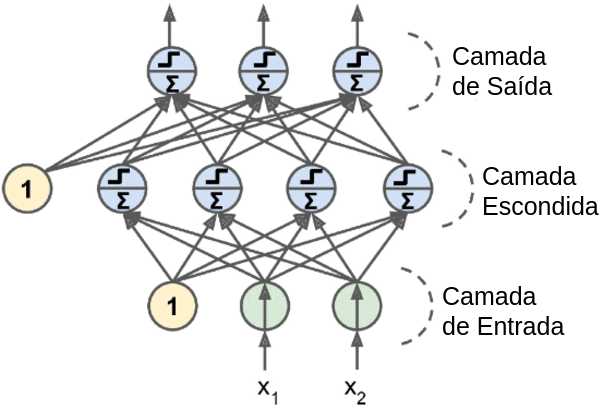
\includegraphics[scale=0.45]{figuras/redeneural.png}
\caption{Rede Neural Artificial}
\label{fig:redeneural}
\end{figure}

\section{Rede Neural de Convolução}\label{sec:rnc}
As redes neurais de convolução (RNC) surgiram dos estudos do córtex visual do cérebro e têm sido usadas em reconhecimento de imagem desde 1980 \citep{geron2017hands}. Nos últimos anos, uma série de fatores contribuíram para a evolução das RNCs, principalmente relacionados ao aumento do poder de computação (hardware), ao surgimento da web, que proporcionou o aumento da quantidade de dados para treinamento e à evolução das técnicas de treinamento de uma rede neural. Este cenário favorável permitiu que as RNCs alcançassem nível super-humano em alguns problemas complexos de visão computacional. As RNCs têm sido utilizadas em larga escala tanto pela indústria como pelos pesquisadores, sobretudo em problemas como máquinas de busca, carros autônomos, sistemas de classificação automática de vídeo e imagens, entre outras tarefas.


Os trabalhos de \cite{hubel1959single} e \cite{hubel1959receptive} realizaram uma série de experimentos em gatos em 1958, e posteriormente, em macacos \citep{hubel1968receptive}, para encontrar intuições do funcionamento do córtex visual, que é a parte cerebral responsável em processar informação visual. Estes trabalhos levaram os autores a receberem o Prêmio Nobel em Fisiologia e Medicina em 1981. Seus trabalhos mostraram que muitos neurônios do córtex visual tem um pequeno campo de recepção local, ou seja, os neurônios reagem somente a um estímulo localizado na região limitada pelo campo visual. O campo de recepção local dos diferentes neurônios podem sobrepor um ao outro e a sua combinação gera o campo visual. Os autores mostraram que alguns neurônios somente reagem às imagens com padrões de linhas horizontais enquanto outros reagem às linhas com diferentes orientações. Notou-se que alguns neurônios têm um campo grande de recepção local, consequentemente, reagindo aos padrões mais complexos. Entretanto, os neurônios estão combinando um ao outro para gerar padrões menos complexos. Estas observações são evidências de que os neurônios são baseados na saída do vizinho. 

O poderoso funcionamento do córtex visual está habilitado a detectar todos os padrões complexos em qualquer área do campo visual \citep{geron2017hands}. Todos os estudos relacionados ao córtex visual foram gradualmente inseridos nas redes neurais artificiais para gerar a rede neural de convolução. A primeira RNC  foi apresentada por \cite{lecun1998gradient}, uma arquitetura denominada LeNet-5 que foi utilizada para reconhecer dígitos escritos no papel.

\subsection{Camada de Convolução}
A camada de convolução é o mais importante bloco de uma RNC e consiste em uma operação matemática que desliza uma função sobre a outra calculando a integral entre a multiplicação de duas funções. A Figura \ref{fig:conv1} ilustra o que cada camada de convolução recebe em seu campo visual dada uma imagem como entrada na RNC. Vale ressaltar que cada neurônio da primeira camada de convolução está conectado somente a alguns campos visuais de recepção da imagem, diferentemente da abordagem tradicional que é conectada a todos os \textit{pixels}. Os neurônios da segunda camada de convolução estão conectados somente aos localizados no pequeno campo visual (retângulo) da primeira camada, novamente diferente da rede neural \textit{perceptron} em que todos os neurônios são conectados com todos da camada anterior, e assim por diante \citep{geron2017hands}. As vantagens da RNC sobre a abordagem tradicional são explicadas pela diferença entre ambas e são enfatizadas a seguir:

\begin{enumerate}[label=(\roman*)]
 \item A RNC tem característica esparsa como ilustrado na Figura \ref{fig:conv2}, por isso, a RNC possui menor quantidade de parâmetros para serem treinados do que as redes neurais tradicionais, isto é, requer menos tempo de treinamento e recursos computacionais \citep{goodfellow2016deep}; 
\item A estrutura da RNC é comum no mundo real, por exemplo no córtex visual. Essa inspiração biológica é uma das razões para RNC funcionar tão bem no reconhecimento de imagens \citep{geron2017hands}; 
\item E por fim, o compartilhamento de parâmetros resulta no aprendizado de rotações dos objetos da imagem e os neurônios aprendem em conjunto ao invés de separados \citep{goodfellow2016deep}.
\end{enumerate}


\begin{figure}
\centering
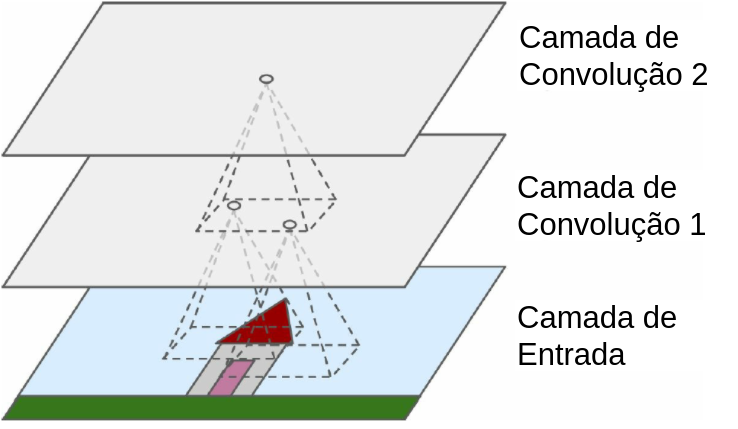
\includegraphics[scale=0.40]{figuras/conv1.png}
\caption{Camada de Convolução com campos locais de recepção}
\label{fig:conv1}
\end{figure}

\begin{figure}
\centering
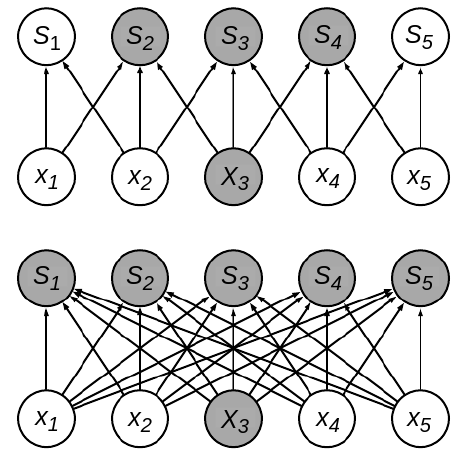
\includegraphics[scale=0.6]{figuras/conv2.png}
\caption{Conectividade esparsa. É destacada a entrada \textit{x}\textsubscript{3} e a saída em S que são afetadas por \textit{x}\textsubscript{3}. 
(Cima) Quando S recebe a convolução com um \textit{kernel} de tamanho 3, somente três saídas são afetadas por \textit{x}\textsubscript{3}. 
(Baixo) Quando S é gerado por rede neural tradicional, todos são afetados por \textit{x}\textsubscript{3}.}

%\caption{Conectividade esparsa. É destacada a entrada x\textsubscript{3} e a saída em S que são afetadas por x\textsubscript{3}}
\label{fig:conv2}
\end{figure}


\subsection{Camada de \textit{Pooling}}
Esta camada tem como foco principal realizar subamostra, isto é, diminuir o tamanho de entrada da imagem entre as camadas de convolução com objetivo de reduzir a carga computacional e o número de parâmetros, ocasionando a diminuição do risco de \textit{overfitting} e o consumo de memória \citep{geron2017hands}. Além disso, reduzir o tamanho de entrada da imagem faz a rede neural mais tolerável a variação do objeto principal, como a rotação da face. 

Geralmente uma camada de \textit{pooling} é implementada logo após uma camada de convolução, portanto recebe como entrada uma imagem processada anteriormente por uma camada de convolução com intuito de realizar subamostra da imagem e encaminhar o resultado para uma próxima camada de convolução \citep{goodfellow2016deep}.

Existem duas principais funções de \textit{pooling}. Por exemplo, o \textit{max pooling} que considera o valor máximo de um campo de recepção e está exemplificado na Figura \ref{fig:pool} por um \textit{kernel} 2x2 que elimina 75\% dos valores de entrada. Há também o \textit{pooling} pela média de um campo de recepção e seu cálculo consiste na distância entre o \textit{pixel} central e seus vizinhos \citep{goodfellow2016deep}. A camada de \textit{max pooling} é a mais comum operação de \textit{pooling} utilizada em redes neurais de convolução.


\begin{figure}
\centering
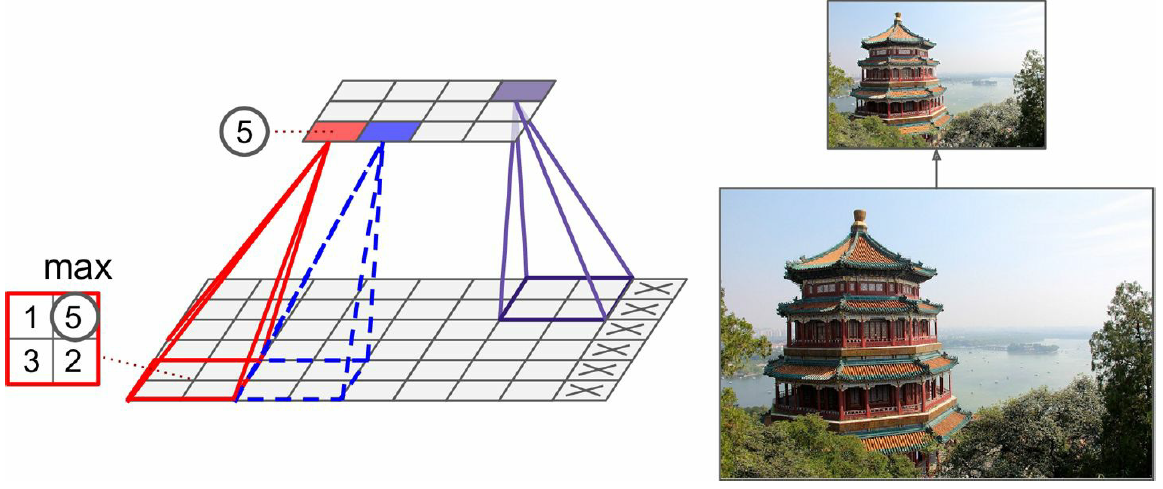
\includegraphics[scale=0.45]{figuras/pool.png}
\caption{Camada de \textit{Max Pooling}}
\label{fig:pool}
\end{figure}


\subsection{Regressão \textit{Softmax}}
Geralmente uma arquitetura de RNC é composta em sua maior parte por camadas de convolução e \textit{pooling}. Estas camadas processam a imagem com intuito de extrair os principais padrões para um classificador e determinar a classe dela. Por isso, ao final de uma arquitetura de RNC é necessário um classificador que tradicionalmente tem sido o \textit{softmax}. Este classificador é um modelo generalizado de uma regressão logística, que por sua vez é normalmente usada para estimar probabilidades de uma instância pertencer a uma classe em particular, por exemplo, qual é a probabilidade de um email ser spam? \citep{geron2017hands}. Se a estimativa de probabilidade for maior que 50\%, então o modelo prevê que a instância pertence a classe positiva, caso contrário, pertence à classe negativa. Portanto, isto faz do regressor logístico um classificador binário. Um \textit{softmax} é capaz de estimar probabilidades para múltiplas classes e não há a necessidade de treinar e combinar múltiplos classificadores binários para tal tarefa. Um \textit{softmax} está habilitado a estimar probabilidades para uma imagem processada em uma RNC e, para todos os efeitos, a imagem é uma expressão facial que pertence às emoções básicas: neutralidade, felicidade, surpresa, medo, raiva, tristeza ou desgosto.

\section{Arquiteturas de Redes Neurais de Convolução}\label{sec:arc}
\subsection{AlexNet}

A arquitetura AlexNet foi desenvolvida por Alex Krizhevsky (por isso, o nome da mesma), Ilya Sutskever e Geoffrey Hinton. Destacando-se por ser grande e muito profunda, a AlexNet foi a primeira RNC a empilhar camadas de convolução diretamente em cima da outra, ao invés da tradicional conexão entre uma camada de convolução e a camada de \textit{pooling}. Esta arquitetura pode ser consultada na Tabela \ref{alexnet}.

A AlexNet usa uma normalização bastante eficiente entre as camadas C1 e C3 denominada \textit{local response normalization}. Essa forma de normalização causa um efeito que contribui para inibição dos neurônios em ativar mais fortemente no mesmo local, ocasionando que outros mapas de características se tornem também especialistas em determinada região da imagem. Este comportamento também é observado nos neurônios biológicos \citep{geron2017hands}. 

O seu grande sucesso foi devido ao desafio de 2012 do ImageNet ILSVRC, que tem sido o principal concurso de classificação de imagens organizado pela comunidade científica, em que venceu por uma margem bastante grande: alcançou 17\% no top-5 da taxa de erro, enquanto o segundo melhor alcançou somente 26\%!

\begin{table}[]
\caption{Arquitetura AlexNet}
\centering
\begin{tabular}{|c|c|c|c|c|c|}
\hline
\textbf{Camada} & \textbf{Tipo}           & \textbf{Mapas} & \textbf{Tamanho} & \textbf{Kernel} & \textbf{Ativação} \\ \hline
Saída           & Completamente Conectada & -              & 1000             & -               & Softmax           \\ \hline
F9              & Completamente Conectada & -              & 4096             & -               & ReLU              \\ \hline
F8              & Completamente Conectada & -              & 4096             & -               & ReLU              \\ \hline
C7              & Convolução              & 256            & 13 x 13          & 3 x 3           & ReLU              \\ \hline
C6              & Convolução              & 384            & 13 x 13          & 3 x 3           & ReLU              \\ \hline
C5              & Convolução              & 384            & 13 x 13          & 3 x 3           & ReLU              \\ \hline
S4              & \textit{Max Pooling}    & 256            & 13 x 13          & 3 x 3           & -                 \\ \hline
C3              & Convolução              & 256            & 27 x 27          & 5 x 5           & ReLU              \\ \hline
S2              & \textit{Max Pooling}    & 96             & 27 x 27          & 3 x 3           & -                 \\ \hline
C1              & Convolução              & 96             & 55 x 55          & 11 x 11         & ReLU              \\ \hline
Entrada         & Entrada                 & 3 (RGB)        & 224 x 224        & -               & -                 \\ \hline
\end{tabular}
%\caption{AlexNet arquitetura}
%\label{my-label}
\label{alexnet}
\end{table}


\subsection{GoogLeNet}

A arquitetura GoogLeNet \citep{szegedy2015going} foi desenvolvida por Christian Szegedy do \textit{Google Research}, e venceu o desafio do ILSVRC 2014 por alcançar a taxa de erro no top-5 abaixo de 7\%. Este grande desempenho foi devido em grande parte pelo fato de que a rede foi muito mais profunda do que as anteriores. O aumento de profundidade está diretamente relacionado à criação de sub-redes chamadas de \textit{inception} e está ilustrada na Figura \ref{fig:inception}. Essas sub-redes permitiram que a GoogLeNet utilizasse os parâmetros de forma mais eficiente comparada às arquiteturas anteriores e a dimensão desta eficiência pode ser elucidada pela diferença de parâmetros entre a GoogLeNet e a AlexNet, em que a primeira possui 10 vezes menos parâmetros do que a segunda \citep{geron2017hands}. 

Um módulo \textit{inception}, que está ilustrado na Figura \ref{fig:inception}, possui uma notação ''3 x 3 + 2 (S)''. Isto significa que a camada usa um \textit{kernel} 3 x 3, \textit{stride} 2 e \textit{SAME padding}. O sinal de entrada é primeiramente copiado e alimenta as camadas do módulo \textit{inception} que estão divididas em dois conjuntos. O primeiro conjunto recebe o sinal para processar e encaminhar para o segundo. Vale ressaltar que todas as camadas de convolução utilizam a ReLU como função de ativação. É interessante observar que o segundo conjunto usa diferentes tamanhos de \textit{kernel} (1 x 1, 3 x 3 e 5 x 5), permitindo que a rede possa capturar diferentes padrões de escala \citep{geron2017hands}. No fim do módulo, há uma camada de concatenação, isto é, combina todas as saídas do segundo conjunto de camadas de convolução e encaminha um único sinal que é o resultado do módulo para uma próxima camada da rede. A rede GoogLeNet é composta por módulos \textit{inception}, camadas de convolução, \textit{max pooling}, camadas de \textit{local normalization response}, camadas completamente conectadas e \textit{softmax}.


\begin{figure}
\centering
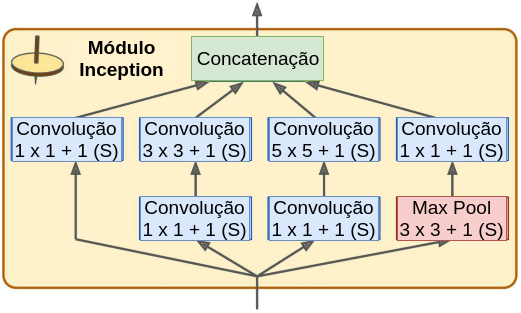
\includegraphics[scale=0.6]{figuras/inception.png}
\caption{Módulo \textit{inception}}
\label{fig:inception}
\end{figure}


\subsection{VGGNet}
Proposta por \cite{simonyan2014very}, a VGGNet foi a vice-campeã do desafio ILSVRC 2014, tendo alcançado 6.8\% na taxa de erro top-5. A sua principal contribuição foi uma avaliação exaustiva de seis RNCs, que consistiu no aumento de profundidade enfatizando a utilização de filtros de convolução com tamanho muito pequeno (3 x 3), promovendo o aumento da profundidade da rede que passou de 16 para 19 camadas. Esta abordagem mostrou um aumento de eficiência significativo comparado às técnicas anteriores. 

A VGGNet é composta principalmente por camadas de convolução, \textit{max pooling}, completamente conectadas e \textit{softmax}, e está ilustrada na Tabela \ref{tab:vgg}. O fato de usar filtros de convolução com tamanho pequeno ocasionou no não aumento do número de parâmetros a serem ajustados a medida que a rede cresce, promovendo assim a eficiência.

%\begin{figure}
%\centering
%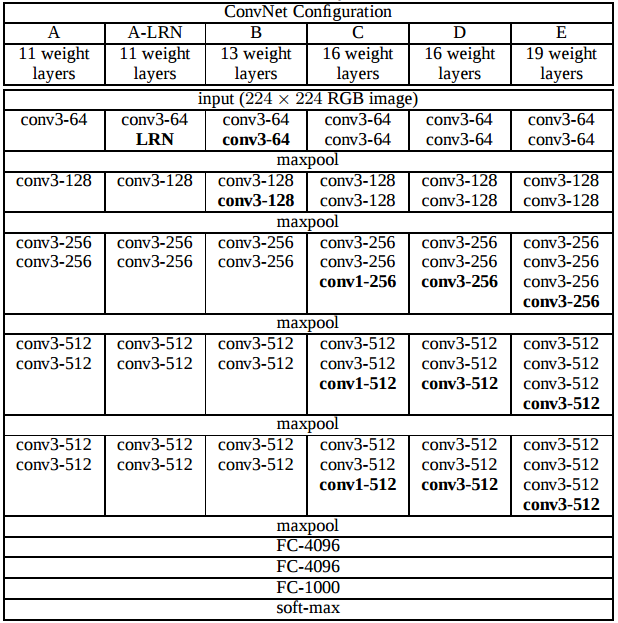
\includegraphics[scale=0.6]{figuras/vgg.png}
%\caption{VGGNet}
%\label{fig:vgg}
%\end{figure}


\begin{table}[]
\centering
\caption{Arquiteturas VGGNet}
\label{tab:vgg}
\begin{tabular}{|c|c|c|c|c|c|}
\hline
\multicolumn{6}{|c|}{\textbf{VGGNet configuração}}                                                                                                                                                                                                                                                                                                                                                                                               \\ \hline
A                                                             & A-LRN                                                         & B                                                             & C                                                                         & D                                                                         & E                                                                                     \\ \hline
11 camadas                                                    & 11 camadas                                                    & 13 camadas                                                    & 16 camadas                                                                & 16 camadas                                                                & 19 camadas                                                                            \\ \hline
\multicolumn{6}{|c|}{camada de entrada (224 x 224 imagem RGB)}                                                                                                                                                                                                                                                                                                                                                                                \\ \hline
conv3-64                                                      & \begin{tabular}[c]{@{}c@{}}conv3-64\\ \textbf{LRN}\end{tabular}        & \begin{tabular}[c]{@{}c@{}}conv3-64\\ \textbf{conv3-64}\end{tabular}   & \begin{tabular}[c]{@{}c@{}}conv3-64\\ conv3-64\end{tabular}               & \begin{tabular}[c]{@{}c@{}}conv3-64\\ conv3-64\end{tabular}               & \begin{tabular}[c]{@{}c@{}}conv3-64\\ conv3-64\end{tabular}                           \\ \hline
\multicolumn{6}{|c|}{maxpool}                                                                                                                                                                                                                                                                                                                                                                                                                 \\ \hline
conv3-128                                                     & conv3-128                                                     & \begin{tabular}[c]{@{}c@{}}conv3-128\\ \textbf{conv3-128}\end{tabular} & \begin{tabular}[c]{@{}c@{}}conv3-128\\ conv3-128\end{tabular}             & \begin{tabular}[c]{@{}c@{}}conv3-128\\ conv3-128\end{tabular}             & \begin{tabular}[c]{@{}c@{}}conv3-128\\ conv3-128\end{tabular}                         \\ \hline
\multicolumn{6}{|c|}{maxpool}                                                                                                                                                                                                                                                                                                                                                                                                                 \\ \hline
\begin{tabular}[c]{@{}c@{}}conv3-256\\ conv3-256\end{tabular} & \begin{tabular}[c]{@{}c@{}}conv3-256\\ conv3-256\end{tabular} & \begin{tabular}[c]{@{}c@{}}conv3-256\\ conv3-256\end{tabular} & \begin{tabular}[c]{@{}c@{}}conv3-256\\ conv3-256\\ \textbf{conv1-256}\end{tabular} & \begin{tabular}[c]{@{}c@{}}conv3-256\\ conv3-256\\ \textbf{conv3-256}\end{tabular} & \begin{tabular}[c]{@{}c@{}}conv3-256\\ conv3-256\\ conv3-256\\ \textbf{conv3-256}\end{tabular} \\ \hline
\multicolumn{6}{|c|}{maxpool}                                                                                                                                                                                                                                                                                                                                                                                                                 \\ \hline
\begin{tabular}[c]{@{}c@{}}conv3-512\\ conv3-512\end{tabular} & \begin{tabular}[c]{@{}c@{}}conv3-512\\ conv3-512\end{tabular} & \begin{tabular}[c]{@{}c@{}}conv3-512\\ conv3-512\end{tabular} & \begin{tabular}[c]{@{}c@{}}conv3-512\\ conv3-512\\ \textbf{conv1-512}\end{tabular} & \begin{tabular}[c]{@{}c@{}}conv3-512\\ conv3-512\\ \textbf{conv3-512}\end{tabular} & \begin{tabular}[c]{@{}c@{}}conv3-512\\ conv3-512\\ conv3-512\\ \textbf{conv3-512}\end{tabular} \\ \hline
\multicolumn{6}{|c|}{maxpool}                                                                                                                                                                                                                                                                                                                                                                                                                 \\ \hline
\begin{tabular}[c]{@{}c@{}}conv3-512\\ conv3-512\end{tabular} & \begin{tabular}[c]{@{}c@{}}conv3-512\\ conv3-512\end{tabular} & \begin{tabular}[c]{@{}c@{}}conv3-512\\ conv3-512\end{tabular} & \begin{tabular}[c]{@{}c@{}}conv3-512\\ conv3-512\\ \textbf{conv1-512}\end{tabular} & \begin{tabular}[c]{@{}c@{}}conv3-512\\ conv3-512\\ \textbf{conv3-512}\end{tabular} & \begin{tabular}[c]{@{}c@{}}conv3-512\\ conv3-512\\ conv3-512\\ \textbf{conv3-512}\end{tabular} \\ \hline
\multicolumn{6}{|c|}{maxpool}                                                                                                                                                                                                                                                                                                                                                                                                                 \\ \hline
\multicolumn{6}{|c|}{camada completamente conectada - 4096}                                                                                                                                                                                                                                                                                                                                                                                   \\ \hline
\multicolumn{6}{|c|}{camada completamente conectada - 4096}                                                                                                                                                                                                                                                                                                                                                                                   \\ \hline
\multicolumn{6}{|c|}{camada completamente conectada - 1000}                                                                                                                                                                                                                                                                                                                                                                                   \\ \hline
\multicolumn{6}{|c|}{softmax}                                                                                                                                                                                                                                                                                                                                                                                                                 \\ \hline
\end{tabular}
\end{table}

\subsection{Residual Network}
A Residual Network (ou ResNet) foi desenvolvida por \cite{he2016deep} e foi a técnica vencedora do desafio ILSVRC 2015. A ResNet foi avaliada na base de teste do ImageNet que tinha 1000 classes e alcançou 3.6\% em taxa de erro no top-5. Este tipo de avaliação consiste na verificação das 5 classes com maiores probabilidades após uma classificação, e caso esta imagem de fato pertencer ao grupo das 5 classes é caracterizado uma classificação correta. A ResNet proposta para o concurso tinha 152 camadas caracterizando uma rede muito profunda. 

O segredo desta técnica consiste na composição dos blocos residuais. A novidade desta arquiteutra é possibilitar que um bloco residual faça o mapeamento de outros blocos distantes através de conexões de salto, isto é, os sinais emitidos pelos neurônios tanto na direção para frente como para trás podem ser propagados diretamente de um bloco para qualquer outro bloco como ilustrado na Figura \ref{fig:bloco-residual}. Este tipo de conexão trouxe impactos positivos na aprendizagem, principalmente atuando na função objetiva, pois quando a mesma está próxima de convergir é aumentado consideravelmente a velocidade do treino comparada as redes tradicionais sem as conexões de salto.   

\begin{figure}
\centering
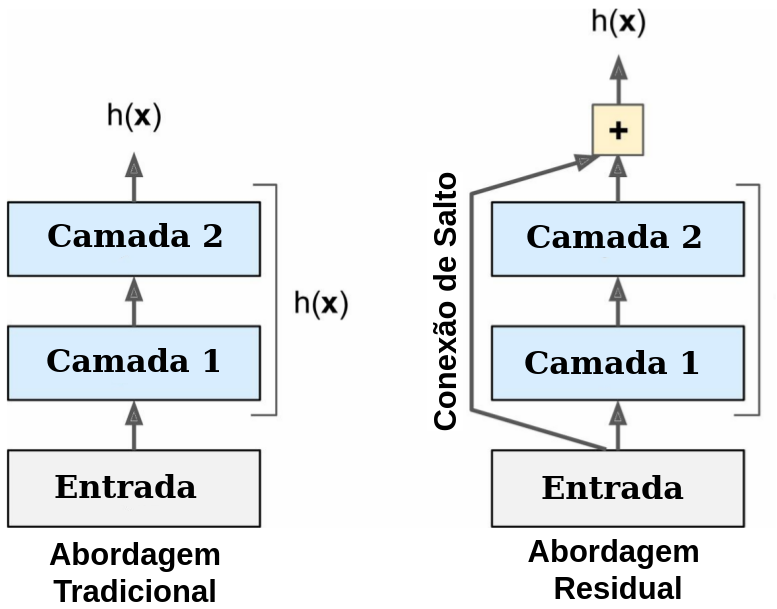
\includegraphics[scale=0.36]{figuras/resnet-block-residual.png}
\caption{Bloco residual}
\label{fig:bloco-residual}
\end{figure}


\subsection{\textit{Ensemble}}
Suponha uma questão complexa perguntada aleatoriamente para milhões de pessoas, então, todas as respostas são agregadas para obter o resultado. Em muitos casos, a resposta agregada é melhor do que a de um especialista. Isto é conhecido como sabedoria popular. Similarmente, se agregar as classificações de uma determinada instância oriunda de um grupo de RNCs e, frequentemente, tem mais acertos do que a classificação de uma única RNC. Um grupo de RNCs ou outros tipos de classificadores e regressores são chamados de \textit{ensemble} \citep{geron2017hands}. Geralmente, quem trabalha com \textit{ensemble} no problema de reconhecimento de emoção tem calculada a média das probabilidades estimadas pelas diversas RNCs para decidir qual a classificação final da expressão facial.

\section{Métricas de Avaliação de Desempenho para Classificadores}\label{sec:metavalclass}
As principais métricas utilizadas para avaliação de desempenho de classificadores são: acurácia, precisão, revocação e f1-score. Por meio dessas métricas é possível comparar os classificadores determinando os pontos fortes e fracos, invertigar quais são as classes que o modelo tem maiores desempenho, verificar a existência de \textit{overfitting} em uma classe específica, e também, se houve aprendizado em classes com menores amostras. É relevante tais verificações, pois quando a base de treino é desbalanceada pode gerar um modelo que consiste de chutar as classes com maiores amostras a fim de maximizar as taxas de acertos, no entanto, claramente caracterizando um modelo com \textit{overfitting}.

A acurácia é a proporção dos casos corretamente classificados e é calculada a partir da Equação \ref{fun:acurracy}, em que TP é a taxa de verdadeiros positivos, TN é a taxa de verdadeiros negativos, FP é a taxa de falsos positivos e FN é a taxa de falsos negativos. A precisão nos diz a fração de instâncias que são verdadeiras positivas de um grupo que o classificador preveu ser positvo e a fórmula pode ser consultada em \ref{fun:precision}. A revocação mede a fração de instâncias positivas que o classificador esqueceu de classificar corretamente (Equação \ref{fun:recall}). 

Classificadores com uma taxa de revocação alta não tem muitas instâncias positivas classificadas incorretamente. Vale destacar que facilmente é possível construir um classificador que alcança altas taxas de precisão ou revocação mas não ambos. Caso o classificador prevê todas as instâncias da classe positiva, o modelo teria uma taxa perfeita de revocação, entretanto uma baixa precisão. Por isso, criar um classificador que maximiza tanto precisão como revocação é um desafio.

É frequentemente conveniente combinar precisão e revocação em uma única métrica chamada de f1-score, principalmente quando é necessário comparar de uma simples maneira dois classificadores. A f1-score é a média harmônica de precisão e revocação (Equação \ref{fun:f1-score}). Enquanto a média tradicional trata todos os valores igualmente, isto é, sem pesos, a média harmônica favorece os valores mais baixos. Portanto, caso tenha alta revocação e baixa precisão, o resultado de f1-score será mais próximo de precisão, pois esta métrica adiciona pesos nos valores mais baixos, que neste caso é o valor de precisão.  

\begin{equation}
\label{fun:acurracy}
acurácia = \frac{TP + TN}{TP + TN + FP + FN} 
\end{equation}


\begin{equation}
\label{fun:precision}
precisão = \frac{TP}{TP + FP} 
\end{equation}

\begin{equation}
\label{fun:recall}
revocação = \frac{TP}{TP + FN} 
\end{equation}

\begin{equation}
\label{fun:f1-score}
f1-score = \frac{2}{\frac{1}{precisaão} + \frac{1}{revocação}} = 2 * \frac{precisão * revocação}{precisão + revocação}
\end{equation}



%\subsection{Precisão}
%\subsection{Revocação}
%\subsection{F1-score}

\section{Resumo}\label{sec:considf}
Neste capítulo foram apresentados os principais conceitos utilizados por esta proposta. Foi visto que uma RNC, que é uma técnica de aprendizagem de máquina, foi projetada para a classificação de imagem, justificando a sua escolha para a classificação de emoções em expressão facial. Esta técnica é muito poderosa e tem sido inspirada no cérebro dos mamíferos. A expressão facial tem se destacado como uma forma eficaz de coleta de dados para o reconhecimento de emoção, principalmente, por ser ubíqua, não intrusiva e pela popularidade de dispositivos que contém câmeras fotográficas. Entretanto, somente as emoções básicas são possíveis de reconhecer por meio da expressão facial. Isso significa que reconhecer tédio, frustração e confusão se torna bastante difícil por esse meio. Além disso, técnicas de pré-processamento, tais como histograma de equalização e detecção com recorte da face são úteis durante o processo de classificação de imagens, justamente por diminuir a carga de aprendizado da rede. Por fim, foram conceituadas algumas das principais arquiteturas de RNCs em que cada uma possui sua característica em particular que precisam ser experimentadas em diferentes cenários.  


\chapter{Trabalhos Correlatos}\label{sec:relacionados}
Os trabalhos relacionados são discutidos neste capítulo e está organizado da seguinte forma.  Na Seção \ref{sec:edc} analisa as principais extrações de características encontradas na literatura para o processamento da expressão facial. Na Seção \ref{sec:arct} avalia os trabalhos correlatos categorizados pelas arquiteturas de RNC. Na Seção \ref{sec:apl} é comentado as aplicações para o reconhecimento de emoção por expressão facial e enquanto a Seção \ref{sec:cons} faz um resumo a respeito deste capítulo.


\section{Preparação dos dados}\label{sec:dataprepared}
Os problemas de classificação em geral, seja de imagem, vídeo, áudio ou qualquer tipo, tradicionalmente sofrem pela ausência de dados. Algoritmos de aprendizagem de máquina requerem quantidade de dados expressivos para apresentar soluções com desempenho satisfatório, especificamente as redes neurais profundas. Raramente há dados disponíveis e que sejam suficientes para treinar e validar uma rede neural de convolução, vale ressaltar que cada problema tem sua particularidade, isto é, quanto maior a complexidade mais dados são necessários. 

Contudo, a comunidade de reconhecimento de emoção para amenizar esse problema utiliza a técnica de aumento de dados e multiplicação de imagens. Essa técnica consiste na geração de cópias de uma imagem original, que contém uma expressão facial, para gerar imagens duplicadas. Entretanto, tais imagens duplicadas são diferentes da imagem original, justamente por possuir alterações na posição da face com leves rotações da mesma, variação da intensidade das cores e redimensionamento com aplicação de \textit{zoom}. As imagens aumentadas são usadas durante o treinamento contribuindo para a rede neural aprender a reconhecer emoção em diferentes rotações, intensidade de iluminação e escala. 

Os trabalhos de \cite{art4, art6, art7, art8, art11} e \cite{art15} utilizaram a técnica de aumento de dados. A técnica foi configurada para aumentar entre 5 a 10 vezes cada imagem original. Sendo assim, a base de dados original foi ampliada em até 10 vezes, gerando um ganho considerável dos dados. Tais trabalhos alcançaram boas taxas de reconhecimento em que o \emph{fine tuning} dos modelos possuem generalização adequada e não apresentando \emph{overfitting} e \emph{underfitting}. O resultado expressivo foi viabilizado pela técnica de aumento de dados justamente pela rede ser treinada e validada com maiores quantidades de dados. 
%tais imagens duplicadas possuem alterações na posição da face aplicando leves rotações da imagem original gerando novas imagens válidas tanto para treinamento como para validação.      

%\section{Metodologia de Treinamento e Validação}\label{sec:trainingValidationMethodology}


\section{Extração de Característica}\label{sec:edc}
Uma etapa essencial durante o processo de classificação de imagem é a extração de característica. A extração de característica é sucintamente enfatizada na Seção \ref{sec:pci} e tem como finalidade destacar ou retirar as formas mais relevantes da imagem que são cruciais para a separação das classes. A seguir, os principais tipos de extração de características empregados para o reconhecimento de emoção por expressão facial são analisados.

\subsection{Extração Geométrica}
A extração de características geométrica consiste na obtenção de pontos faciais ilustradas pela Figura \ref{fig:geometrica}. As características geométricas tem como finalidade capturar as deformações na face causadas pela ativação dos músculos a partir dos pontos faciais \citep{art11}. Esses pontos faciais podem ser mapeados pelos seguintes métodos: \cite{yu2016face} e \cite{yu2014consensus}.
A extração geométrica é uma abordagem que realiza medições entre diversas partes da face tais como:

\begin{enumerate}[label=(\roman*)]
\item Altura da sobrancelha esquerda/direita (distância vertical entre o ponto mais superior da sobrancelha e centro do olho);  
\item Altura da pálpebra esquerda/direita (distância vertical entre o ponto mais superior do olho e parte inferior do olho);  
\item Altura do nariz (distância vertical entre o ponto mais inferior do olho para o nariz e centro de ambos os olhos);  
\item Largura do nariz (distância horizontal entre os pontos do nariz mais à esquerda e à direita);  
\item Altura do lábio superior (distância vertical entre o ponto mais superior e o centro da boca); 
\item Altura do lábio inferior (distância vertical entre o ponto mais inferior e o centro da boca); 
\item A distância do ponto da boca mais a esquerda para o centro da boca; 
\item E por fim, a distância do ponto da boca mais a direita para o centro da boca.
\end{enumerate}

A extração geométrica é amplamente empregada nas abordagens tradicionais de aprendizado de máquina, isto é, abordagens que não utilizam as redes neurais de convolução. Todavia, o trabalho de \cite{art11} realiza a extração geométrica concatenando com a RNC e obteve um pequeno ganho na taxa de precisão de 1\%. Um diagrama da sua abordagem é ilustrada na Figura \ref{fig:yun-customizing}. No entanto, a combinação entre a extração geométrica e RNC, obviamente, aumenta o custo computacional devido a outros algoritmos serem executados como o mapeamento dos pontos faciais e as suas distâncias. Caso o foco do reconhecedor de emoções for aplicações em cenários reais, provavelmente, não é viável a concatenação devido o aumento na taxa de reconhecimento ser baixo, portanto não compensada pelo aumento do custo computacional, pois tais cenários requerem classificação instantânea e em tempo real.

\begin{figure}
\centering
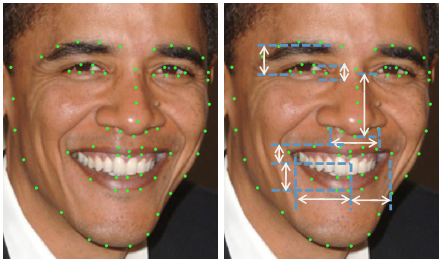
\includegraphics[scale=0.45]{figuras/tipogeo.png}
\caption{Extração dos pontos faciais para características geométrica}
\label{fig:geometrica}
\end{figure}

\begin{figure}
\centering
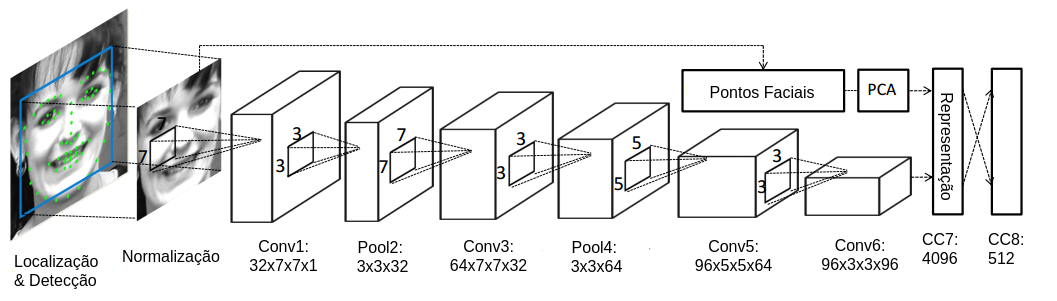
\includegraphics[scale=0.48]{figuras/yun-customizing.png}
\caption{Concatenação dos pontos faciais com uma rede neural de convolução}
\label{fig:yun-customizing}
\end{figure}



\subsection{Extração Aparente}
A extração de característica aparente considera as sub-regiões faciais, principalmente próximas da boca e dos olhos, como características essenciais para a classificação, diferentemente, das características geométricas que foca na captura das deformações dos pontos faciais e possui como desvantagem não considerar as mudanças aparentes causadas por essas deformações capturadas \citep{art11}. A  extração aparente foi amplamente estudada por \cite{ekman1994}, encontrando 96 unidades de ações (ou sub-regiões) na face correspondentes a movimentação de diversos músculos relacionada a uma determinada emoção. A RNC está habilitada naturalmente a realizar a extração de característica aparente, sendo assim, o processo de aprendizado está associado a descoberta de quais as sub-regiões da face mais relevantes para determinar qual a emoção está emitida em uma face. A Figura \ref{fig:aparente} ilustra as sub-regiões de uma face que são interessantes para a classificação depois de um processo de aprendizado.


\begin{figure}
\centering
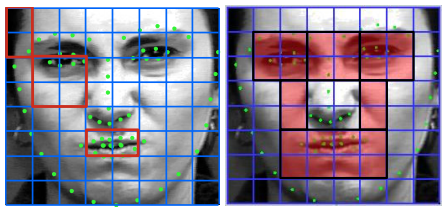
\includegraphics[scale=0.47]{figuras/tipoapa.png}
\caption{Extração das sub-regiões faciais para características aparente}
\label{fig:aparente}
\end{figure}

\section{Arquiteturas}\label{sec:arct}
\subsection{AlexNet}
A arquitetura AlexNet foi a RNC mais encontrada na literatura para reconhecimento de emoção, principalmente por ter sido a pioneira da família de métodos conhecido como aprendizado profundo que fez grande sucesso, inclusive esta rede venceu o desafio ILSVRC-2012. O trabalho de \cite{art4} utiliza AlexNet para reconhecer emoções, a sua abordagem é destacada por combinar a AlexNet com uma rede profunda \textit{autoencoder} para alinhamento de face, esta foi uma grande contribuição do autor que apresentou uma solução funcional para o problema de rotação ou desalinhamento da face. O trabalho de \cite{art2} propõe uma abordagem que consiste no emprego da técnica de equalização de histograma durante a fase de pré-processamento com intuito de resolver o problema da iluminação, desta forma, foi mostrado que a aplicação da técnica melhorava o aprendizado da rede. Nos trabalhos que utilizaram a AlexNet é notável que para alcançar maiores taxas de reconhecimento foi necessário o emprego de técnicas de pré-processamento. 

\subsection{VGG}
\cite{art8} utilizou uma VGG de 13 camadas, isto é, uma arquitetura bastante profunda inclusive com camadas de \textit{dropout} para alcançar maior generalização. Utilizou a técnica de aumento de dados, isto é, gerou novas imagens multiplicando por 10 a imagem original, as imagens geradas tinham variações da pose da face, pequenas rotações que contribuem para o aprendizado da rede. No trabalho de \cite{art13}, abordou a transferência de aprendizado para melhorar a performance de classificação, a VGG utilizada anteriormente tinha sido pré-treinada com a base do \textit{ImageNet} (do tradicional desafio ILSVRC), que é uma base que contém dezenas de objetos, e então, foi realizado um segundo auto-ajuste (treinamento) para a classificação das expressões faciais.

\subsection{GoogLeNet}
\cite{art10} realizou um trabalho comparando a arquitetura \textit{GoogLeNet} com a \textit{AlexNet}. A primeira alcançou melhores resultados, principalmente por possuir camadas \textit{inceptions} que são arquiteturas mais otimizadas para a classificação de imagens. Neste trabalho, também foi testado o classificador \textit{kNN} na última camada, que alcançou melhor resultado que o tradicional \textit{softmax}. Entretanto, vale ressaltar que, o \textit{kNN} é uma técnica baseada em instâncias, isto é, não aprende e consequentemente não gera um modelo. Em outras palavras, caso haja 100\textit{k} imagens na base de treino, o \textit{kNN} para classificar qualquer instância aleatória da base de teste ou validação necessita realizar um conjunto de cálculos de distâncias entre as 100\textit{k} imagens da base de treino para encontrar a classificação da instância, implicando em uma grande desvantagem pois este processo é repetido para cada instância que se deseja classificar.


\subsection{Ensemble}
Os trabalhos que utilizaram \textit{Ensemble} combinaram CNN com outas técnicas ou com outras CNN. No trabalho realizado por \cite{art3} foram combinadas até 100 CNNs, no qual obteve melhor resultado que uma CNN sozinha. Entretanto, foi verificado que poucas CNNs, isto é, menos de 10, já alcançam o mesmo resultado que 100 CNNs juntas, ou seja, o aprendizado fica estável se continuar aumentando a quantidade de CNN a partir de um limiar. Isto implica que menos de 10 CNNs combinadas, é o suficiente para aprender o problema de reconhecimento de emoção por expressão facial. \cite{art5} implementou um \textit{ensemble} de 3 CNNs com um único classificador \textit{softmax} que recebia a extração de características das 3 CNNs. No trabalho de \cite{art6} foi treinada 20 redes diferentes com 5 entradas diferentes, também, foi testado a utilização do classificador Support Vector Machine (SVM) ao invés do tradicional \textit{softmax} na última camada, e o Support Vector Machine alcançou resultados melhores.

%\begin{table}[]\footnotesize
%\centering
%\begin{tabular}{|c|L|}
%\hline
%\textbf{Arquitetura} & \textbf{Trabalhos que utilizaram a arquitetura}                                                                                    \\ \hline
%AlexNet              & \cite{art1}, \cite{art2}, \cite{art4}, \cite{art7}, \cite{art9}, \cite{art11}, \cite{art13}, \cite{art14}, \cite{art15} \\ \hline
%GoogLeNet            & \cite{art10}                                                                                            \\ \hline
%VGG                  & \cite{art8}, \cite{art13}                                                                                 \\ \hline
%Ensemble             & \cite{art3}, \cite{art5}, \cite{art6}                                                                       \\ \hline
%\end{tabular}

%\caption{Arquiteturas}
%\label{arquitetura}

%\end{table}

\begin{table}[]
\centering
\caption{Principais arquiteturas de Redes Neurais de Convolução para reconhecimento de expressões faciais. (*) Significa que a rede foi treinada (\emph{fine-tuning}) por duas vezes.}
\label{my-label}
\begin{tabular}{|c|c|c|c|c|}
\hline
\textbf{Arquitetura} & \textbf{Trabalho} & \textbf{Base de Treino} & \textbf{Base de Validação} & \textbf{Acurácia} \\ \hline
\multirow{15}{*}{AlexNet} & \multirow{3}{*}{\cite{art1}} & CK+ & CK+ & 99.1\% \\ \cline{3-5} 
 &  & CK+ & JAFFE & 83.11\% \\ \cline{3-5} 
 &  & JAFFE & JAFFE & 87.7\% \\ \cline{2-5} 
 & \multirow{2}{*}{\cite{art2}} & JAFFE & JAFFE & 76.7\% \\ \cline{3-5} 
 &  & CK+ & CK+ & 80.3\% \\ \cline{2-5} 
 & \cite{art4} & FER & FER & 73.73\% \\ \cline{2-5} 
 & \multirow{2}{*}{\cite{art7}} & FER & FER & 76.9\% \\ \cline{3-5} 
 &  & CK+ & CK+ & 97.3\% \\ \cline{2-5} 
 & \cite{art9} & CK+ & CK+ & 96.04\% \\ \cline{2-5} 
 & \multirow{2}{*}{\cite{art11}} & CK+ & CK+ & 98.7\% \\ \cline{3-5} 
 &  & MMI & MMI & 98.6\% \\ \cline{2-5} 
 & \cite{art13}* & FER/EmotiW & FER/EmotiW & 55.6\% \\ \cline{2-5} 
 & \cite{art14} & CK+/FER & CK+/FER & 86.54\% \\ \cline{2-5} 
 & \multirow{2}{*}{\cite{art15}} & CIFE & CIFE & 81.5\% \\ \cline{3-5} 
 &  & CK+ & CK+ & 83\% \\ \hline
\multirow{2}{*}{VGG} & \cite{art8} & FER+ & FER+ & 84.9\% \\ \cline{2-5} 
 & \cite{art13}* & FER/EmotiW & FER/EmotiW & 52.1\% \\ \hline
GoogLeNet & \cite{art10} & FER/SFEW2.0 & FER/SFEW2.0 & 71.3\% \\ \hline
\multirow{10}{*}{Ensemble} & \multirow{4}{*}{\cite{art3}} & FER & FER-Private & 69.96\% \\ \cline{3-5} 
 &  & FER & CK+ & 76.05\% \\ \cline{3-5} 
 &  & FER & JAFFE & 50.70\% \\ \cline{3-5} 
 &  & FER & EmotiW & 34.09\% \\ \cline{2-5} 
 & \cite{art5} & FER & FER & 65.03\% \\ \cline{2-5} 
 & \multirow{5}{*}{\cite{art6}} & \multirow{5}{*}{FER/SFEW} & FER-Test & 66.67\% \\ \cline{4-5} 
 &  &  & SFEW & 64.84\% \\ \cline{4-5} 
 &  &  & CK+ & 65.54\% \\ \cline{4-5} 
 &  &  & KDEF & 50.66\% \\ \cline{4-5} 
 &  &  & JAFFE & 49.17\% \\ \hline
\end{tabular}
\end{table}



\section{Aplicações}\label{sec:apl}
Há diversas aplicações para o reconhecimento de emoção no mundo real, foi percebido que os pesquisadores de reconhecimento de emoção por expressão facial utilizando RNC, ultimamente concentraram seus esforços mais no desenvolvimento de reconhecedores de emoção do que a aplicação em cenários reais, mesmo assim, está aberto para trabalhos futuros inúmeras aplicações desses reconhecedores em diversas áreas, tendo destaque principalmente para: 

\begin{itemize}
\item Interação humano computador \citep{art1, art3, art5, art8}, onde pode ser possível projetar interfaces que se adaptam ao estado emocional do usuário;
\item Psiquiatria e cuidados médicos \citep{art1, art3, art12}, no qual o reconhecedor de emoção deve monitorar constantemente o paciente ou usuário fornecendo dados emocionais que podem contribuir para diagnósticos;
\item Deficiente visual \citep{art15}, pois pessoas com alto grau de deficiência visual, tem dificuldades na interação entre pessoas para identificar qual a emoção que as pessoas em volta estão emitindo;
\item Interação humano robô \citep{art6, art14}, fazendo com que robôs estejam habilitados a interagir com humanos podendo adaptar-se a emoção dos humanos em volta, ou até mesmo emitir emoção se aproximando de um humanoide;
\item Personagens virtuais e animação \citep{art9, art11}, habilitando avatares a copiar expressão humana que podem ser útil para gravações de filmes de animação, também pode ser usado em aplicações de animação como o popular aplicativo para \textit{smartphone} o \textit{Snapchat}, que identifica a expressão facial do usuário e retorna alguma animação sobrepondo a expressão anteriormente detectada do usuário.
\end{itemize}

\section{Resumo}\label{sec:cons}
Neste capítulo foram apresentado os trabalhos relacionados, verificamos que o tema está em crescente investigação pela comunidade, visto que arquiteturas poderosas de RNC surgiram recentemente. Apesar de uma RNC ter embutido o pré-processamento em sua própria arquitetura, para o problema tratado por este trabalho, verificamos que pré-processamento adicionais (não originais da RNC) melhoraram consideravelmente a taxa de acurácia. É importante frisar que as principais arquiteturas empregadas tem sido as vencedoras ou com pouca variação do tradicional problema de aprendizado profundo: o desafio ILSVRC. Estas arquiteturas tem se saído bem no problema de reconhecimento de emoção alcançando resultados comparado a nível humano.

%As bases de dados tem algo em comum, todas contém as mesmas classes que são as emoções básicas, entretanto a principal diferença está se as instâncias foram capturas na natureza, isto é, as expressões foram gravadas de forma natural, ou em laboratórios,  onde as pessoas foram solicitadas a emitir uma determinada expressão facial, esta diferença implica que instâncias provenientes da natureza são mais difíceis para classificar, até mesmo, para rotular, estas bases possuem mais variações e certamente são mais indicadas para treinamento de um modelo que deve ser utilizado em cenários de uso reais.

Um conjunto de aplicações foram identificadas para o reconhecimento de emoção por expressão facial, entretanto, investigando a literatura há um índice baixo de adesão em cenários de uso reais. Atualmente, os pesquisadores apenas tem falado que é possível usar em uma determinada área, mas de fato não o experimentaram na prática. Contudo, modelos de reconhecimento de emoção tem alcançado taxas de acurácia confiáveis para serem empregados na indústria e pesquisa. 

%Contudo, o reconhecimento de emoção por expressão facial pode ser emergido 
%em muitas aplicações da próxima década, no qual os computadores do futuro reconhece a emoção do usuário
%e realiza algum procedimento ocasionando uma maior aproximação entre homem e máquina.


% Please add the following required packages to your document preamble:
% \usepackage{multirow}


%%%%\chapter{Revisão Sistemática da Literatura}\label{sec:revisaosistematica}
Neste anexo é descrito e discutido uma Revisão Sistemática da Literatura acerca do tema deste trabalho. Na Seção \ref{sec:protocol} é descrito o protocolo seguido para a realização da revisão sistemática. Na Seção \ref{sec:crsl} está o processo de condução da revisão sistemática e quantos artigos veio em cada filtro. Na Seção \ref{sec:results} contém os resultados obtidos, assim como, as respostas para as questões de pesquisa e por fim na Seção \ref{sec:consfi} o resumo e outras discussões sobre esta revisão sistemática da literatura.

\section{Protocolo da Revisão Sistemática da Literatura}\label{sec:protocol}
Este protocolo foi elaborado conforme especificado em: \cite{biolchini2005systematic}, \cite{mafra2006estudos}, e \cite{kitchenham2004procedures}:

\subsection{Objetivo}
O objetivo deste estudo será esquematizado a partir do paradigma GQM (goal, question, and metric) \citep{basili1994experience}:

\begin{table}[]\footnotesize
\centering
\caption{Objetivos da Revisão Sistemática}
\label{my-label}
\begin{tabular}{|
>{\columncolor[HTML]{C0C0C0}}l | M |}
\hline
\textbf{Analisar}              & \begin{tabular}[c]{@{}l@{}}Reconhecimento de emoções por meio da expressão facial em uma imagem\\ estática.\end{tabular} \\ \hline
\textbf{Com o propóstio de}    & Identificar técnicas, métodos, abordagens, arquiteturas, base de dados e aplicações.                                     \\ \hline
\textbf{No que diz respeito a} & Utilização de redes neurais de convolução.                                                                               \\ \hline
\textbf{Do ponto de vista do}  & Pesquisador.                                                                                                             \\ \hline
\textbf{No contexto}           & Acadêmico.                                                                                                               \\ \hline
\end{tabular}
\end{table}


\subsection{Questões de Pesquisa}
\textbf{Questão Principal:} Como reconhecer emoções por meio da expressão facial utilizando redes neurais de convolução em uma imagem estática?
\begin{itemize}
 \item \textbf{Q1}: Quais emoções têm sido reconhecidas por meio da expressão facial utilizando redes neurais de convolução? 
 \item \textbf{Q2}: Quais tipos de pré-processamento tem sido realizado na imagem?
 \item \textbf{Q3}: Quais arquiteturas de redes de convolução têm sido mais utilizadas?
 \item \textbf{Q4}: Quais técnicas, métodos e abordagens têm sido utilizados para tratar problemas na imagem como iluminação, rotação, obstrução e escala?
 \item \textbf{Q5}: Quais bases de dados têm sido utilizadas?
 \item \textbf{Q6}: Quais aplicações podem utilizar o reconhecimento de emoção por expressão facial?
\end{itemize}

\subsection{Biblioteca Digital}
Scopus: \url{http://www.scopus.com/} - Contempla as principais conferências da área (foi verificado por meio de busca manual)

\subsection{Critérios de Inclusão e Exclusão dos Artigos}
\textbf{Critérios de Inclusão:}
\begin{itemize}
 \item \textbf{CI1:} Reconhecimento de emoção por expressão facial usando somente CNN com abordagem que funciona para classificação em imagem;
 \item \textbf{CI2:} Reconhecimento de emoção por expressão facial combinando CNN com várias arquiteturas de redes neurais com abordagem que funciona para classificação em imagem;
 \item \textbf{CI3:} Reconhecimento de emoção por expressão facial combinando CNN com outros métodos de aprendizado de máquina que funciona para classificação em imagem;
 \item \textbf{CI4:} Reconhecimento de emoção por expressão facial combinando CNN com técnicas de pré-processamento que não são originais da arquitetura CNN com abordagem que funciona para classificação em imagem.
 \end{itemize}
 
\textbf{Critérios de Exclusão:}
 \begin{itemize}
  \item \textbf{CE1:} Trabalho somente apresenta teoria ou discussão relacionada ao reconhecimento de emoções;
  \item \textbf{CE2:} Não apresenta reconhecimento de emoção por expressão facial para classificação em imagens;
  \item \textbf{CE3:} Não utiliza redes neurais de convolução;
  \item \textbf{CE4:} Trabalho anterior ao ano de 2013;
  \item \textbf{CE5:} Reconhecimento por vídeo ou \textit{streaming} de imagens;
  \item \textbf{CE6:} Trabalho utiliza durante a metodologia experimental uma base de dados não disponível para a comunidade científica;
  \item \textbf{CE7:} Publicação não disponível;
  \item \textbf{CE8:} Reconhecimento de emoção multimodal.
 \end{itemize}
\textbf{Observação:} O \textit{CE4} foi definido devido o surgimento das (atuais) redes neurais de convolução ter sido a partir de 2013.

\subsection{Formulário de Extração de Informação}
Inicialmente, no primeiro filtro serão analisados e considerados os seguintes itens:
\begin{itemize}
 \item Título;
 \item Resumo;
 \item Palavras-chaves.
\end{itemize}

Posteriormente, no segundo filtro serão extraídas as seguintes informações:
\begin{itemize}
 \item Autores do trabalho;
 \item Fonte: local que o trabalho foi publicado;
 \item Ano de Publicação;
 \item Emoções que foram reconhecidas;
 \item Aplicações para o reconhecimento de emoções por expressão facial;
 \item Arquiteturas de redes neurais de convolução utilizadas;
 \item Metodologia utilizada para o treinamento da rede neural de convolução;
 \item Base de dados utilizadas para treino e validação;
 \item Perspectivas futuras;
 \item Comentários.
\end{itemize}

\subsection{\textit{String} de Busca}\label{sec:stringdebusca} 
As \textit{strings} de busca foram definidas a partir das questões de pesquisa e do padrão PICO (\textit{population}, \textit{intervention}, \textit{comparison}, \textit{outcomes}) (KITCHENHAM e CHARTERS, 2007), conforme a estrutura abaixo:
\begin{itemize}
 \item \textbf{População:} Reconhecimento de emoção por expressão facial;
 \item \textbf{Intervenção:} Por meio de redes neurais de convolução;
 \item \textbf{Comparação:} Não há;
 \item \textbf{Resultados:} Técnicas, métodos, arquiteturas, base de dados, aplicações e abordagens.

 ("emotion recognition"  OR  "emotion detection"  OR  "emotion identification"  OR  "emotion analysis"  OR  "emotion classification"  OR  "affect recognition"  OR  "affect detection"  OR  "affect analysis"  OR  "affect classification"  OR  "facial expression")

 \textbf{AND} 

 ("convolutional neural network"  OR  "CNN"  OR  "long short term memory"  OR  "LSTM"  OR  "recurrent neural network"  OR  "RNN")  

 \textbf{AND}  

 ("technique"  OR  "method"  OR  "architecture"  OR  "database"  OR  "application"  OR  "approach" )
 
 \end{itemize}

Para a montagem da string de busca foi testado cada termo da população com todos os termos da intervenção mais resultado, desta forma, verificando e validando que todos os termos da população realmente contribuem para os artigos retornados. Este mesmo procedimento foi utilizado para verificar e validar os termos do resultado, no entanto foi verificado cada termo do resultado com todos os termos da intervenção e população. 

A presença dos seguintes termos na intervenção: "long short term memory", "LSTM”, "recurrent neural network" e "RNN", podem ser explicados devido à intuição do autor deste protocolo acreditar que a comunidade estava utilizando essas técnicas, que também são redes neurais profundas, combinadas com as redes neurais de convolução para classificação de expressões faciais em imagens.  

\begin{figure}
\centering
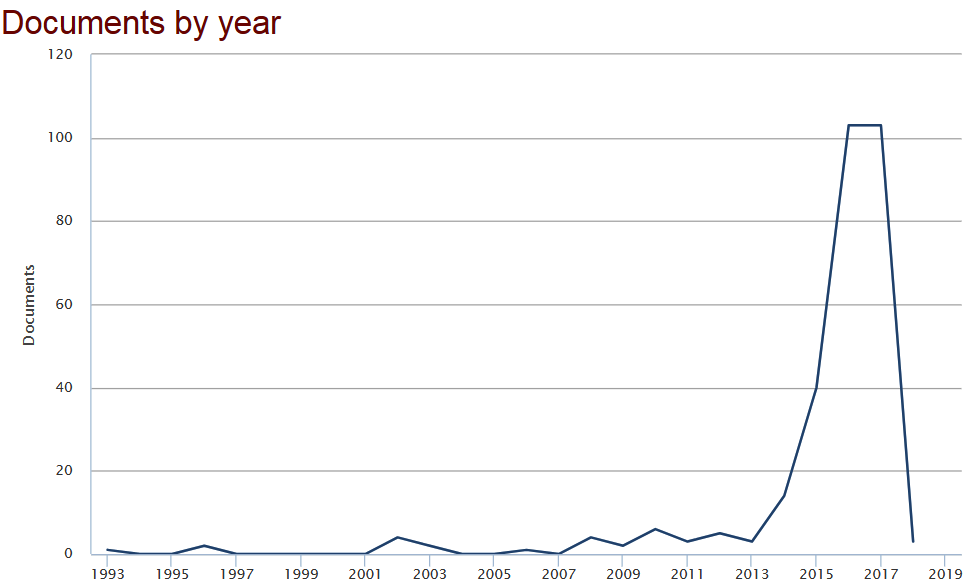
\includegraphics[scale=0.45]{figuras/papersbyyear.png}
\caption{Artigos por ano retornados pela \textit{string} de busca}
\label{fig:papersbyyear}
\end{figure}

\section{Condução da Revisão Sistemática da Literatura}\label{sec:crsl}
\subsection{Primeiro Filtro}
No primeiro filtro foi lido somente o título, resumo e as palavras-chaves do artigo.
A \textit{string} de busca retornou 281 artigos para classificar no primeiro filtro. Foram aceitos 99 (35\%) para o segundo filtro, 3 (1\%) duplicados e 179 (64\%) rejeitados.

Na Seção \ref{sec:stringdebusca}, o autor do protocolo esclarece porque utilizou os seguintes termos na \textit{string} de busca: "long short term memory", "LSTM”, "recurrent neural network" e "RNN", depois do primeiro filtro, realmente comprovou-se que estas técnicas são combinadas com as redes neurais de convolução para classificação de emoção em expressão facial, porém, somente em vídeos ou streaming de imagens. Portanto, os artigos retornados por essas palavras receberam a classificação de rejeitado devido a esta revisão focar em trabalhos com classificação em imagens estática sem streaming. 

\subsection{Segundo Filtro}
Para a realização do segundo filtro foi lido o artigo completo para a extração dos dados e, consequentemente a obtenção dos resultados. No segundo filtro tinham 99 artigos para classificar, onde 34 foram aceitos, 1 duplicados e 64 rejeitados.

\begin{figure}
\centering
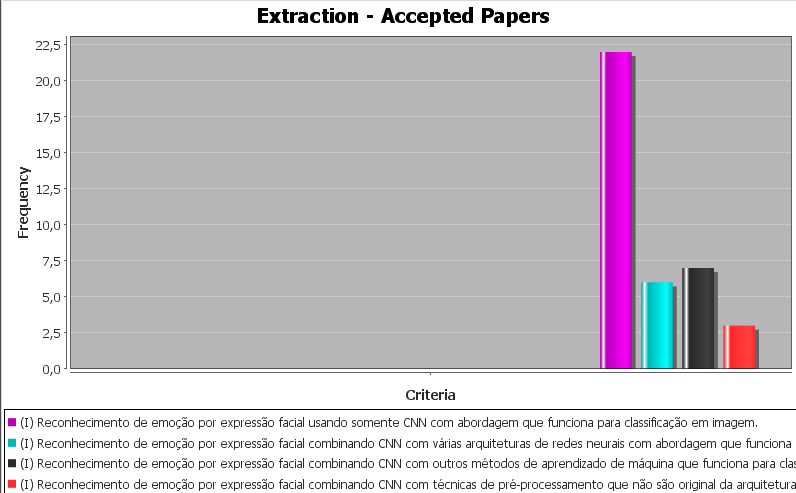
\includegraphics[scale=0.75]{figuras/paperscriteriaaccepted.png}
\caption{Gráfico representando a frequência dos critérios de inclusão para os artigos aceitos do segundo filtro}
\label{fig:papersbyyear}
\end{figure}

\begin{figure}
\centering
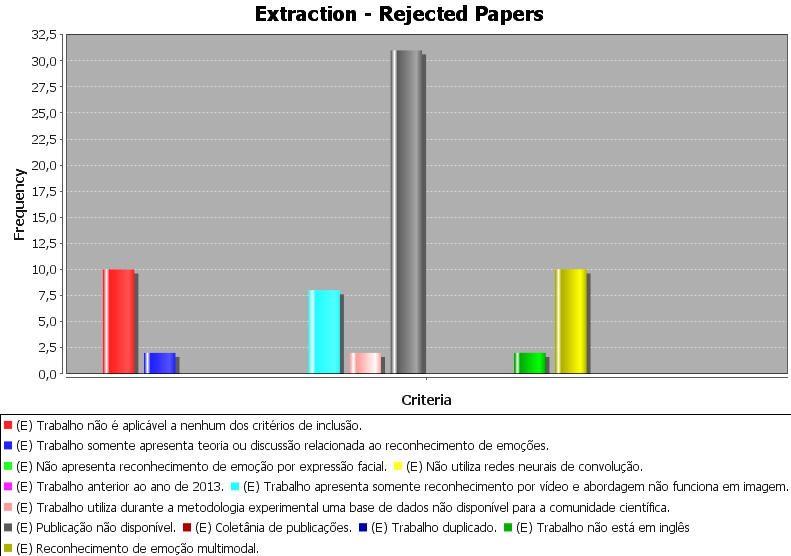
\includegraphics[scale=0.75]{figuras/paperscriteriarejected.png}
\caption{Gráfico representando a frequência dos critérios de exclusão para os artigos rejeitados do segundo filtro}
\label{fig:papersbyyear}
\end{figure}

\section{Resultados}\label{sec:results}
\subsection{Q1: Quais emoções têm sido reconhecidas por meio da expressão facial utilizando redes neurais de convolução?}
As emoções reconhecidas obviamente são as emoções que são representadas e contidas em base de dados, logo são as emoções básicas: neutralidade, felicidade, surpresa, tristeza, raiva, desgosto e medo. Alguns trabalhos como \cite{art8} reconhece também nojo.

\subsection{Q2: Quais tipos de pré-processamento tem sido realizado na imagem?}\label{sec:q2}
Abaixo segue uma lista com o pré-processamento e os trabalhos que fizeram utilização da técnica. 
\begin{itemize}
 \item \textbf{Detector de Face}: Consiste na detecção e recorte da face \citep{art1,art2,art6,art9,art12,art13,art15};
 \item \textbf{Normalização de Brilho (Equalização de histograma)}: Transformada para realce do contraste \citep{art2,art4,art6};
\item \textbf{Normalização Min e Max}: Transformação linear baseada no valor mínimo e máximo da imagem \citep{art4};
\item \textbf{Pontos da Face (pontos geométricos)}: Extração de pontos da face e a distância entre os pontos \citep{art11};
\item \textbf{Escala de Cinza}: Transformação da imagem para escala de cinza \citep{art12};
\item \textbf{Diferença Gaussiana}: Detecta as bordas do objeto, neste caso, evidencia as bordas da face \citep{art6};
\item \textbf{Filtro de Difusão Isotópica}: \citep{art6};
\item \textbf{Normalização DCT}: Transformada discreta do cosseno utilizada em compressão de dados e eventualmente evidenciando informações relevantes da imagem \citep{art6};
\item \textbf{Alinhamento da Face}: Utilização de uma rede neural \textit{autoencoder} para alinhar a face no centro \citep{art4}.
\end{itemize}

\subsection{Q3: Quais arquiteturas de redes neurais de convolução têm sido mais utilizadas?}
A Tabela \ref{arquiteturas} contém as arquiteturas encontradas e os trabalhos que a utilizaram, como podemos verificar a arquitetura AlexNet foi a mais utilizada.

\begin{table}[]\footnotesize
\centering
\begin{tabular}{|c|L|}
\hline
\textbf{Arquitetura} & \textbf{Trabalhos que utilizaram a arquitetura}                                                                                    \\ \hline
AlexNet              & \cite{art1}, \cite{art2}, \cite{art4}, \cite{art7}, \cite{art9}, \cite{art11}, \cite{art13}, \cite{art14}, \cite{art15} \\ \hline
GoogLeNet            & \cite{art10}                                                                                            \\ \hline
VGG                  & \cite{art8}, \cite{art13}                                                                                 \\ \hline
Ensemble             & \cite{art3}, \cite{art5}, \cite{art6}                                                                       \\ \hline
\end{tabular}

\caption{Principais arquiteturas de redes neurais de convolução e os trabalhos que utilizaram}
\label{arquiteturas}

\end{table}

\subsection{Q4: Quais técnicas, métodos e abordagens têm sido utilizados para tratar problemas na imagem como iluminação, rotação, obstrução e escala?}
A principal solução encontrada na literatura foi a ênfase na generalização adequada do aprendizado da rede neural de convolução, isto é, durante a fase de treinamento. Obviamente, as técnicas aplicadas no pré-processamento da imagem (ver Seção \ref{sec:q2}), contribuem para resolver problemas de iluminação por meio da equalização de histograma e de rotação com o alinhamento de face. Entretanto, um achado bastante interessante foi a utilização da técnica de aumento de dados, que consiste durante a fase de treinamento da rede neural de convolução em multiplicar por 10 vezes uma instância (imagem), isto é, gerando 10 novas imagens com pequenos giros da faces, e variações da rotação da pose, escala e iluminação. Acrescendo em 10 vezes o tamanho da base de treinamento, com inserção de variações da imagem resultando em melhor aprendizado da rede.

\subsection{Q5: Quais bases de dados têm sido utilizadas?}
Esta seção tem enfoque nas bases de dados mapeadas para reconhecimento de emoção por expressão facial em uma imagem estática.
Obviamente, é possível encontrar outras base de dados para reconhecimento de emoção que não seja 
por imagem estática, por exemplo, reconhecimento em vídeo, por sensores, em textos e outras.

As bases de dados para reconhecimento de emoção por expressão facial em uma imagem estática tem algo em comum, 
geralmente as amostras de expressões faciais são as mesmas emoções, as chamadas emoções básicas investigadas por \cite{ekman1994}
que são: neutralidade, felicidade, medo, desgosto, raiva, surpresa e tristeza, 
isto significa que são essas as emoções que a comunidade tem reconhecido por expressão facial.
As bases de dados mapeadas podem ser consultadas na Tabela \ref{database}.


\begin{table}\footnotesize
\centering

\begin{tabular}{|c|L|}
\hline
\textbf{Bases de Dados} & \multicolumn{1}{c|}{\textbf{Trabalhos que utilizaram a base para treinamento ou validação}}                                                                                                                  \\ \hline
CK+                    & \cite{art1}, \cite{art2}, \cite{art3}, \cite{art6}, \cite{art7}, \cite{art9}, \cite{art11}, \cite{art12}, \cite{art14}, \cite{art15} \\ \hline
JAFFE                  & \cite{art1}, \cite{art2}, \cite{art3}, \cite{art6}, \cite{art12}                                                                               \\ \hline
FER                    & \cite{art3}, \cite{art4}, \cite{art5}, \cite{art6}, \cite{art7}, \cite{art10}, \cite{art13}, \cite{art14}                                \\ \hline
FER+                   & \cite{art8}                                                                                                                                            \\ \hline
SFEW2.0                & \cite{art6}, \cite{art10}                                                                                                                            \\ \hline
KDEF                   & \cite{art6}                                                                                                                                            \\ \hline
MMI                    & \cite{art11}                                                                                                                                           \\ \hline
CIFE                   & \cite{art15}                                                                                                                                           \\ \hline
EmotiW2015             & \cite{art3}, \cite{art13}                                                                                                                            \\ \hline
\end{tabular}

\caption{Bases de Dados}

\label{table:database}
\end{table}



\subsection{Q6: Quais aplicações podem utilizar o reconhecimento de emoção por expressão facial?}
Há diversas aplicações para o reconhecimento de emoção no mundo real, foi percebido que os pesquisadores de reconhecimento de emoção por expressão facial utilizando rede neural de convolução, ultimamente concentraram seus esforços mais no desenvolvimento de reconhecedores de emoção do que a aplicação em cenários reais, mesmo assim, está aberto para trabalhos futuros inúmeras aplicações desses reconhecedores em diversas áreas, tendo destaque principalmente para: 

\begin{itemize}
\item \textbf{Interação humano computador}: no qual pode ser possível projetar interfaces que se adaptam ao estado emocional do usuário \citep{art1, art3, art5,art8};
\item \textbf{Psiquiatria e cuidados médicos}: 
no qual o reconhecedor de emoção deve monitorar constantemente o paciente ou usuário
fornecendo dados emocionais que podem contribuir para diagnósticos \citep{art1, art3, art12};
\item \textbf{Deficiente visual}: pois pessoas com alto grau de deficiência visual, tem dificuldades na
interação entre pessoas para identificar qual a emoção que as pessoas em volta estão emitindo \citep{art15},;
\item \textbf{Interação humano robô}: fazendo com que robôs estejam habilitados
a interagir com humanos podendo adaptar-se a emoção dos humanos em volta, 
ou até mesmo emitir emoção se aproximando de um humanoide \citep{art6, art14};
\item \textbf{Personagens virtuais e animação}: 
habilitando avatares a copiar expressão humana que podem ser útil para gravações de filmes de animação,
também pode ser usado em aplicações de animação como o popular aplicativo para \textit{smartphone} o \textit{Snapchat},
que identifica a expressão facial do usuário e retorna alguma animação sobrepondo a expressão anteriormente detectada do usuário \citep{art9, art11}.
\end{itemize}

\subsection{Questão Principal: Como reconhecer emoções por meio da expressão facial utilizando redes neurais de convolução em uma imagem estática?}
Diante das fichas de extração, foi percebido que a comunidade explorou diversas estratégias para processar imagens de expressão facial e reconhecer emoção. Algumas abordagens se destacam como: a técnica para aumentar os dados de treinamento e teste, utilizando a técnica flip fazendo até 10 pequenas rotações na imagem, para a CNN aprender a generalizar melhor sendo treinada e testada com uma base de dados maior. A técnica de normalização de brilho (equalização) no pré-processamento, no qual todos os trabalhos que utilizaram esta técnica aumentaram a acurácia do reconhecimento. Também merece destaque o trabalho de \cite{kim2016fusing} em que na sua abordagem, a rede de convolução recebe duas expressões faciais de entrada: a saída de um autoencoder que alinha a face e a imagem original sem alinhamento da face. Esta abordagem melhorou bastante o reconhecimento.

Com relação à arquitetura da rede neural de convolução, quem utilizou um SVM como classificador ao invés de um tradicional softmax obteve maior acurácia. Teve trabalhos que utilizou uma rede com camadas inceptions, hipergrafo, ensembles e concatenação de redes, e todas essas abordagens superaram uma CNN simples. Neste caso, falta um trabalho que possa dizer experimentalmente qual dessas arquiteturas é a melhor. 

Percebemos que existem várias bases de dados disponíveis para a comunidade. As bases de dados que foram mais exploradas foram a CK+, FER2013 e a JAFFE. A base CK+ é composta por expressões faciais capturadas em laboratório, por isso, tem altas taxas de reconhecimento, pois, sua dificuldade para o reconhecimento diminui. Já a base FER2013 foi capturada na “natureza”, por isso sua taxa de reconhecimento é mais baixa sendo uma base bastante complexa para classificação.

Notoriamente os trabalhos utilizam o algoritmo Viola Jones para detecção de face pelo programa OpenCV e fazem o recorte da face excluindo o background. Desta forma, elimina o trabalho da rede em aprender a separar o que é background e o que é face, diminuindo a complexidade da classificação.

Portanto, para reconhecer emoção em uma imagem estática, é necessário o treinamento de uma rede de convolução com um classificador na última camada, com a maior quantidade de dados possível, realizando o recorte da face e utilizar técnicas de normalização na imagem, ocasionando um aumento da taxa de reconhecimento. 

\section{Resumo}\label{sec:consfi}
Neste anexo apresentou uma revisão sistemática da literatura que investigou o estado-da-arte sobre o reconhecimento de emoção por expressão facial por meio de redes neurais de convolução. Verificamos que o tema está bem quente na comunidade, pois, antes de 2013 a String de busca retornou 33 artigos, e em 2013 (3 artigos), 2014 (14 artigos), 2015 (40 artigos), 2016 (103 artigos), 2017 (103 artigos) e 2018 (3 artigos), isso demonstra o crescimento exponencial da área.

Foram mapeadas as principais técnicas de pré-processamento, arquitetura de rede neural de convolução, base de dados, metodologias de treinamento e aplicações do reconhecimento de emoção. A impressão que fica é que a comunidade ainda não está utilizando esses classificadores no mundo real, e o amadurecimento rápido da área depois do surgimento do aprendizado profundo, nos levar acreditar que esses sistemas já estão prontos para ser posto em prática apoiando outras aplicações de interação humano computador, interação humano robô, educação, segurança, computação afetiva e etc.
%%%%%%%%%%%%%%%%%%%%

\chapter{Abordagem Proposta}\label{sec:abordagemproposta}
Neste capítulo é descrita a abordagem proposta para reconhecer emoções por meio da expressão facial e está dividido da seguinte forma. Na Seção \ref{sec:monit} detalha o monitoramento do indivíduo. Na Seção \ref{sec:detect} descreve um módulo de detecção de face e recorte. Na Seção \ref{sec:preproc} aborda as operações de pré-processamento aplicadas na imagem. Na Seção \ref{sec:redeneu} apresenta a atribuição da rede neural de convolução e por fim um resumo do capítulo na Seção \ref{sec:considfi}.  

\section{Monitoramento do Indivíduo}\label{sec:monit}
Um dispositivo que possui uma câmera fotográfica periodicamente está fotografando o indivíduo. Por exemplo, em um ambiente educacional um \textit{tablet} ou \textit{notebook} que executa uma plataforma educacional pode está monitorando o estudante por meio da câmera frontal ou \textit{webcam}. Este cenário configura um ambiente favorecedor para o monitoramento, pois a câmera frontal ou \textit{webcam} sempre está capturando as reações do estudante com ângulo frontal. Em um outro exemplo, destacamos uma aplicação para deficientes visuais onde uma câmera apropriada para \textit{wearables} pode está anexada a roupa do usuário na região peitoral, com intuito de monitorar as reações das pessoas ao redor. Entretanto, neste cenário, ao contrário do anterior, possui maiores desafios do ponto de vista de coleta de dados, pois o usuário que está com a câmera pode movimentar-se capturando imagens tremidas, desfocadas e borradas, além de faces com ângulos variáveis. Lógico que esta questão também é relacionada a qualidade do equipamento, sendo assim, fugindo do foco deste trabalho. A Figura \ref{fig:arquitetura2} ilustra o fluxo da solução proposta. Portanto, enquanto o monitoramento está ocorrendo, as imagens são enviadas para um repositório de entrada de dados.

\section{Detecção de Face e Recorte}\label{sec:detect}
Este procedimento consiste na detecção de todas as faces de uma imagem por meio do algoritmo Viola Jones (veja Seção \ref{sec:detecfacialviola}). Primeiramente, uma imagem é consumida do repositório de entrada de dados. A detecção consiste na geração de um conjunto de coordenadas que possibilita o desenho de um retângulo indicando a localização da face. Vale ressaltar que esta atividade possui complexidade moderada, pois uma imagem oriunda de cenários reais contém vários objetos com diferentes geometrias, inclusive podendo assemelhar-se a uma face ocasionando a geração de falsos positivos. Logo após a detecção de face, é realizada o recorte da mesma indicada pelo conjunto de coordenadas definidas pela etapa anterior, tal atividade é valorosa para exclusão do \textit{background}. Desta forma, somente a face recortada segue no \textit{workflow} reduzindo a complexidade do problema, pois não há necessidade do classificador aprender a separar o \textit{background} da face. Posteriormente, ao recorte da face, a imagem original que deve está com uma face recortada é mantida para nova averiguação de recorte de face. Caso exista outras faces na imagem, este processo é repetido até não existir mais faces para recortar. Obviamente caso seja enviada uma imagem para a etapa de detecção e recorte que não contém uma face (e.g. imagem de um avião) o processo é automaticamente encerrado, pois se não há uma face para detectar, logo não há uma expressão facial emocional para reconhecer. 

\section{Pré-Processamento}\label{sec:preproc}
Uma face recortada é recebida pelo módulo de Pré-processamento. Nesta etapa, operações de pré-processamento são aplicadas com a finalidade de enaltecer as características próprias de cada expressões faciais, com intuito de preparar a imagem para a classificação facilitando a diferenciação das emoções. A Figura \ref{fig:preprocessingfluxo} mostra o fluxo desta etapa. Adicionalmente, uma função de redimensionamento é chamada para transformar a imagem em uma escala de 60x60 \textit{pixels}. Neste trabalho, consideramos que a imagem é colorida, portanto a mesma possui 3 canais denominados RGB (do inglês: Red, Green e Blue), então a imagem resultante possui 10.800 características que pode ser calculada por \textit{Qtd_Caracteristica = N_Pixels_X * N_Pixels_Y * N_Canais}. 
%Após o redimensionamento, é realizado a normalização da imagem dividindo cada \textit{pixel} por 255, isto é, o valor máximo que um \textit{pixel} pode possuir, ocorrendo a normalização dos valores dos \textit{pixels} para o intervalo de 0 a 1. 

O problema visualizado por esta proposta consiste em classificar emoções em qualquer ambiente. Obviamente a variação do ambiente acarreta em diferentes níveis de intensidade da luz, ocorrendo a perda de características importantes da face que diferenciam as emoções, seja por excesso ou ausência de luz. Vale destacar que esta proposta é baseada principalmente em redes neurais de convolução que originalmente possui vários filtros de pré-processamento. Entretanto, a literatura tem mostrado que filtros clássicos aplicados antes da inserção de uma imagem em redes neurais tem sido eficazes na eliminação de ruídos, principalmente aqueles relacionados a iluminação e brilho \citep{art2,art4,art6}. Portanto, as técnicas de normalização de brilho e iluminação são parte da etapa de pré-processamento agregando valor para a solução minimizar a sensibilidade relacionada a variação de luz do ambiente. Assim, a imagem normalizada por filtros de correção de iluminação ressaltará melhor os traços faciais, além da imagem transformada está com maior nitidez para a continuação do \textit{workflow}.

Este trabalho também foca em minimizar os efeitos negativos de rotações da face e variação da pose para treinamento e classificação. Rotações e poses com elevado grau dificultam a classificação e minimizam o aprendizado caso a base de treino tenha muita imagem com face rotacionada. Por isso, no pré-processamento é feito o alinhamento da face. Este alinhamento é por meio da localização de três pontos: o canto do olho direito, o canto do olho esquerdo e um ponto central do nariz. Desta forma, esses três pontos formam um triângulo, sendo possível rotacionar a imagem até que não haja uma inclinação na linha dos olhos orientada pelo triângulo. Após o alinhamento, é realizado a normalização da imagem dividindo cada \textit{pixel} por 255, isto é, o valor máximo que um \textit{pixel} pode possuir. Resultando na normalização dos valores dos \textit{pixels} entre o intervalo de 0 a 1. 

\begin{figure}
\centering
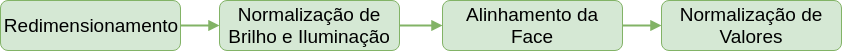
\includegraphics[scale=0.5]{figuras/PreProcessamentoMestrado.png}
\caption{Pré-Processamento fluxo}
\label{fig:preprocessingfluxo}
\end{figure}



\section{Rede Neural de Convolução}\label{sec:redeneu}
A rede neural de convolução é a parte central e com importante contribuição nesta abordagem. Por meio dela, durante o treinamento as imagens são processadas a fim de aprender os contornos, padrões, formas e características relevantes para a classificação. Além disso, funções são aplicadas para redução de dimensionalidade, extração de características e normalização, ocasionando que a rede não seja sensível a rotações, posições e escala da imagem. Tais aptidões são requisitos para um classificador de imagens ser usado em cenários reais. Apesar de a rede neural ter embutida normalizações e rotações internas, vale a pena realizar as operações da Seção \ref{sec:preproc}, pois são técnicas selecionadas especialmente para o problema de faces, e além disso, a comunidade científica tem descoberto que combinar o processamento interno da rede neural de convolução com outros processamentos externos alcançam os melhores resultados. Vale ressaltar que um desempenho satisfatório da rede neural de convolução, assim como de qualquer algoritmo supervisionado de aprendizagem de máquina, está estritamente relacionado ao processo de treinamento e validação do modelo.    

\subsection{Treinamento}
O treinamento da rede neural de convolução é parte fundamental para o classificador de emoção funcionar bem. Nesta etapa, é buscada a generalização satisfatória e adquirir aprendizado suficiente para funcionar em variados ambientes. Para isso, neste trabalho, o treinamento é apoiada pela técnica de aumento de dados com intuito de maximizar a generalização do aprendizado durante o treinamento. O aumento de dados consiste na multiplicação das imagens em tempo dinâmico modificando levemente a imagem e seu contexto, realizando alterações nas imagens aplicando zoom, rotações, \textit{blur}, \textit{shear}, diferentes níveis de contraste e dentre outros. Com o propósito de estimular maiores taxas de aprendizado e generalização, pois, assim, a rede neural observa a região de interesse que são as expressões faciais emocionais em diferentes cenários, sendo assim, gerando modelos capazes de classificar emoções em contextos variados. 

\subsection{Extração de Características e Classificação}
Em problemas de classificação de imagem, uma etapa fundamental é a extração de caraterísticas. Sendo responsável em retirar de uma entrada de dados as principais informações para enviar a um classificador, e assim, determinar a classe. Na rede neural de convolução, a extração de característica é um procedimento que procura identificar as zonas da imagem que são mais relevantes para a separação do problema, isto é, classificar uma expressão facial (\textit{e.g} o sorriso humano é uma característica indicadora para a emoção felicidade). Este processo funciona com as camadas de convolução da rede operando sobre a imagem de entrada ressaltando todos os contornos e com a camada de \textit{pooling} aplicando redução de dimensionalidade. Algumas camadas de convolução são especialistas na extração dos padrões verticais, outras nos horizontais, até que um conjunto de características são extraídas para enviar a um classificador.

%\textit{softmax} classificar estimando a probabilidade para cada emoção.
A rede neural de convolução recebe a imagem pré-processada de uma face para classificá-la estimando a probabilidade para cada emoção: neutralidade, raiva, felicidade, tristeza, desprezo, medo e surpresa, de acordo com as caraterísticas extraídas da imagem.  

%contornos, bordas, linhas, horinzontais, verticais
%Produto de probabilidades Naive Bayes

\begin{figure}
\centering
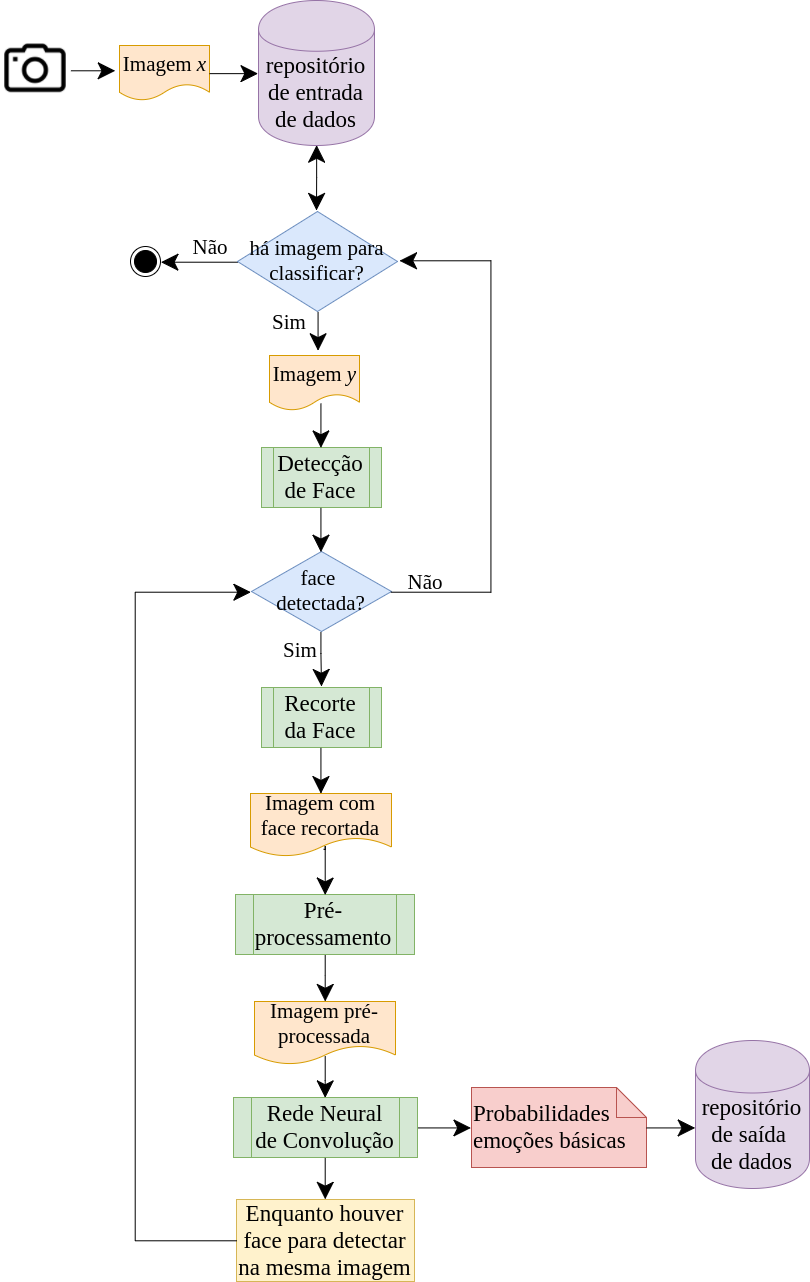
\includegraphics[scale=0.45]{figuras/arquitetura.png}
\caption{Solução Proposta}
\label{fig:arquitetura2}
\end{figure}

     

\section{Resumo}\label{sec:considfi}
%imagens gerais
%LUTE LUTE LUTE LUTE GO FIGHT GO FIGHT YOU CAN ONLY DEPENDS YOU SON OF BEATCH

\chapter{Resultados Parciais}\label{sec:resultados}
Neste capítulo serão apresentados os resultados parciais. Na Seção \ref{sec:prova} está descrito um artigo publicado no Simpósio Brasileiro de Informática na Educação (SBIE) como parte de resultados parciais e que nortearam esta proposta. Na Seção \ref{sec:reconhecedor} contém a evolução do artigo anteriormente citado e a implementação de um reconhecedor utilizando redes neurais de convolução, obviamente ainda é uma versão preliminar do reconhecedor que esta proposta pretende fornecer como contribuição e enquanto a Seção \ref{sec:considera} o resumo deste capítulo. 

\section{Prova de Conceito}\label{sec:prova}
Inicialmente, realizamos uma prova de conceito para nortear o andamento deste projeto. Como resultado esta prova de conceito foi publicada no Simpósio Brasileiro de Informática na Educação (SBIE) 2017 \citep{cruz2017framework}. Nesta prova de conceito foi utilizada a API da \textit{Microsoft Cognitives Services} como reconhecedor de emoções, esta experiência foi bastante proveitosa pois, foi possível ponderar as vantagens e desvantagens desta API, e assim, podemos nortear a construção do nosso próprio reconhecedor. Além disso, mostramos que é possível utilizar computadores para reconhecer emoções em tempo real, de forma automática, com confiança aceitável em cenários de uso real. Como foi visto na revisão sistemática (ver Capítulo \ref{sec:revisaosistematica}), os pesquisadores da área de aprendizado profundo ainda não estão colocando esses reconhecedores no mundo real, desta forma, a utilização em cenários reais passa a ser um ponto de contribuição deste trabalho por pretender utilizar nesses cenários. Visto que, funcionar no cenário real, não é uma tarefa trivial, o reconhecedor deve alcançar uma excelente taxa de generalização, há muitas variações da face e do ambiente dificultando o reconhecimento.  

\subsection{Resumo}
Neste artigo \citep{cruz2017framework}, propomos um \textit{framework} para detectar estados emocionais de alunos baseado em reconhecimento de expressões faciais no contexto das plataformas digitais. Analisamos e discutimos o uso de correlação e entropia entre os estados emocionais dos estudantes e o desempenho durante uma avaliação de múltipla escolha. Realizamos um experimento com 27 estudantes e elaboramos um teste composto de 40 perguntas. Na análise, correlacionamos os estados emocionais de neutralidade, tristeza, felicidade, raiva, desgosto, medo, desprezo e surpresa com o desempenho no teste. Concluímos que as questões que ocorreram maior variabilidade das emoções tinham também as maiores proporções de acertos.

\subsection{Objetivos}
O artigo \citep{cruz2017framework} tem como objetivo: (i) propor uma arquitetura de detecção automática de emoções para ambientes educacionais digitais por meio de reconhecimento automático de expressões faciais, utilizando processamento digital de imagens, de modo a tornar possível a obtenção de dados emocionais dos alunos durante o processo de aprendizagem, e (ii) analisar por meio de estatística descritiva um estudo de caso com dados obtidos a partir desta arquitetura. Esta análise pretende investigar e medir correlações entre as emoções e o desempenho obtido nas questões, levantando hipóteses relevantes sobre a relação entre os estados emocionais e o desempenho, o qual é relevante para sistemas de recomendações, tutores inteligentes e heurísticas em geral, que se interagem de forma dinâmica com as necessidades de aprendizado de cada aluno

\subsection{Método Proposto}
A arquitetura proposta na Figura \ref{fig:metproposto} é formada pelos seguintes componentes: (i) uma plataforma educacional digital executada, por exemplo, em um tablet com câmera frontal que possibilite a coleta de imagens das expressões faciais e das atividades dos alunos, relacionadas com a seleção das respostas e a navegação entre os diferentes objetos de aprendizagem; (ii) um classificador de emoções que recebe como entrada as imagens das expressões faciais e retorna um vetor com as probabilidades a posteriori das seguintes emoções: neutralidade, surpresa, felicidade, tristeza, desprezo, raiva, medo e desgosto; e (iii) um conjunto de métodos de estatística descritiva para realizar diversas análises úteis para: inferências, heurísticas, sistemas de recomendações, tutores inteligentes e inclusive para auxiliar o professor na tomada de decisões referentes às dificuldades de aprendizagem de cada aluno. A arquitetura proposta pode ser usada em tempo real, tanto em ambientes presenciais como à distância, possibilitando o cruzamento dos estados emocionais com a interação na plataforma.

\begin{figure}
\centering
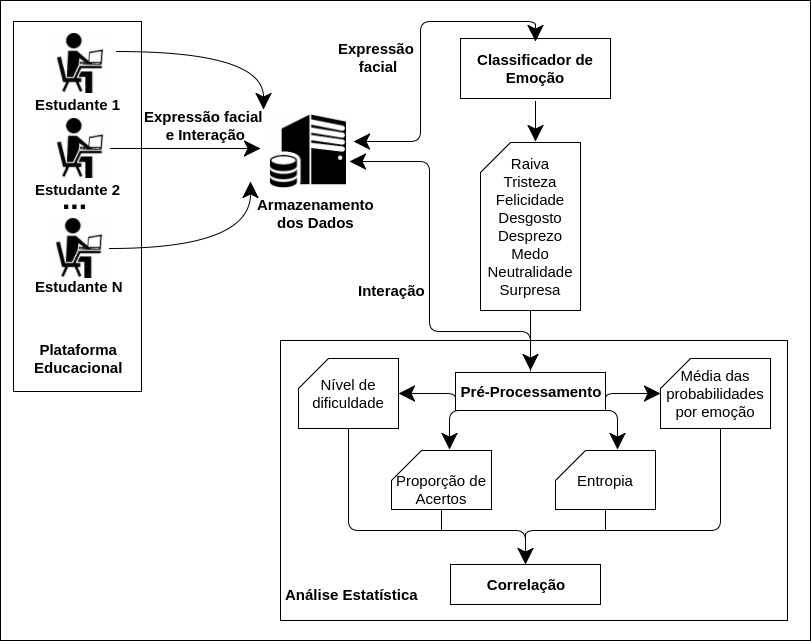
\includegraphics[scale=0.5]{figuras/diagrama.png}
\caption{Método Proposto}
\label{fig:metproposto}
\end{figure}

\subsubsection{Plataforma Educacional}
A plataforma educacional deve possuir um módulo coletor de dados que armazene continuamente os eventos da interação do estudante, tais como, a seleção das questões e suas respectivas respostas, e a identificação de todos os itens presentes na interface como botões, caixa de texto, opções de seleções e outros, assim como, a captura contínua da expressão facial do estudante.

Estes dados são armazenados para tornar possível diferentes análises, tais como: qual foi a emoção predominante na questão que os alunos mais erraram? Na questão que houve mais troca de respostas qual foi a emoção predominante? Qual foi a emoção predominante no grupo de alunos que mais erraram as questões? Quais são as emoções causadas pela variação da dificuldade das questões? Isto pode ser um caminho para inferir a confusão via expressão facial, onde \cite{d2013beyon}, em alguns estudos de casos, concluiu que a confusão, tédio, curiosidade, engajamento, frustração e satisfação ocorrem cinco vezes mais do que as emoções básicas no âmbito educacional.

\subsubsection{Classificador de Emoção}
O classificador de emoção tem a função de identificar nas imagens as expressões faciais de um estudante e atribuir um rótulo a cada imagem. Estes rótulos podem ser: neutralidade, raiva, felicidade, tristeza, desgosto, desprezo, medo e surpresa, como mencionado por \cite{ekman1994}, que são as emoções básicas capazes de ser reconhecidas dada uma expressão facial.

O classificador utilizado está descrito na Seção \ref{sec:plan}, e usufrui de técnicas de aprendizagem de máquina, mais especificamente de aprendizagem profunda em redes neurais pela arquitetura \textit{Convolutional Neural Network} (CNN), que tem sido o estado da
arte para este fim.

A saída do classificador de emoção para cada imagem recebida é um vetor de probabilidades que contém a probabilidade de cada emoção detectada na imagem \textit{i.e.: P=\{p\textsubscript{1},p\textsubscript{2},..,p\textsubscript{n}\}}, onde \textit{p\textsubscript{n}} representa a probabilidade a posteriori da detecção da n-ésima emoção. Uma propriedade é que a soma das probabilidades é igual a 1, e que a maior probabilidade presente no vetor corresponde ao rótulo final da emoção detectada na imagem, ou seja, a sua classificação \textit{e.g.: emoção = max(P)}.

\subsubsection{Análise Estatística}
Este componente contém outros subcomponentes que realizam análises acerca do desempenho e das emoções do estudante por meio da correlação de Pearson. Todos os subcomponentes recebem como entrada tanto os cliques de interação do estudante com a plataforma, como as classificações das expressões faciais. Desta forma, são recuperadas todas as instâncias necessárias para a realização do cruzamento da interação da plataforma com a emoção detectada, a fim de obter o coeficiente de correlação.

Um pré-processamento dos dados é executado antes da análise, onde é organizada a coleção de dados por questão, isto é, a reunião de todas as instâncias de todos os alunos com respeito a uma determinada questão e, desta forma, são agrupados a interação com a plataforma e os dados das classificações de emoções por questão. O
pré-processamento produz as seguintes informações para cada questão:

\begin{itemize}
 \item a média das probabilidades para cada emoção, incluindo todos os alunos;
 \item o nível de dificuldade;
 \item a proporção de acertos, por exemplo, se a metade dos alunos acertaram, então a
proporção é 50\%; e
 \item a entropia das emoções, que mede a dispersão das probabilidades das emoções
detectadas, isto é, caso em uma questão haja várias emoções diferentes e estejam
distribuídas uniformemente, a entropia será maior.
\end{itemize}
Todos esses dados pré-processados entram no componente de análise estatística,
e a sua saída pode ser útil para traçar um perfil emocional do estudante e da turma
mediante as correlações identificadas.

\subsection{Metodologia Experimental}
Um experimento foi realizado com 27 alunos do Ensino Médio de uma escola de tempo integral que farão o Exame Nacional do Ensino Médio (ENEM) 2017. O experimento consistiu em um simulado do exame contendo 40 questões de múltipla escolha.

\subsubsection{Planejamento}\label{sec:plan}
Adotamos uma plataforma educacional que permite a execução de questionários de múltipla escolha, coleta de cliques efetuados pelo estudante, captura automática de foto via câmera frontal do dispositivo, seja por \textit{tablet}, \textit{smartphone} ou \textit{notebook}. Os assuntos escolhidos foram: matemática, língua portuguesa, química, raciocínio lógico, geografia e história. O simulado teve duração de duas horas e cada questão possuía dois níveis de dificuldade (fácil ou difícil), além de ter cinco respostas alternativas.

Para o componente classificador, selecionamos a API da \textit{Microsoft Cognitives Services}, justamente por classificar bem emoções como neutralidade, felicidade e tristeza. Acreditamos que, no contexto da educação, uma emoção bastante comum é a neutralidade, pelo fato da expressão facial do estado de concentração se assemelhar bastante com a expressão facial de neutralidade reconhecida por esta API. Constatamos que estudantes quando estão pensando, estão concentrados, emitindo poucas movimentações intensas e variações de suas expressões faciais, assemelhando-se com a expressão de neutralidade.

\subsubsection{Execução}
A seleção dos estudantes para participar do experimento ocorreu voluntariamente. O grupo final formado foi heterogêneo, onde 53\% consideravam até o momento seu desempenho na escola como bom ou ótimo e, 47\% como regular ou ruim; além disso, 30\% deles consideravam a sua preparação para o vestibular como boa ou ótima e, 70\% como regular ou fraca. Os alunos selecionados são de turmas diferentes.

\subsection{Resultados e Discussões}
Inicialmente, obtemos os seguintes atributos calculados como os valores médios por questão, utilizando os dados coletados dos vinte e sete alunos: (i) a proporção de acertos; (ii) o nível de dificuldade; (iii) a média das probabilidades para cada emoção detectada; e (iv) a entropia por questão. Assim, obtemos um total de onze atributos (resumidos na Tabela \ref{tabelaArti}), onde cada um deles é representado por uma variável aleatória com quarenta valores.

Posteriormente, aplicamos a correlação de Pearson para analisar se há qualquer grau de correlação entre os pares dos atributos mencionados. A Tabela \ref{tabelaArti} apresenta a correlação entre a média das probabilidades de cada emoção com o nível de dificuldade e a proporção de acertos. Os principais resultados estão destacados em negrito.

Como podemos verificar na Tabela \ref{tabelaArti}, a expressão facial neutra possui uma correlação negativa com a proporção de acertos dos alunos (segunda coluna da Tabela \ref{tabelaArti}). Isto indica que estimular emoções diferentes da neutralidade durante a avaliação favorece o desempenho dos alunos. Um segundo indicativo de que isto ocorre, é dado pela correlação positiva entre o desprezo e a felicidade com a proporção de acertos e, de forma discreta, também ocorre com tristeza, surpresa e medo.

A entropia é calculada a partir do valor das probabilidades das emoções detectadas. Logo, percebemos que quando a neutralidade baixa, a entropia aumenta, o que significa que outras emoções estão sendo detectadas com maior probabilidade, ocorrendo a dispersão dos estados emocionais. Portanto, o fato de existir uma correlação positiva entre o aumento da entropia e a proporção de acertos reforça a observação constatada no parágrafo anterior. Adicionalmente, descobrimos que a emoção mais frequente foi a neutralidade, devido aos alunos passarem a maior parte do tempo concentrados analisando as questões para a busca de soluções. Assim, quando o nível de dificuldade da questão aumenta, a neutralidade também aumenta, isto pode ser um indício de que questões mais difíceis tem tendências de exigir maiores níveis de concentração do estudante.

Podemos considerar a hipótese de que, quando o estudante está respondendo uma questão, ao selecionar uma resposta, o mesmo tem uma percepção se acertou ou errou e, nesse momento, há possibilidade de emitir emoções positivas como felicidade e surpresa, ou emoções negativas como tristeza ou desprezo. Portanto, há uma variação dos estados emocionais durante o tempo de resposta de cada questão que deve ser considerado como um problema de mudança de estados. Este resultado é reforçado por
questões que ocasionaram maior entropia, ou seja, quanto maior a dispersão das emoções, maior é o índice de proporções de acertos.

A emoção desprezo aumenta a medida que as questões têm maiores proporções de acertos, isto pode ser explicado, pela mudança de estados durante o tempo de resposta de cada questão ou pelo fato da expressão facial de desprezo se assemelhar com a expressão facial de felicidade. Neste caso, é bem provável estar ocorrendo confusão por parte do classificador em diferenciar felicidade e desprezo.

\begin{table}[]\footnotesize
\centering
\caption{Resultado​ ​da​ ​correla\c{c}\~ao​ ​de​ ​Pearson​ ​para​ ​cada​ ​emo\c{c}\~ao​ ​detectada
e​ ​a​ ​entropia​ ​contra​ ​os​ ​atributos​ ​das​ ​quest\~oes}
\label{tabelaArti}
\begin{tabular}{|c|c|c|}
\hline
                      & \textbf{Nível de Dificuldade} & \textbf{Proporção de Acertos} \\ \hline
\textbf{Tristeza}     & \textbf{-0.33}                & 0.27                          \\ \hline
\textbf{Neutralidade} & \textbf{0.36}                 & \textbf{-0.48}                \\ \hline
\textbf{Desprezo}     & -0.15                         & \textbf{0.30}                 \\ \hline
Desgosto              & -0.13                         & 0.07                          \\ \hline
Raiva                 & -0.14                         & -0.08                         \\ \hline
Surpresa              & 0.07                          & 0.24                          \\ \hline
Medo                  & -0.06                         & 0.14                          \\ \hline
\textbf{Felicidade}   & -0.14                         & \textbf{0.31}                 \\ \hline
\textbf{Entropia}     & -0.12                         & \textbf{0.36}                 \\ \hline
\end{tabular}
\end{table}



\subsection{Considerações Finais}
Nesta prova de conceito, propomos uma arquitetura de reconhecimento de emoções de alunos por meio de sua expressão facial para plataformas educacionais, a partir da qual realizou-se um estudo de caso com a coleta de dados reais de estados emocionais obtidos por meio da própria arquitetura. Como resultado principal apontamos que as questões onde ocorreram diferentes emoções, são as questões onde há maiores proporções de acertos.

Tanto a arquitetura para o reconhecimento de estados emocionais, como a
realização de análises de estados emocionais de estudantes, são úteis para a implementação de tutores inteligentes e sistemas de recomendações que possam fornecer personalização mais precisa do conteúdo para cada aluno levando em consideração seus estados emocionais. É importante identificar os casos diferentes da expressão neutra, justamente por serem menos frequentes podendo indicar alguma oportunidade de um tutor inteligente atuar.

Como trabalho futuro, pretendemos investigar a mudança temporal dos estados emocionais do estudante, mediante a estímulos produzidos por diferentes objetos de aprendizagem durante uma aula. Também, a implementação de uma heurística que considera o estado emocional do estudante para fornecer ajuda sob demanda com a intenção de aumentar o engajamento e o desempenho durante uma aula.

Finalmente, percebe-se que o \textit{framework} para classificação automática de emoções a partir de imagens necessita de um maior volume de dados, para reduzir eventuais erros de classificação, e permitir a classificação de novos tipos de emoções. Portanto, está nos nossos planos investigar alternativas para amenizar erros de classificação e melhorar a acurácia do \textit{framework}.

\section{Reconhecedor de Emoção}\label{sec:reconhecedor}
Foi iniciado o desenvolvimento do reconhecedor de emoção, visto que, para trabalhar com redes profundas, especificamente com as redes neurais de convolução é necessário dispor de grandes quantidades de recursos computacionais relacionadas a memória e a processamento. Por isso, como ponto de partida optamos por uma arquitetura reduzida da AlexNet ilustrada na Figura \ref{fig:implementadaarquitetura}, utilizamos esta arquitetura para treinar e gerar um modelo para classificar emoções em expressões faciais.

Para gerar o modelo utilizamos a base de dados \textit{FER-2013} tanto para treinar como para validar, esta base é bastante utilizada pela literatura e contém 28709 imagens de expressão facial com as seguintes emoções (classes): raiva, desgosto, medo, felicidade, tristeza, surpresa e neutralidade. Foi utilizado 2/3 da base de dados para treinamento e o restante para validação. A rede foi treinada por 140 épocas e alcançou os seguintes resultados expresso na matriz de confusão na Figura \ref{fig:confusionmatrix}. Para implementação da rede neural de convolução foi utilizado o \textit{framework Tensorflow} (\url{https://www.tensorflow.org/}), em um computador com a seguinte configuração: \textit{GPU NVIDIA GEFORCE 930}, \textit{Intel Core-i7} e \textit{16 GB de RAM DDR4}. 

Seguimos a abordagem proposta na Seção \ref{sec:abordagemproposta}, e como detector de face utilizamos o Viola Jones implementado pela biblioteca \textit{OpenCV 3.0} (\url{https://opencv-python-tutroals.readthedocs.io/en/latest/}), nesta implementação diferentemente da abordagem proposta, foi realizado uma normalização transformando a imagem em escala de cinza (ver Figura \ref{fig:implementadaarquitetura}). Esta implementação foi anteriormente a revisão sistemática da literatura, a revisão mostrou que as redes neurais de convolução sabem lidar com a imagem colorida, então, é desnecessário transformar em escala de cinza, no entanto, pode ser interessante em uma configuração de experimento verificar qual a melhor proposta com a imagem colorida ou em escala de cinza. 

\begin{figure}
\centering
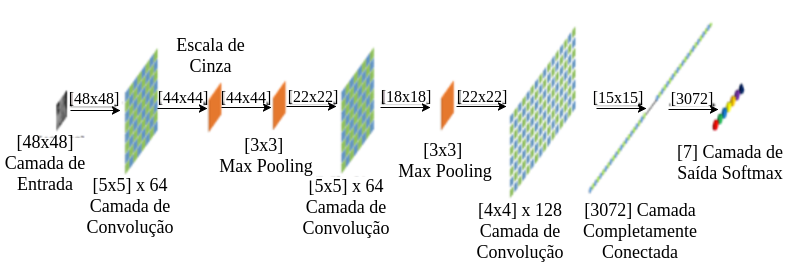
\includegraphics[scale=0.57]{figuras/arquiteturaimplementada.png}
\caption{Arquitetura Implementada de Rede Neural de Convolução}
\label{fig:implementadaarquitetura}
\end{figure}


\begin{figure}
\centering
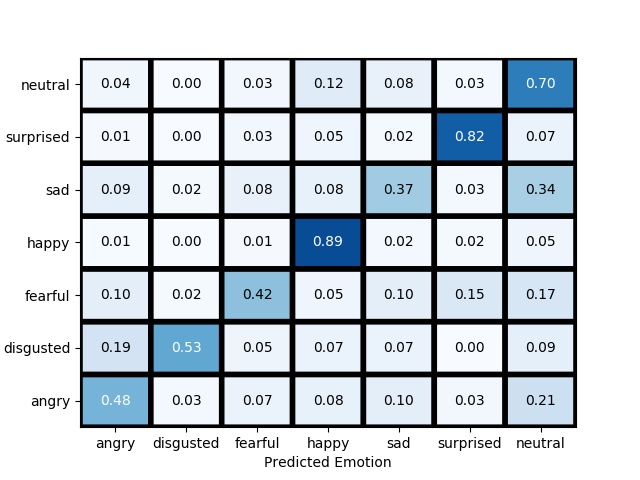
\includegraphics[scale=0.8]{figuras/confusion-matrix-75split-140epo.png}
\caption{Matriz de Confusão com 140 épocas de treinamento}
\label{fig:confusionmatrix}
\end{figure}

\section{Resumo}\label{sec:considera}
Foi possível verificar que o reconhecedor de emoção tem muita aplicação, iniciamos nossa aplicação no cenário real em uma prova de conceito na área de educação, no qual há muitas utilidades. Esta prova de conceito nos deu norte para a evolução desta proposta. Consequentemente foi iniciado o desenvolvimento do reconhecedor que esta proposta pretende gerar como contribuição. Há muitos trabalhos futuros, principalmente combinar as diversas técnicas de pré-processamento com as diversas arquiteturas de RNC juntamente com as bases de dados. A área de aprendizagem de máquina costuma ser bastante experimental e aparentemente temos bastante configuração de experimento para testar, até encontrar a melhor taxa de aprendizado da RNC.

\chapter{Considerações Finais}\label{sec:conclusao}
Neste trabalho, foi apresentado uma abordagem para reconhecer emoção por meio da expressão facial utilizando redes neurais de convolução. O diferencial desta abordagem é reunir os principais elementos identificados na literatura para reconhecer emoções. Além disso, este trabalho pretende fornecer uma solução para reconhecer emoções em computação embarcada e em nuvem.     

Uma prova de conceito foi aplicada para verificar a viabilidade do reconhecimento de emoção por expressão facial. Nesta prova de conceito, um serviço em nuvem foi utilizado para reconhecer as emoções. O foco foi monitorar estudantes por meio da captura de imagens em tempo real, enquanto faziam um teste escolar com questões de múltipla escolha. Foram correlacionadas as emoções com o desempenho no teste. Portanto, como resultado principal identificamos que as questões onde ocorreram diferentes emoções, foram as questões que tiveram maiores proporções de acertos.  

Adicionalmente, para gerar nosso próprio reconhecedor de emoção, um estudo experimental foi conduzido com intuito de avaliar três arquiteturas de redes neurais de convolução: AlexNet, Inception-V3 e ResNet-34. Os resultados apontaram que a ResNet-34 obteve as melhores taxas de acurácia, precisão, revocação e f1-score. As imagens utilizadas no estudo foram provenientes da natureza e laboratório. Concluímos que um método treinado pelas imagens da natureza não influenciam negativamente para reconhecer imagens laboratoriais. Em contrapartida, um método treinado com as imagens laboratoriais não consegue reconhecer emoções no contexto da natureza.


\section{Limitações do Trabalho}
Este trabalho tem como objetivo reconhecer emoções humanas por meio da expressão facial. Todavia, os trabalhos de \cite{darwin1965expression} e \cite{ekman1994} apontaram que somente o grupo das emoções básicas (raiva, alegria, tristeza, desgosto, medo e surpresa) são emitidas por meio da expressão facial. Portanto, este trabalho tem possibilidades de reconhecer exclusivamente as emoções básicas. 

\section{Trabalhos Futuros}
\begin{itemize}
 \item \textbf{Analisar sequência de imagens}: Atualmente, a abordagem analisa somente uma imagem para reconhecer as emoções. Desta forma, está sendo ignorada a característica temporal e apenas uma imagem é considerada para definir as emoções. Integrar uma sequência de imagens, na forma de uma série temporal, pode ser relevante para melhorar o reconhecimento, justamente por analisar um conjunto de imagens amostrada em uma fração de tempo para definir as emoções. 
 \item \textbf{Avaliar experimentalmente outros classificadores}: O \textit{softmax} foi o único classificador adotado no estudo realizado. É interessante avaliar o desempenho de outros classificadores analisando diferentes famílias:  SVM (funcional), Gaussiana (probabilística) e RandomForest (ensemble de árvores de decisões).
 \item \textbf{Implementar e avaliar a MobileNet}: A MobileNet é a arquitetura de rede neural de convolução apropriada para sistemas embarcados. É necessário um estudo para parametrizar a MobileNet, mensurar o consumo de recursos computacionais e, além disso, definir as especificações mínimas de hardware para a instalação e funcionamento.  
 \item \textbf{Desenvolver e avaliar o componente de pré-processamento}: As técnicas de alinhamento de face, normalização de iluminação e aumento de dados, devem ser implementadas. É interessante um estudo para avaliar a contribuição e o impacto dessas técnicas. Principalmente, no cenário das imagens oriundas da natureza, em que nesse contexto, o método proposto não obteve bons resultados.
 \item \textbf{Avaliar em cenários de uso reais}: Nos seguintes cenários pretendemos aplicar a solução: na educação ou em tecnologia assistiva para deficientes visuais. Na educação é útil para auxiliar sistemas inteligentes que interagem com aluno de acordo com a emoção do mesmo. Na tecnologia assistiva pode auxiliar deficientes visuais que tem dificuldades em reconhecer emoção, inclusive este tipo de aplicação abre um campo desafiador para a interação humano computador.
 
\end{itemize}


%\chapter{Cronograma}\label{sec:cronograma}

O cronograma está descrito na Tabela \ref{cronog}.

\begin{table}[]\footnotesize
\centering
\caption{Cronograma de Atividades}
\label{cronog}
\begin{tabular}{|A|c|c|c|c|c|c|c|c|c|c|c|c|}
\hline
                                                     & \multicolumn{12}{c|}{\textbf{Ano 2018}}                                                                                                                                           \\ \hline
\textbf{Atividades}                                  & \textbf{jan} & \textbf{fev} & \textbf{mar} & \textbf{abr} & \textbf{mai} & \textbf{jun} & \textbf{jul} & \textbf{ago} & \textbf{set} & \textbf{out} & \textbf{nov} & \textbf{dez} \\ \hline
Implementação do componente de pré-processamento     & x            & x            &              &              &              &              &              &              &              &              &              &              \\ \hline
Implementação da arquitetura GoogLeNet               &              & x            & x            &              &              &              &              &              &              &              &              &              \\ \hline
Implementação da arquitetura VGG                     &              &              & x            &              &              &              &              &              &              &              &              &              \\ \hline
Implementação da arquitetura Ensemble                &              &              & x            & x            &              &              &              &              &              &              &              &              \\ \hline
Download das bases de dados                          & x            & x            &              &              &              &              &              &              &              &              &              &              \\ \hline
Planejamento experimental das RNCs                   &              &              &              & x            &              &              &              &              &              &              &              &              \\ \hline
Treinamento das RNCs                                 &              &              &              &              & x            & x            & x            &              &              &              &              &              \\ \hline
Avaliação experimental das RNCs                      &              &              &              &              &              &              &              & x            &              &              &              &              \\ \hline
Planejamento experimental para cenários de uso reais &              &              &              &              &              &              &              & x            &              &              &              &              \\ \hline
Execução do experimento para cenários de uso reais   &              &              &              &              &              &              &              &              & x            &              &              &              \\ \hline
Avaliação dos resultados experimentais               &              &              &              &              &              &              &              &              &              & x            &              &              \\ \hline
Escrita da dissertação                               &              &              &              &              & x            & x            &              &              & x            & x            & x            & x            \\ \hline
\end{tabular}
\end{table}


%\multicolumn{12}{c|}

\section{Cronograma}\label{sec:cronograma}
O cronograma está descrito na Tabela \ref{table:cronog}.

\begin{table}[]\footnotesize
\caption{Cronograma de Atividades}
\label{table:cronog}
\begin{tabular}{l|ccccc|ccc|}
\cline{2-9}
                                                                           & \multicolumn{5}{c|}{\textbf{2018}}                                       & \multicolumn{3}{c|}{\textbf{2019}}         \\ \hline
\multicolumn{1}{|l|}{\textbf{Atividades}}                                  & \textbf{ago} & \textbf{set} & \textbf{out} & \textbf{nov} & \textbf{dez} & \textbf{jan} & \textbf{fev} & \textbf{mar} \\ \hline
\multicolumn{1}{|l|}{Desenvolver e avaliar o componente pré-processamento} & x            &              &              &              &              &              &              &              \\
\multicolumn{1}{|l|}{Analisar sequência de imagens}                        &              & x            &              &              &              &              &              &              \\
\multicolumn{1}{|l|}{Avaliar experimentalmente outros classificadores}     &              &              & x            &              &              &              &              &              \\
\multicolumn{1}{|l|}{Implementar e avaliar a MobileNet}                    &              &              &              & x            &              &              &              &              \\
\multicolumn{1}{|l|}{Avaliar em cenários de uso reais}                     &              &              &              &              & x            & x            &              &              \\
\multicolumn{1}{|l|}{Escrita da dissertação}                                  &              &              &              & x            & x            & x            & x            & x            \\ \hline
\end{tabular}
\end{table}


% 
%\section{Publicações}



% ----------------------------------------------------------
% ELEMENTOS PÓS-TEXTUAIS
% ----------------------------------------------------------


\postextual

\selectlanguage{brazil}

%\bibliographystyle{babplain-lf}
\bibliographystyle{apa}
%\bibliographystyle{babunsrt}
\bibliography{references}


%%%%%%%%%%%%%%%%%%%%%%%%%%%%%%%%%%%%%%%%%%%%%%%%%%%%%%%%%%%%%%%%%%%
%Como Valentin fez
%\renewcommand{\bibname}{References}
% ----------------------------------------------------------
% Referências bibliográficas
% ----------------------------------------------------------

%\renewcommand{\bibname}{References}
%\bibliographystyle{apa}
%\bibliography{references}

%%%%%%%%%%%%%%%%%%%%%%%%%%%%%%%%%%%%%%%%%%%%%%%%%%%%%%%%%%%%%%%%%%%%%%

% ----------------------------------------------------------
% Glossário
% ----------------------------------------------------------
%
% Consulte o manual da classe abntex2 para orientações sobre o glossário.
%	
%\glossary
%% ---
%% Inicia os apêndices
%% ---
%\begin{apendicesenv}
%
%% Imprime uma página indicando o início dos apêndices
%\partapendices
%
%% ----------------------------------------------------------
%\chapter{Quisque libero justo}
%% ----------------------------------------------------------
%
%\lipsum[50]
%
%% ----------------------------------------------------------
%\chapter{Nullam elementum urna vel imperdiet sodales elit ipsum pharetra ligula
%ac pretium ante justo a nulla curabitur tristique arcu eu metus}
%% ----------------------------------------------------------
%\lipsum[55-57]
%
%\end{apendicesenv}

% Appendix
\appendix
\begin{anexosenv}

% Imprime uma página indicando o início dos anexos
\partanexos

\chapter{Revisão Sistemática da Literatura}\label{sec:revisaosistematica}
Neste anexo é descrito e discutido uma Revisão Sistemática da Literatura acerca do tema deste trabalho. Na Seção \ref{sec:protocol} é descrito o protocolo seguido para a realização da revisão sistemática. Na Seção \ref{sec:crsl} está o processo de condução da revisão sistemática e quantos artigos veio em cada filtro. Na Seção \ref{sec:results} contém os resultados obtidos, assim como, as respostas para as questões de pesquisa e por fim na Seção \ref{sec:consfi} o resumo e outras discussões sobre esta revisão sistemática da literatura.

\section{Protocolo da Revisão Sistemática da Literatura}\label{sec:protocol}
Este protocolo foi elaborado conforme especificado em: \cite{biolchini2005systematic}, \cite{mafra2006estudos}, e \cite{kitchenham2004procedures}:

\subsection{Objetivo}
O objetivo deste estudo será esquematizado a partir do paradigma GQM (goal, question, and metric) \citep{basili1994experience}:

\begin{table}[]\footnotesize
\centering
\caption{Objetivos da Revisão Sistemática}
\label{my-label}
\begin{tabular}{|
>{\columncolor[HTML]{C0C0C0}}l | M |}
\hline
\textbf{Analisar}              & \begin{tabular}[c]{@{}l@{}}Reconhecimento de emoções por meio da expressão facial em uma imagem\\ estática.\end{tabular} \\ \hline
\textbf{Com o propóstio de}    & Identificar técnicas, métodos, abordagens, arquiteturas, base de dados e aplicações.                                     \\ \hline
\textbf{No que diz respeito a} & Utilização de redes neurais de convolução.                                                                               \\ \hline
\textbf{Do ponto de vista do}  & Pesquisador.                                                                                                             \\ \hline
\textbf{No contexto}           & Acadêmico.                                                                                                               \\ \hline
\end{tabular}
\end{table}


\subsection{Questões de Pesquisa}
\textbf{Questão Principal:} Como reconhecer emoções por meio da expressão facial utilizando redes neurais de convolução em uma imagem estática?
\begin{itemize}
 \item \textbf{Q1}: Quais emoções têm sido reconhecidas por meio da expressão facial utilizando redes neurais de convolução? 
 \item \textbf{Q2}: Quais tipos de pré-processamento tem sido realizado na imagem?
 \item \textbf{Q3}: Quais arquiteturas de redes de convolução têm sido mais utilizadas?
 \item \textbf{Q4}: Quais técnicas, métodos e abordagens têm sido utilizados para tratar problemas na imagem como iluminação, rotação, obstrução e escala?
 \item \textbf{Q5}: Quais bases de dados têm sido utilizadas?
 \item \textbf{Q6}: Quais aplicações podem utilizar o reconhecimento de emoção por expressão facial?
\end{itemize}

\subsection{Biblioteca Digital}
Scopus: \url{http://www.scopus.com/} - Contempla as principais conferências da área (foi verificado por meio de busca manual)

\subsection{Critérios de Inclusão e Exclusão dos Artigos}
\textbf{Critérios de Inclusão:}
\begin{itemize}
 \item \textbf{CI1:} Reconhecimento de emoção por expressão facial usando somente CNN com abordagem que funciona para classificação em imagem;
 \item \textbf{CI2:} Reconhecimento de emoção por expressão facial combinando CNN com várias arquiteturas de redes neurais com abordagem que funciona para classificação em imagem;
 \item \textbf{CI3:} Reconhecimento de emoção por expressão facial combinando CNN com outros métodos de aprendizado de máquina que funciona para classificação em imagem;
 \item \textbf{CI4:} Reconhecimento de emoção por expressão facial combinando CNN com técnicas de pré-processamento que não são originais da arquitetura CNN com abordagem que funciona para classificação em imagem.
 \end{itemize}
 
\textbf{Critérios de Exclusão:}
 \begin{itemize}
  \item \textbf{CE1:} Trabalho somente apresenta teoria ou discussão relacionada ao reconhecimento de emoções;
  \item \textbf{CE2:} Não apresenta reconhecimento de emoção por expressão facial para classificação em imagens;
  \item \textbf{CE3:} Não utiliza redes neurais de convolução;
  \item \textbf{CE4:} Trabalho anterior ao ano de 2013;
  \item \textbf{CE5:} Reconhecimento por vídeo ou \textit{streaming} de imagens;
  \item \textbf{CE6:} Trabalho utiliza durante a metodologia experimental uma base de dados não disponível para a comunidade científica;
  \item \textbf{CE7:} Publicação não disponível;
  \item \textbf{CE8:} Reconhecimento de emoção multimodal.
 \end{itemize}
\textbf{Observação:} O \textit{CE4} foi definido devido o surgimento das (atuais) redes neurais de convolução ter sido a partir de 2013.

\subsection{Formulário de Extração de Informação}
Inicialmente, no primeiro filtro serão analisados e considerados os seguintes itens:
\begin{itemize}
 \item Título;
 \item Resumo;
 \item Palavras-chaves.
\end{itemize}

Posteriormente, no segundo filtro serão extraídas as seguintes informações:
\begin{itemize}
 \item Autores do trabalho;
 \item Fonte: local que o trabalho foi publicado;
 \item Ano de Publicação;
 \item Emoções que foram reconhecidas;
 \item Aplicações para o reconhecimento de emoções por expressão facial;
 \item Arquiteturas de redes neurais de convolução utilizadas;
 \item Metodologia utilizada para o treinamento da rede neural de convolução;
 \item Base de dados utilizadas para treino e validação;
 \item Perspectivas futuras;
 \item Comentários.
\end{itemize}

\subsection{\textit{String} de Busca}\label{sec:stringdebusca} 
As \textit{strings} de busca foram definidas a partir das questões de pesquisa e do padrão PICO (\textit{population}, \textit{intervention}, \textit{comparison}, \textit{outcomes}) (KITCHENHAM e CHARTERS, 2007), conforme a estrutura abaixo:
\begin{itemize}
 \item \textbf{População:} Reconhecimento de emoção por expressão facial;
 \item \textbf{Intervenção:} Por meio de redes neurais de convolução;
 \item \textbf{Comparação:} Não há;
 \item \textbf{Resultados:} Técnicas, métodos, arquiteturas, base de dados, aplicações e abordagens.

 ("emotion recognition"  OR  "emotion detection"  OR  "emotion identification"  OR  "emotion analysis"  OR  "emotion classification"  OR  "affect recognition"  OR  "affect detection"  OR  "affect analysis"  OR  "affect classification"  OR  "facial expression")

 \textbf{AND} 

 ("convolutional neural network"  OR  "CNN"  OR  "long short term memory"  OR  "LSTM"  OR  "recurrent neural network"  OR  "RNN")  

 \textbf{AND}  

 ("technique"  OR  "method"  OR  "architecture"  OR  "database"  OR  "application"  OR  "approach" )
 
 \end{itemize}

Para a montagem da string de busca foi testado cada termo da população com todos os termos da intervenção mais resultado, desta forma, verificando e validando que todos os termos da população realmente contribuem para os artigos retornados. Este mesmo procedimento foi utilizado para verificar e validar os termos do resultado, no entanto foi verificado cada termo do resultado com todos os termos da intervenção e população. 

A presença dos seguintes termos na intervenção: "long short term memory", "LSTM”, "recurrent neural network" e "RNN", podem ser explicados devido à intuição do autor deste protocolo acreditar que a comunidade estava utilizando essas técnicas, que também são redes neurais profundas, combinadas com as redes neurais de convolução para classificação de expressões faciais em imagens.  

\begin{figure}
\centering
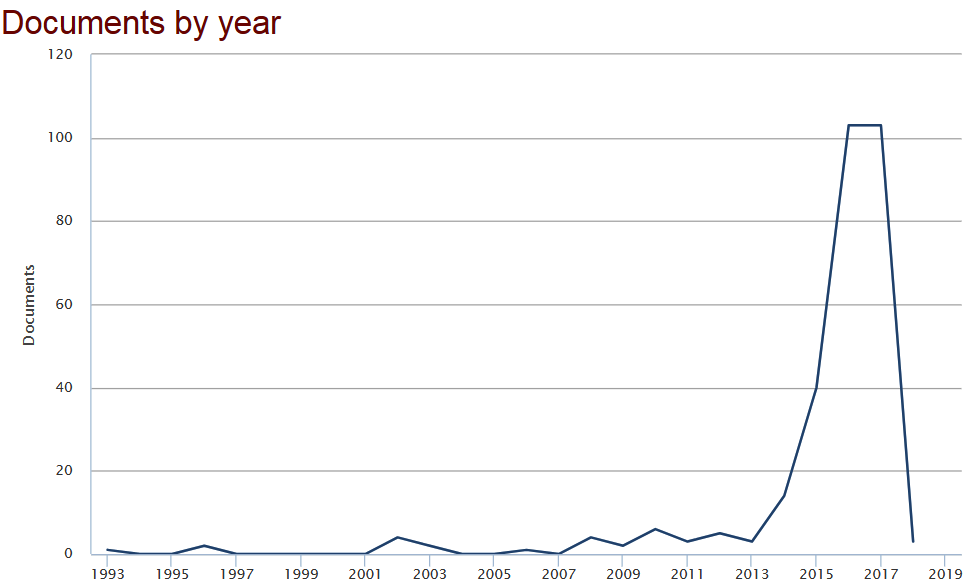
\includegraphics[scale=0.45]{figuras/papersbyyear.png}
\caption{Artigos por ano retornados pela \textit{string} de busca}
\label{fig:papersbyyear}
\end{figure}

\section{Condução da Revisão Sistemática da Literatura}\label{sec:crsl}
\subsection{Primeiro Filtro}
No primeiro filtro foi lido somente o título, resumo e as palavras-chaves do artigo.
A \textit{string} de busca retornou 281 artigos para classificar no primeiro filtro. Foram aceitos 99 (35\%) para o segundo filtro, 3 (1\%) duplicados e 179 (64\%) rejeitados.

Na Seção \ref{sec:stringdebusca}, o autor do protocolo esclarece porque utilizou os seguintes termos na \textit{string} de busca: "long short term memory", "LSTM”, "recurrent neural network" e "RNN", depois do primeiro filtro, realmente comprovou-se que estas técnicas são combinadas com as redes neurais de convolução para classificação de emoção em expressão facial, porém, somente em vídeos ou streaming de imagens. Portanto, os artigos retornados por essas palavras receberam a classificação de rejeitado devido a esta revisão focar em trabalhos com classificação em imagens estática sem streaming. 

\subsection{Segundo Filtro}
Para a realização do segundo filtro foi lido o artigo completo para a extração dos dados e, consequentemente a obtenção dos resultados. No segundo filtro tinham 99 artigos para classificar, onde 34 foram aceitos, 1 duplicados e 64 rejeitados.

\begin{figure}
\centering
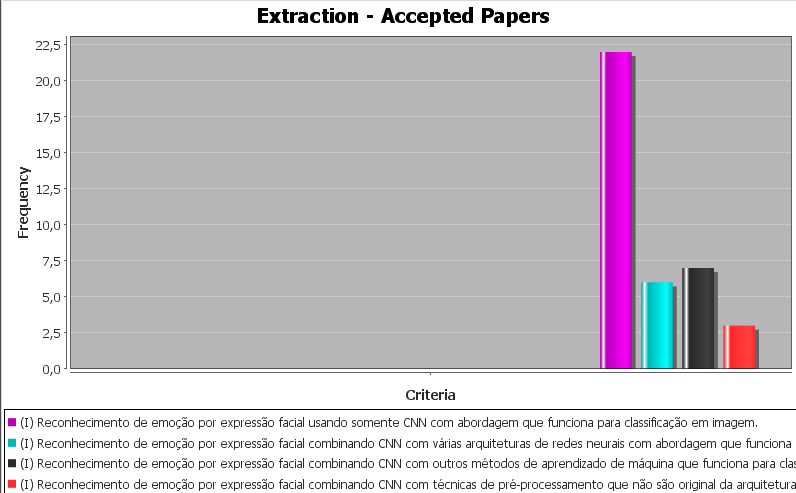
\includegraphics[scale=0.75]{figuras/paperscriteriaaccepted.png}
\caption{Gráfico representando a frequência dos critérios de inclusão para os artigos aceitos do segundo filtro}
\label{fig:papersbyyear}
\end{figure}

\begin{figure}
\centering
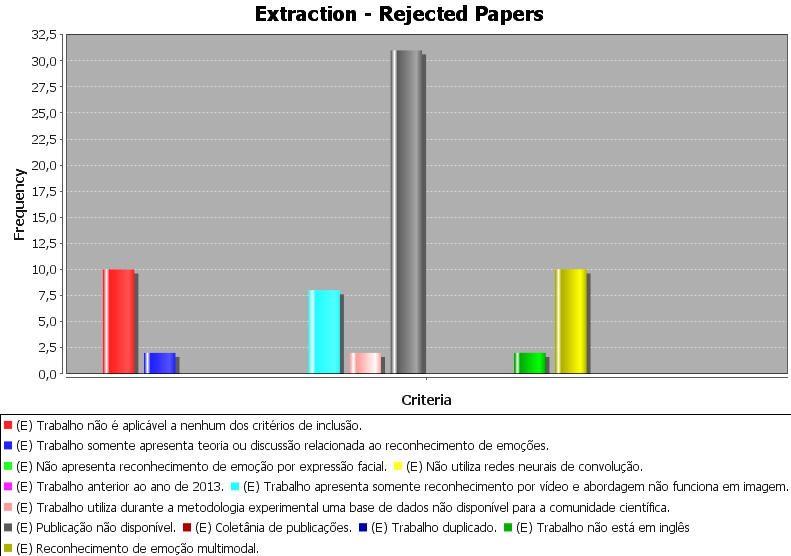
\includegraphics[scale=0.75]{figuras/paperscriteriarejected.png}
\caption{Gráfico representando a frequência dos critérios de exclusão para os artigos rejeitados do segundo filtro}
\label{fig:papersbyyear}
\end{figure}

\section{Resultados}\label{sec:results}
\subsection{Q1: Quais emoções têm sido reconhecidas por meio da expressão facial utilizando redes neurais de convolução?}
As emoções reconhecidas obviamente são as emoções que são representadas e contidas em base de dados, logo são as emoções básicas: neutralidade, felicidade, surpresa, tristeza, raiva, desgosto e medo. Alguns trabalhos como \cite{art8} reconhece também nojo.

\subsection{Q2: Quais tipos de pré-processamento tem sido realizado na imagem?}\label{sec:q2}
Abaixo segue uma lista com o pré-processamento e os trabalhos que fizeram utilização da técnica. 
\begin{itemize}
 \item \textbf{Detector de Face}: Consiste na detecção e recorte da face \citep{art1,art2,art6,art9,art12,art13,art15};
 \item \textbf{Normalização de Brilho (Equalização de histograma)}: Transformada para realce do contraste \citep{art2,art4,art6};
\item \textbf{Normalização Min e Max}: Transformação linear baseada no valor mínimo e máximo da imagem \citep{art4};
\item \textbf{Pontos da Face (pontos geométricos)}: Extração de pontos da face e a distância entre os pontos \citep{art11};
\item \textbf{Escala de Cinza}: Transformação da imagem para escala de cinza \citep{art12};
\item \textbf{Diferença Gaussiana}: Detecta as bordas do objeto, neste caso, evidencia as bordas da face \citep{art6};
\item \textbf{Filtro de Difusão Isotópica}: \citep{art6};
\item \textbf{Normalização DCT}: Transformada discreta do cosseno utilizada em compressão de dados e eventualmente evidenciando informações relevantes da imagem \citep{art6};
\item \textbf{Alinhamento da Face}: Utilização de uma rede neural \textit{autoencoder} para alinhar a face no centro \citep{art4}.
\end{itemize}

\subsection{Q3: Quais arquiteturas de redes neurais de convolução têm sido mais utilizadas?}
A Tabela \ref{arquiteturas} contém as arquiteturas encontradas e os trabalhos que a utilizaram, como podemos verificar a arquitetura AlexNet foi a mais utilizada.

\begin{table}[]\footnotesize
\centering
\begin{tabular}{|c|L|}
\hline
\textbf{Arquitetura} & \textbf{Trabalhos que utilizaram a arquitetura}                                                                                    \\ \hline
AlexNet              & \cite{art1}, \cite{art2}, \cite{art4}, \cite{art7}, \cite{art9}, \cite{art11}, \cite{art13}, \cite{art14}, \cite{art15} \\ \hline
GoogLeNet            & \cite{art10}                                                                                            \\ \hline
VGG                  & \cite{art8}, \cite{art13}                                                                                 \\ \hline
Ensemble             & \cite{art3}, \cite{art5}, \cite{art6}                                                                       \\ \hline
\end{tabular}

\caption{Principais arquiteturas de redes neurais de convolução e os trabalhos que utilizaram}
\label{arquiteturas}

\end{table}

\subsection{Q4: Quais técnicas, métodos e abordagens têm sido utilizados para tratar problemas na imagem como iluminação, rotação, obstrução e escala?}
A principal solução encontrada na literatura foi a ênfase na generalização adequada do aprendizado da rede neural de convolução, isto é, durante a fase de treinamento. Obviamente, as técnicas aplicadas no pré-processamento da imagem (ver Seção \ref{sec:q2}), contribuem para resolver problemas de iluminação por meio da equalização de histograma e de rotação com o alinhamento de face. Entretanto, um achado bastante interessante foi a utilização da técnica de aumento de dados, que consiste durante a fase de treinamento da rede neural de convolução em multiplicar por 10 vezes uma instância (imagem), isto é, gerando 10 novas imagens com pequenos giros da faces, e variações da rotação da pose, escala e iluminação. Acrescendo em 10 vezes o tamanho da base de treinamento, com inserção de variações da imagem resultando em melhor aprendizado da rede.

\subsection{Q5: Quais bases de dados têm sido utilizadas?}
Esta seção tem enfoque nas bases de dados mapeadas para reconhecimento de emoção por expressão facial em uma imagem estática.
Obviamente, é possível encontrar outras base de dados para reconhecimento de emoção que não seja 
por imagem estática, por exemplo, reconhecimento em vídeo, por sensores, em textos e outras.

As bases de dados para reconhecimento de emoção por expressão facial em uma imagem estática tem algo em comum, 
geralmente as amostras de expressões faciais são as mesmas emoções, as chamadas emoções básicas investigadas por \cite{ekman1994}
que são: neutralidade, felicidade, medo, desgosto, raiva, surpresa e tristeza, 
isto significa que são essas as emoções que a comunidade tem reconhecido por expressão facial.
As bases de dados mapeadas podem ser consultadas na Tabela \ref{database}.


\begin{table}\footnotesize
\centering

\begin{tabular}{|c|L|}
\hline
\textbf{Bases de Dados} & \multicolumn{1}{c|}{\textbf{Trabalhos que utilizaram a base para treinamento ou validação}}                                                                                                                  \\ \hline
CK+                    & \cite{art1}, \cite{art2}, \cite{art3}, \cite{art6}, \cite{art7}, \cite{art9}, \cite{art11}, \cite{art12}, \cite{art14}, \cite{art15} \\ \hline
JAFFE                  & \cite{art1}, \cite{art2}, \cite{art3}, \cite{art6}, \cite{art12}                                                                               \\ \hline
FER                    & \cite{art3}, \cite{art4}, \cite{art5}, \cite{art6}, \cite{art7}, \cite{art10}, \cite{art13}, \cite{art14}                                \\ \hline
FER+                   & \cite{art8}                                                                                                                                            \\ \hline
SFEW2.0                & \cite{art6}, \cite{art10}                                                                                                                            \\ \hline
KDEF                   & \cite{art6}                                                                                                                                            \\ \hline
MMI                    & \cite{art11}                                                                                                                                           \\ \hline
CIFE                   & \cite{art15}                                                                                                                                           \\ \hline
EmotiW2015             & \cite{art3}, \cite{art13}                                                                                                                            \\ \hline
\end{tabular}

\caption{Bases de Dados}

\label{table:database}
\end{table}



\subsection{Q6: Quais aplicações podem utilizar o reconhecimento de emoção por expressão facial?}
Há diversas aplicações para o reconhecimento de emoção no mundo real, foi percebido que os pesquisadores de reconhecimento de emoção por expressão facial utilizando rede neural de convolução, ultimamente concentraram seus esforços mais no desenvolvimento de reconhecedores de emoção do que a aplicação em cenários reais, mesmo assim, está aberto para trabalhos futuros inúmeras aplicações desses reconhecedores em diversas áreas, tendo destaque principalmente para: 

\begin{itemize}
\item \textbf{Interação humano computador}: no qual pode ser possível projetar interfaces que se adaptam ao estado emocional do usuário \citep{art1, art3, art5,art8};
\item \textbf{Psiquiatria e cuidados médicos}: 
no qual o reconhecedor de emoção deve monitorar constantemente o paciente ou usuário
fornecendo dados emocionais que podem contribuir para diagnósticos \citep{art1, art3, art12};
\item \textbf{Deficiente visual}: pois pessoas com alto grau de deficiência visual, tem dificuldades na
interação entre pessoas para identificar qual a emoção que as pessoas em volta estão emitindo \citep{art15},;
\item \textbf{Interação humano robô}: fazendo com que robôs estejam habilitados
a interagir com humanos podendo adaptar-se a emoção dos humanos em volta, 
ou até mesmo emitir emoção se aproximando de um humanoide \citep{art6, art14};
\item \textbf{Personagens virtuais e animação}: 
habilitando avatares a copiar expressão humana que podem ser útil para gravações de filmes de animação,
também pode ser usado em aplicações de animação como o popular aplicativo para \textit{smartphone} o \textit{Snapchat},
que identifica a expressão facial do usuário e retorna alguma animação sobrepondo a expressão anteriormente detectada do usuário \citep{art9, art11}.
\end{itemize}

\subsection{Questão Principal: Como reconhecer emoções por meio da expressão facial utilizando redes neurais de convolução em uma imagem estática?}
Diante das fichas de extração, foi percebido que a comunidade explorou diversas estratégias para processar imagens de expressão facial e reconhecer emoção. Algumas abordagens se destacam como: a técnica para aumentar os dados de treinamento e teste, utilizando a técnica flip fazendo até 10 pequenas rotações na imagem, para a CNN aprender a generalizar melhor sendo treinada e testada com uma base de dados maior. A técnica de normalização de brilho (equalização) no pré-processamento, no qual todos os trabalhos que utilizaram esta técnica aumentaram a acurácia do reconhecimento. Também merece destaque o trabalho de \cite{kim2016fusing} em que na sua abordagem, a rede de convolução recebe duas expressões faciais de entrada: a saída de um autoencoder que alinha a face e a imagem original sem alinhamento da face. Esta abordagem melhorou bastante o reconhecimento.

Com relação à arquitetura da rede neural de convolução, quem utilizou um SVM como classificador ao invés de um tradicional softmax obteve maior acurácia. Teve trabalhos que utilizou uma rede com camadas inceptions, hipergrafo, ensembles e concatenação de redes, e todas essas abordagens superaram uma CNN simples. Neste caso, falta um trabalho que possa dizer experimentalmente qual dessas arquiteturas é a melhor. 

Percebemos que existem várias bases de dados disponíveis para a comunidade. As bases de dados que foram mais exploradas foram a CK+, FER2013 e a JAFFE. A base CK+ é composta por expressões faciais capturadas em laboratório, por isso, tem altas taxas de reconhecimento, pois, sua dificuldade para o reconhecimento diminui. Já a base FER2013 foi capturada na “natureza”, por isso sua taxa de reconhecimento é mais baixa sendo uma base bastante complexa para classificação.

Notoriamente os trabalhos utilizam o algoritmo Viola Jones para detecção de face pelo programa OpenCV e fazem o recorte da face excluindo o background. Desta forma, elimina o trabalho da rede em aprender a separar o que é background e o que é face, diminuindo a complexidade da classificação.

Portanto, para reconhecer emoção em uma imagem estática, é necessário o treinamento de uma rede de convolução com um classificador na última camada, com a maior quantidade de dados possível, realizando o recorte da face e utilizar técnicas de normalização na imagem, ocasionando um aumento da taxa de reconhecimento. 

\section{Resumo}\label{sec:consfi}
Neste anexo apresentou uma revisão sistemática da literatura que investigou o estado-da-arte sobre o reconhecimento de emoção por expressão facial por meio de redes neurais de convolução. Verificamos que o tema está bem quente na comunidade, pois, antes de 2013 a String de busca retornou 33 artigos, e em 2013 (3 artigos), 2014 (14 artigos), 2015 (40 artigos), 2016 (103 artigos), 2017 (103 artigos) e 2018 (3 artigos), isso demonstra o crescimento exponencial da área.

Foram mapeadas as principais técnicas de pré-processamento, arquitetura de rede neural de convolução, base de dados, metodologias de treinamento e aplicações do reconhecimento de emoção. A impressão que fica é que a comunidade ainda não está utilizando esses classificadores no mundo real, e o amadurecimento rápido da área depois do surgimento do aprendizado profundo, nos levar acreditar que esses sistemas já estão prontos para ser posto em prática apoiando outras aplicações de interação humano computador, interação humano robô, educação, segurança, computação afetiva e etc.

\chapter{Resultados}\label{sec:results-anexos}

% Please add the following required packages to your document preamble:
% \usepackage{multirow}
\begin{table}[]
\centering
\caption{My caption}
\label{my-label}
\begin{tabular}{llcccc}
\hline
\textbf{Arquitetura}                    & \textbf{Emoção}       & \multicolumn{1}{l}{\textbf{Precisão}} & \multicolumn{1}{l}{\textbf{Revocação}} & \multicolumn{1}{l}{\textbf{F1-score}} & \multicolumn{1}{l}{\textbf{Acurácia}} \\ \hline
\multirow{8}{*}{Alexnet-13750}          & Raiva                 & 0.56                                  & 0.52                                   & 0.54                                  & \multirow{8}{*}{0.708}                \\
                                        & Desgosto              & 0.59                                  & 0.63                                   & 0.61                                  &                                       \\
                                        & Medo                  & 0.59                                  & 0.27                                   & 0.37                                  &                                       \\
                                        & Felicidade            & 0.82                                  & 0.89                                   & 0.85                                  &                                       \\
                                        & Tristeza              & 0.75                                  & 0.4                                    & 0.52                                  &                                       \\
                                        & Surpresa              & 0.81                                  & 0.8                                    & 0.81                                  &                                       \\
                                        & Neutralidade          & 0.55                                  & 0.74                                   & 0.63                                  &                                       \\
                                        & Média/Total           & 0.71                                  & 0.71                                   & 0.7                                   &                                       \\ \hline
\multirow{8}{*}{Alexnet-13800}          & Raiva                 & 0.56                                  & 0.52                                   & 0.54                                  & \multirow{8}{*}{0.704}                \\
                                        & Desgosto              & 0.69                                  & 0.53                                   & 0.6                                   &                                       \\
                                        & Medo                  & 0.43                                  & 0.42                                   & 0.42                                  &                                       \\
                                        & Felicidade            & 0.87                                  & 0.86                                   & 0.86                                  &                                       \\
                                        & Tristeza              & 0.54                                  & 0.6                                    & 0.57                                  &                                       \\
                                        & Surpresa              & 0.88                                  & 0.73                                   & 0.8                                   &                                       \\
                                        & Neutralidade          & 0.57                                  & 0.7                                    & 0.63                                  &                                       \\
                                        & Média/Total           & 0.72                                  & 0.7                                    & 0.71                                  &                                       \\ \hline
\multirow{8}{*}{Alexnet-16000}          & Raiva                 & 0.6                                   & 0.49                                   & 0.54                                  & \multirow{8}{*}{0.702}                \\
                                        & Desgosto              & 0.72                                  & 0.53                                   & 0.61                                  &                                       \\
                                        & Medo                  & 0.4                                   & 0.43                                   & 0.42                                  &                                       \\
                                        & Felicidade            & 0.84                                  & 0.89                                   & 0.86                                  &                                       \\
                                        & Tristeza              & 0.47                                  & 0.68                                   & 0.56                                  &                                       \\
                                        & Surpresa              & 0.79                                  & 0.81                                   & 0.8                                   &                                       \\
                                        & Neutralidade          & 0.69                                  & 0.52                                   & 0.59                                  &                                       \\
                                        & Média/Total           & 0.71                                  & 0.7                                    & 0.7                                   &                                       \\ \hline
\multirow{8}{*}{\textbf{Alexnet-17800}} & \textbf{Raiva}        & \textbf{0.51}                         & \textbf{0.6}                           & \textbf{0.55}                         & \multirow{8}{*}{\textbf{0.712}}       \\
                                        & \textbf{Desgosto}     & \textbf{0.62}                         & \textbf{0.64}                          & \textbf{0.63}                         &                                       \\
                                        & \textbf{Medo}         & \textbf{0.47}                         & \textbf{0.41}                          & \textbf{0.44}                         &                                       \\
                                        & \textbf{Felicidade}   & \textbf{0.84}                         & \textbf{0.89}                          & \textbf{0.86}                         &                                       \\
                                        & \textbf{Tristeza}     & \textbf{0.64}                         & \textbf{0.5}                           & \textbf{0.56}                         &                                       \\
                                        & \textbf{Surpresa}     & \textbf{0.84}                         & \textbf{0.77}                          & \textbf{0.8}                          &                                       \\
                                        & \textbf{Neutralidade} & \textbf{0.62}                         & \textbf{0.64}                          & \textbf{0.63}                         &                                       \\
                                        & \textbf{Média/Total}  & \textbf{0.71}                         & \textbf{0.71}                          & \textbf{0.71}                         &                                       \\ \hline
\multirow{8}{*}{Alexnet-18000}          & Raiva                 & 0.53                                  & 0.56                                   & 0.54                                  & \multirow{8}{*}{0.704}                \\
                                        & Desgosto              & 0.76                                  & 0.47                                   & 0.59                                  &                                       \\
                                        & Medo                  & 0.43                                  & 0.37                                   & 0.4                                   &                                       \\
                                        & Felicidade            & 0.82                                  & 0.89                                   & 0.85                                  &                                       \\
                                        & Tristeza              & 0.77                                  & 0.38                                   & 0.51                                  &                                       \\
                                        & Surpresa              & 0.74                                  & 0.84                                   & 0.79                                  &                                       \\
                                        & Neutralidade          & 0.58                                  & 0.69                                   & 0.63                                  &                                       \\
                                        & Média/Total           & 0.71                                  & 0.7                                    & 0.69                                  &                                       \\ \hline
\end{tabular}
\end{table}



% Please add the following required packages to your document preamble:
% \usepackage{multirow}
\begin{table}[]
\centering
\caption{My caption}
\label{my-label}
\begin{tabular}{llcccc}
\hline
\textbf{Arquitetura}                        & \textbf{Emoção}       & \multicolumn{1}{l}{\textbf{Precisão}} & \multicolumn{1}{l}{\textbf{Revocação}} & \multicolumn{1}{l}{\textbf{F1-score}} & \multicolumn{1}{l}{\textbf{Acurácia}} \\ \hline
\multirow{8}{*}{InceptionV3-25600}          & Raiva                 & 0.5                                   & 0.51                                   & 0.5                                   & \multirow{8}{*}{0.686}                \\
                                            & Desgosto              & 0.63                                  & 0.46                                   & 0.53                                  &                                       \\
                                            & Medo                  & 0.39                                  & 0.41                                   & 0.4                                   &                                       \\
                                            & Felicidade            & 0.86                                  & 0.9                                    & 0.88                                  &                                       \\
                                            & Tristeza              & 0.45                                  & 0.44                                   & 0.44                                  &                                       \\
                                            & Surpresa              & 0.82                                  & 0.79                                   & 0.8                                   &                                       \\
                                            & Neutralidade          & 0.58                                  & 0.6                                    & 0.59                                  &                                       \\
                                            & Média/Total           & 0.69                                  & 0.69                                   & 0.69                                  &                                       \\ \hline
\multirow{8}{*}{InceptionV3-26800}          & Raiva                 & 0.55                                  & 0.45                                   & 0.49                                  & \multirow{8}{*}{0.687}                \\
                                            & Desgosto              & 0.57                                  & 0.56                                   & 0.57                                  &                                       \\
                                            & Medo                  & 0.41                                  & 0.41                                   & 0.41                                  &                                       \\
                                            & Felicidade            & 0.91                                  & 0.85                                   & 0.88                                  &                                       \\
                                            & Tristeza              & 0.43                                  & 0.54                                   & 0.48                                  &                                       \\
                                            & Surpresa              & 0.85                                  & 0.78                                   & 0.81                                  &                                       \\
                                            & Neutralidade          & 0.56                                  & 0.66                                   & 0.6                                   &                                       \\
                                            & Média/Total           & 0.7                                   & 0.69                                   & 0.69                                  &                                       \\ \hline
\multirow{8}{*}{InceptionV3-28400}          & Raiva                 & 0.55                                  & 0.47                                   & 0.5                                   & \multirow{8}{*}{0.694}                \\
                                            & Desgosto              & 0.57                                  & 0.54                                   & 0.55                                  &                                       \\
                                            & Medo                  & 0.42                                  & 0.4                                    & 0.41                                  &                                       \\
                                            & Felicidade            & 0.87                                  & 0.9                                    & 0.88                                  &                                       \\
                                            & Tristeza              & 0.46                                  & 0.48                                   & 0.47                                  &                                       \\
                                            & Surpresa              & 0.85                                  & 0.78                                   & 0.81                                  &                                       \\
                                            & Neutralidade          & 0.58                                  & 0.63                                   & 0.6                                   &                                       \\
                                            & Média/Total           & 0.69                                  & 0.69                                   & 0.69                                  &                                       \\ \hline
\multirow{8}{*}{InceptionV3-30200}          & Raiva                 & 0.59                                  & 0.43                                   & 0.5                                   & \multirow{8}{*}{0.683}                \\
                                            & Desgosto              & 0.69                                  & 0.43                                   & 0.53                                  &                                       \\
                                            & Medo                  & 0.33                                  & 0.38                                   & 0.35                                  &                                       \\
                                            & Felicidade            & 0.89                                  & 0.87                                   & 0.88                                  &                                       \\
                                            & Tristeza              & 0.49                                  & 0.44                                   & 0.47                                  &                                       \\
                                            & Surpresa              & 0.72                                  & 0.85                                   & 0.78                                  &                                       \\
                                            & Neutralidade          & 0.56                                  & 0.64                                   & 0.6                                   &                                       \\
                                            & Média/Total           & 0.69                                  & 0.68                                   & 0.68                                  &                                       \\ \hline
\multirow{8}{*}{\textbf{InceptionV3-34000}} & \textbf{Raiva}        & \textbf{0.54}                         & \textbf{0.51}                          & \textbf{0.52}                         & \multirow{8}{*}{\textbf{0.701}}       \\
                                            & \textbf{Desgosto}     & \textbf{0.56}                         & \textbf{0.57}                          & \textbf{0.56}                         &                                       \\
                                            & \textbf{Medo}         & \textbf{0.47}                         & \textbf{0.42}                          & \textbf{0.44}                         &                                       \\
                                            & \textbf{Felicidade}   & \textbf{0.88}                         & \textbf{0.88}                          & \textbf{0.88}                         &                                       \\
                                            & \textbf{Tristeza}     & \textbf{0.47}                         & \textbf{0.53}                          & \textbf{0.5}                          &                                       \\
                                            & \textbf{Surpresa}     & \textbf{0.85}                         & \textbf{0.79}                          & \textbf{0.82}                         &                                       \\
                                            & \textbf{Neutralidade} & \textbf{0.59}                         & \textbf{0.62}                          & \textbf{0.61}                         &                                       \\
                                            & \textbf{Média/Total}  & \textbf{0.7}                          & \textbf{0.7}                           & \textbf{0.7}                          &                                       \\ \hline
\end{tabular}
\end{table}



% Please add the following required packages to your document preamble:
% \usepackage{multirow}
\begin{table}[]
\centering
\caption{My caption}
\label{my-label}
\begin{tabular}{llcccc}
\hline
\textbf{Arquitetura}                     & \textbf{Emoção}       & \multicolumn{1}{l}{\textbf{Precisão}} & \multicolumn{1}{l}{\textbf{Revocação}} & \multicolumn{1}{l}{\textbf{F1-score}} & \multicolumn{1}{l}{\textbf{Acurácia}} \\ \hline
\multirow{8}{*}{Resnet32-8600}           & Raiva                 & 0.64                                  & 0.65                                   & 0.64                                  & \multirow{8}{*}{0.753}                \\
                                         & Desgosto              & 0.73                                  & 0.63                                   & 0.68                                  &                                       \\
                                         & Medo                  & 0.46                                  & 0.52                                   & 0.49                                  &                                       \\
                                         & Felicidade            & 0.93                                  & 0.85                                   & 0.89                                  &                                       \\
                                         & Tristeza              & 0.73                                  & 0.58                                   & 0.65                                  &                                       \\
                                         & Surpresa              & 0.84                                  & 0.83                                   & 0.84                                  &                                       \\
                                         & Neutralidade          & 0.6                                   & 0.79                                   & 0.68                                  &                                       \\
                                         & Média/Total           & 0.77                                  & 0.75                                   & 0.76                                  &                                       \\ \hline
\multirow{8}{*}{Resnet32-9600}           & Raiva                 & 0.37                                  & 0.87                                   & 0.52                                  & \multirow{8}{*}{0.727}                \\
                                         & Desgosto              & 0.7                                   & 0.65                                   & 0.67                                  &                                       \\
                                         & Medo                  & 0.58                                  & 0.47                                   & 0.52                                  &                                       \\
                                         & Felicidade            & 0.91                                  & 0.87                                   & 0.89                                  &                                       \\
                                         & Tristeza              & 0.71                                  & 0.53                                   & 0.61                                  &                                       \\
                                         & Surpresa              & 0.82                                  & 0.82                                   & 0.82                                  &                                       \\
                                         & Neutralidade          & 0.77                                  & 0.55                                   & 0.64                                  &                                       \\
                                         & Média/Total           & 0.77                                  & 0.73                                   & 0.74                                  &                                       \\ \hline
\multirow{8}{*}{Resnet32-10625}          & Raiva                 & 0.8                                   & 0.51                                   & 0.62                                  & \multirow{8}{*}{0.75}                 \\
                                         & Desgosto              & 0.84                                  & 0.54                                   & 0.66                                  &                                       \\
                                         & Medo                  & 0.63                                  & 0.34                                   & 0.44                                  &                                       \\
                                         & Felicidade            & 0.89                                  & 0.9                                    & 0.89                                  &                                       \\
                                         & Tristeza              & 0.51                                  & 0.78                                   & 0.61                                  &                                       \\
                                         & Surpresa              & 0.75                                  & 0.88                                   & 0.81                                  &                                       \\
                                         & Neutralidade          & 0.69                                  & 0.66                                   & 0.68                                  &                                       \\
                                         & Média/Total           & 0.76                                  & 0.75                                   & 0.74                                  &                                       \\ \hline
\multirow{8}{*}{\textbf{Resnet32-11250}} & \textbf{Raiva}        & \textbf{0.69}                         & \textbf{0.57}                          & \textbf{0.62}                         & \multirow{8}{*}{\textbf{0.757}}       \\
                                         & \textbf{Desgosto}     & \textbf{0.79}                         & \textbf{0.66}                          & \textbf{0.72}                         &                                       \\
                                         & \textbf{Medo}         & \textbf{0.45}                         & \textbf{0.5}                           & \textbf{0.47}                         &                                       \\
                                         & \textbf{Felicidade}   & \textbf{0.9}                          & \textbf{0.89}                          & \textbf{0.9}                          &                                       \\
                                         & \textbf{Tristeza}     & \textbf{0.6}                          & \textbf{0.65}                          & \textbf{0.63}                         &                                       \\
                                         & \textbf{Surpresa}     & \textbf{0.82}                         & \textbf{0.86}                          & \textbf{0.84}                         &                                       \\
                                         & \textbf{Neutralidade} & \textbf{0.67}                         & \textbf{0.68}                          & \textbf{0.68}                         &                                       \\
                                         & \textbf{Média/Total}  & \textbf{0.76}                         & \textbf{0.76}                          & \textbf{0.76}                         &                                       \\ \hline
\multirow{8}{*}{Resnet32-14200}          & Raiva                 & 0.74                                  & 0.55                                   & 0.63                                  & \multirow{8}{*}{0.74}                 \\
                                         & Desgosto              & 0.86                                  & 0.52                                   & 0.65                                  &                                       \\
                                         & Medo                  & 0.56                                  & 0.48                                   & 0.52                                  &                                       \\
                                         & Felicidade            & 0.83                                  & 0.92                                   & 0.87                                  &                                       \\
                                         & Tristeza              & 0.61                                  & 0.69                                   & 0.65                                  &                                       \\
                                         & Surpresa              & 0.68                                  & 0.9                                    & 0.77                                  &                                       \\
                                         & Neutralidade          & 0.74                                  & 0.55                                   & 0.63                                  &                                       \\
                                         & Média/Total           & 0.74                                  & 0.74                                   & 0.73                                  &                                       \\ \hline
\end{tabular}
\end{table}


\chapter{Resultados Bases de Validação}\label{anex:results-anexos-val}

% Please add the following required packages to your document preamble:
% \usepackage{multirow}
\begin{table}[]
\centering
\caption{Resultados experimentais das redes neurais de convolução avaliando a base de validação CIFE-Test}
\label{table:cife-test}
\begin{tabular}{llcccc}
\hline
\textbf{Arquitetura}                   & \textbf{Emoção}       & \textbf{Precisão} & \textbf{Revocação} & \textbf{F1-score} & \textbf{Acurácia}               \\ \hline
\multirow{8}{*}{Alexnet}         & Raiva                 & 0.58              & 0.7                & 0.63              & \multirow{8}{*}{0.626}          \\
                                       & Desgosto              & 0.35              & 0.38               & 0.36              &                                 \\
                                       & Medo                  & 0.46              & 0.35               & 0.4               &                                 \\
                                       & Felicidade            & 0.72              & 0.8                & 0.76              &                                 \\
                                       & Tristeza              & 0.72              & 0.61               & 0.66              &                                 \\
                                       & Surpresa              & 0.73              & 0.62               & 0.67              &                                 \\
                                       & Neutralidade          & 0.5               & 0.51               & 0.5               &                                 \\
                                       & Média/Total           & 0.63              & 0.63               & 0.62              &                                 \\ \hline
\multirow{8}{*}{Inception-V3}     & Raiva                 & 0.62              & 0.62               & 0.62              & \multirow{8}{*}{0.613}          \\
                                       & Desgosto              & 0.26              & 0.3                & 0.28              &                                 \\
                                       & Medo                  & 0.47              & 0.46               & 0.46              &                                 \\
                                       & Felicidade            & 0.86              & 0.79               & 0.83              &                                 \\
                                       & Tristeza              & 0.56              & 0.54               & 0.55              &                                 \\
                                       & Surpresa              & 0.7               & 0.61               & 0.65              &                                 \\
                                       & Neutralidade          & 0.45              & 0.57               & 0.5               &                                 \\
                                       & Média/Total           & 0.63              & 0.61               & 0.62              &                                 \\ \hline
\multirow{8}{*}{\textbf{ResNet-34}} & \textbf{Raiva}        & \textbf{0.78}     & \textbf{0.6}       & \textbf{0.68}     & \multirow{8}{*}{\textbf{0.687}} \\
                                       & \textbf{Desgosto}     & \textbf{0.65}     & \textbf{0.34}      & \textbf{0.45}     &                                 \\
                                       & \textbf{Medo}         & \textbf{0.4}      & \textbf{0.42}      & \textbf{0.41}     &                                 \\
                                       & \textbf{Felicidade}   & \textbf{0.84}     & \textbf{0.87}      & \textbf{0.85}     &                                 \\
                                       & \textbf{Tristeza}     & \textbf{0.66}     & \textbf{0.71}      & \textbf{0.69}     &                                 \\
                                       & \textbf{Surpresa}     & \textbf{0.62}     & \textbf{0.81}      & \textbf{0.7}      &                                 \\
                                       & \textbf{Neutralidade} & \textbf{0.61}     & \textbf{0.6}       & \textbf{0.6}      &                                 \\
                                       & \textbf{Média/Total}  & \textbf{0.69}     & \textbf{0.69}      & \textbf{0.68}     &                                 \\ \hline
\end{tabular}
\end{table}


% Please add the following required packages to your document preamble:
% \usepackage{multirow}
\begin{table}[]
\centering
\caption{Resultados experimentais das redes neurais de convolução avaliando a base de validação CIFE-Train}
\label{table:cife-train}
\begin{tabular}{llcccc}
\hline
\textbf{Arquitetura}                   & \textbf{Emoção}       & \multicolumn{1}{l}{\textbf{Precisão}} & \multicolumn{1}{l}{\textbf{Revocação}} & \multicolumn{1}{l}{\textbf{F1-score}} & \multicolumn{1}{l}{\textbf{Acurácia}} \\ \hline
\multirow{8}{*}{Alexnet}         & Raiva                 & 0.55                                  & 0.6                                    & 0.58                                  & \multirow{8}{*}{0.624}                \\
                                       & Desgosto              & 0.3                                   & 0.31                                   & 0.3                                   &                                       \\
                                       & Medo                  & 0.5                                   & 0.49                                   & 0.5                                   &                                       \\
                                       & Felicidade            & 0.73                                  & 0.85                                   & 0.79                                  &                                       \\
                                       & Tristeza              & 0.68                                  & 0.6                                    & 0.64                                  &                                       \\
                                       & Surpresa              & 0.71                                  & 0.53                                   & 0.61                                  &                                       \\
                                       & Neutralidade          & 0.54                                  & 0.53                                   & 0.53                                  &                                       \\
                                       & Média/Total           & 0.62                                  & 0.62                                   & 0.62                                  &                                       \\ \hline
\multirow{8}{*}{Inception-V3}     & Raiva                 & 0.58                                  & 0.5                                    & 0.53                                  & \multirow{8}{*}{0.572}                \\
                                       & Desgosto              & 0.21                                  & 0.26                                   & 0.23                                  &                                       \\
                                       & Medo                  & 0.4                                   & 0.47                                   & 0.43                                  &                                       \\
                                       & Felicidade            & 0.83                                  & 0.79                                   & 0.81                                  &                                       \\
                                       & Tristeza              & 0.49                                  & 0.49                                   & 0.49                                  &                                       \\
                                       & Surpresa              & 0.69                                  & 0.54                                   & 0.61                                  &                                       \\
                                       & Neutralidade          & 0.44                                  & 0.53                                   & 0.48                                  &                                       \\
                                       & Média/Total           & 0.59                                  & 0.57                                   & 0.58                                  &                                       \\ \hline
\multirow{8}{*}{\textbf{ResNet-34}} & \textbf{Raiva}        & \textbf{0.71}                         & \textbf{0.61}                          & \textbf{0.66}                         & \multirow{8}{*}{\textbf{0.673}}       \\
                                       & \textbf{Desgosto}     & \textbf{0.44}                         & \textbf{0.22}                          & \textbf{0.3}                          &                                       \\
                                       & \textbf{Medo}         & \textbf{0.46}                         & \textbf{0.52}                          & \textbf{0.49}                         &                                       \\
                                       & \textbf{Felicidade}   & \textbf{0.82}                         & \textbf{0.83}                          & \textbf{0.83}                         &                                       \\
                                       & \textbf{Tristeza}     & \textbf{0.67}                         & \textbf{0.74}                          & \textbf{0.7}                          &                                       \\
                                       & \textbf{Surpresa}     & \textbf{0.6}                          & \textbf{0.75}                          & \textbf{0.67}                         &                                       \\
                                       & \textbf{Neutralidade} & \textbf{0.61}                         & \textbf{0.56}                          & \textbf{0.58}                         &                                       \\
                                       & \textbf{Média/Total}  & \textbf{0.67}                         & \textbf{0.67}                          & \textbf{0.67}                         &                                       \\ \hline
\end{tabular}
\end{table}



% Please add the following required packages to your document preamble:
% \usepackage{multirow}
\begin{table}[]
\centering
\caption{Resultados experimentais das redes neurais de convolução avaliando a base de validação CK}
\label{table:ck}
\begin{tabular}{llcccc}
\hline
\textbf{Arquitetura}                   & \textbf{Emoção}       & \multicolumn{1}{l}{\textbf{Precisão}} & \multicolumn{1}{l}{\textbf{Revocação}} & \multicolumn{1}{l}{\textbf{F1-score}} & \multicolumn{1}{l}{\textbf{Acurácia}} \\ \hline
\multirow{8}{*}{Alexnet}         & Raiva                 & 0.91                                  & 1                                      & 0.95                                  & \multirow{8}{*}{0.96}                 \\
                                       & Desgosto              & 0.98                                  & 0.97                                   & 0.98                                  &                                       \\
                                       & Medo                  & 0.89                                  & 0.96                                   & 0.92                                  &                                       \\
                                       & Felicidade            & 0.99                                  & 0.99                                   & 0.99                                  &                                       \\
                                       & Tristeza              & 0.98                                  & 0.84                                   & 0.91                                  &                                       \\
                                       & Surpresa              & 1                                     & 0.94                                   & 0.97                                  &                                       \\
                                       & Neutralidade          & 0                                     & 0                                      & 0                                     &                                       \\
                                       & Média/Total           & 0.97                                  & 0.96                                   & 0.96                                  &                                       \\ \hline
\multirow{8}{*}{Inception-V3}     & Raiva                 & 0.93                                  & 0.94                                   & 0.93                                  & \multirow{8}{*}{0.954}                \\
                                       & Desgosto              & 0.96                                  & 0.94                                   & 0.95                                  &                                       \\
                                       & Medo                  & 0.89                                  & 0.96                                   & 0.92                                  &                                       \\
                                       & Felicidade            & 0.99                                  & 0.98                                   & 0.99                                  &                                       \\
                                       & Tristeza              & 0.91                                  & 0.97                                   & 0.94                                  &                                       \\
                                       & Surpresa              & 1                                     & 0.94                                   & 0.97                                  &                                       \\
                                       & Neutralidade          & 0                                     & 0                                      & 0                                     &                                       \\
                                       & Média/Total           & 0.96                                  & 0.95                                   & 0.96                                  &                                       \\ \hline
\multirow{8}{*}{\textbf{ResNet-34}} & \textbf{Raiva}        & \textbf{0.97}                         & \textbf{0.96}                          & \textbf{0.97}                         & \multirow{8}{*}{\textbf{0.969}}       \\
                                       & \textbf{Desgosto}     & \textbf{1}                            & \textbf{0.92}                          & \textbf{0.96}                         &                                       \\
                                       & \textbf{Medo}         & \textbf{0.91}                         & \textbf{0.99}                          & \textbf{0.95}                         &                                       \\
                                       & \textbf{Felicidade}   & \textbf{0.98}                         & \textbf{0.99}                          & \textbf{0.99}                         &                                       \\
                                       & \textbf{Tristeza}     & \textbf{0.94}                         & \textbf{0.96}                          & \textbf{0.95}                         &                                       \\
                                       & \textbf{Surpresa}     & \textbf{0.98}                         & \textbf{0.99}                          & \textbf{0.99}                         &                                       \\
                                       & \textbf{Neutralidade} & \textbf{0}                            & \textbf{0}                             & \textbf{0}                            &                                       \\
                                       & \textbf{Média/Total}  & \textbf{0.97}                         & \textbf{0.97}                          & \textbf{0.97}                         &                                       \\ \hline
\end{tabular}
\end{table}


% Please add the following required packages to your document preamble:
% \usepackage{multirow}
\begin{table}[]
\centering
\caption{Resultados experimentais das redes neurais de convolução avaliando a base de validação FER}
\label{table:fer}
\begin{tabular}{llcccc}
\hline
\textbf{Arquitetura}                   & \textbf{Emoção}       & \multicolumn{1}{l}{\textbf{Precisão}} & \multicolumn{1}{l}{\textbf{Revocação}} & \multicolumn{1}{l}{\textbf{F1-score}} & \multicolumn{1}{l}{\textbf{Acurácia}} \\ \hline
\multirow{8}{*}{Alexnet}         & Raiva                 & 0.39                                  & 0.5                                    & 0.44                                  & \multirow{8}{*}{0.543}                \\
                                       & Desgosto              & 0.45                                  & 0.17                                   & 0.25                                  &                                       \\
                                       & Medo                  & 0.37                                  & 0.33                                   & 0.35                                  &                                       \\
                                       & Felicidade            & 0.74                                  & 0.79                                   & 0.76                                  &                                       \\
                                       & Tristeza              & 0.4                                   & 0.29                                   & 0.34                                  &                                       \\
                                       & Surpresa              & 0.72                                  & 0.64                                   & 0.67                                  &                                       \\
                                       & Neutralidade          & 0.49                                  & 0.52                                   & 0.51                                  &                                       \\
                                       & Média/Total           & 0.54                                  & 0.54                                   & 0.54                                  &                                       \\ \hline
\multirow{8}{*}{Inception-V3}     & Raiva                 & 0.43                                  & 0.4                                    & 0.41                                  & \multirow{8}{*}{0.529}                \\
                                       & Desgosto              & 0.13                                  & 0.25                                   & 0.17                                  &                                       \\
                                       & Medo                  & 0.39                                  & 0.36                                   & 0.37                                  &                                       \\
                                       & Felicidade            & 0.81                                  & 0.77                                   & 0.79                                  &                                       \\
                                       & Tristeza              & 0.29                                  & 0.38                                   & 0.32                                  &                                       \\
                                       & Surpresa              & 0.72                                  & 0.64                                   & 0.68                                  &                                       \\
                                       & Neutralidade          & 0.49                                  & 0.46                                   & 0.47                                  &                                       \\
                                       & Média/Total           & 0.55                                  & 0.53                                   & 0.54                                  &                                       \\ \hline
\multirow{8}{*}{\textbf{ResNet-34}} & \textbf{Raiva}        & \textbf{0.61}                         & \textbf{0.42}                          & \textbf{0.5}                          & \multirow{8}{*}{\textbf{0.604}}       \\
                                       & \textbf{Desgosto}     & \textbf{0.69}                         & \textbf{0.28}                          & \textbf{0.39}                         &                                       \\
                                       & \textbf{Medo}         & \textbf{0.35}                         & \textbf{0.47}                          & \textbf{0.4}                          &                                       \\
                                       & \textbf{Felicidade}   & \textbf{0.87}                         & \textbf{0.81}                          & \textbf{0.84}                         &                                       \\
                                       & \textbf{Tristeza}     & \textbf{0.41}                         & \textbf{0.42}                          & \textbf{0.41}                         &                                       \\
                                       & \textbf{Surpresa}     & \textbf{0.71}                         & \textbf{0.76}                          & \textbf{0.73}                         &                                       \\
                                       & \textbf{Neutralidade} & \textbf{0.56}                         & \textbf{0.61}                          & \textbf{0.58}                         &                                       \\
                                       & \textbf{Média/Total}  & \textbf{0.62}                         & \textbf{0.6}                           & \textbf{0.61}                         &                                       \\ \hline
\end{tabular}
\end{table}


% Please add the following required packages to your document preamble:
% \usepackage{multirow}
\begin{table}[]
\centering
\caption{Resultados experimentais das redes neurais de convolução avaliando a base de validação JAFFE}
\label{table:jaffe}
\begin{tabular}{llcccc}
\hline
\textbf{Arquitetura}                   & \textbf{Emoção}       & \multicolumn{1}{l}{\textbf{Precisão}} & \multicolumn{1}{l}{\textbf{Revocação}} & \multicolumn{1}{l}{\textbf{F1-score}} & \multicolumn{1}{l}{\textbf{Acurácia}} \\ \hline
\multirow{8}{*}{Alexnet}         & Raiva                 & 0.62                                  & 0.62                                   & 0.62                                  & \multirow{8}{*}{0.618}                \\
                                       & Desgosto              & 0.57                                  & 0.36                                   & 0.44                                  &                                       \\
                                       & Medo                  & 0                                     & 0                                      & 0                                     &                                       \\
                                       & Felicidade            & 0.93                                  & 0.93                                   & 0.93                                  &                                       \\
                                       & Tristeza              & 0.5                                   & 0.4                                    & 0.44                                  &                                       \\
                                       & Surpresa              & 0.67                                  & 0.8                                    & 0.73                                  &                                       \\
                                       & Neutralidade          & 0                                     & 0                                      & 0                                     &                                       \\
                                       & Média/Total           & 0.65                                  & 0.62                                   & 0.63                                  &                                       \\ \hline
\multirow{8}{*}{Inception-V3}     & Raiva                 & 0.45                                  & 0.62                                   & 0.53                                  & \multirow{8}{*}{0.636}                \\
                                       & Desgosto              & 0.6                                   & 0.27                                   & 0.37                                  &                                       \\
                                       & Medo                  & 0.5                                   & 0.5                                    & 0.5                                   &                                       \\
                                       & Felicidade            & 0.93                                  & 0.93                                   & 0.93                                  &                                       \\
                                       & Tristeza              & 0.44                                  & 0.4                                    & 0.42                                  &                                       \\
                                       & Surpresa              & 0.82                                  & 0.9                                    & 0.86                                  &                                       \\
                                       & Neutralidade          & 0                                     & 0                                      & 0                                     &                                       \\
                                       & Média/Total           & 0.67                                  & 0.64                                   & 0.64                                  &                                       \\ \hline
\multirow{8}{*}{\textbf{ResNet-34}} & \textbf{Raiva}        & \textbf{0.8}                          & \textbf{0.5}                           & \textbf{0.62}                         & \multirow{8}{*}{\textbf{0.654}}       \\
                                       & \textbf{Desgosto}     & \textbf{0.71}                         & \textbf{0.45}                          & \textbf{0.56}                         &                                       \\
                                       & \textbf{Medo}         & \textbf{1}                            & \textbf{0.5}                           & \textbf{0.67}                         &                                       \\
                                       & \textbf{Felicidade}   & \textbf{1}                            & \textbf{0.64}                          & \textbf{0.78}                         &                                       \\
                                       & \textbf{Tristeza}     & \textbf{0.58}                         & \textbf{0.7}                           & \textbf{0.64}                         &                                       \\
                                       & \textbf{Surpresa}     & \textbf{0.53}                         & \textbf{1}                             & \textbf{0.69}                         &                                       \\
                                       & \textbf{Neutralidade} & \textbf{0}                            & \textbf{0}                             & \textbf{0}                            &                                       \\
                                       & \textbf{Média/Total}  & \textbf{0.75}                         & \textbf{0.65}                          & \textbf{0.67}                         &                                       \\ \hline
\end{tabular}
\end{table}



% Please add the following required packages to your document preamble:
% \usepackage{multirow}
\begin{table}[]
\centering
\caption{Resultados experimentais das redes neurais de convolução avaliando a base de validação KDEF}
\label{table:kdef}
\begin{tabular}{llcccc}
\hline
\textbf{Arquitetura}                   & \textbf{Emoção}       & \multicolumn{1}{l}{\textbf{Precisão}} & \multicolumn{1}{l}{\textbf{Revocação}} & \multicolumn{1}{l}{\textbf{F1-score}} & \multicolumn{1}{l}{\textbf{Acurácia}} \\ \hline
\multirow{8}{*}{Alexnet}         & Raiva                 & 0.65                                  & 0.59                                   & 0.62                                  & \multirow{8}{*}{0.624}                \\
                                       & Desgosto              & 0.6                                   & 0.79                                   & 0.68                                  &                                       \\
                                       & Medo                  & 0.48                                  & 0.43                                   & 0.45                                  &                                       \\
                                       & Felicidade            & 0.8                                   & 0.93                                   & 0.86                                  &                                       \\
                                       & Tristeza              & 0.52                                  & 0.4                                    & 0.45                                  &                                       \\
                                       & Surpresa              & 0.81                                  & 0.61                                   & 0.7                                   &                                       \\
                                       & Neutralidade          & 0.52                                  & 0.62                                   & 0.57                                  &                                       \\
                                       & Média/Total           & 0.63                                  & 0.62                                   & 0.62                                  &                                       \\ \hline
\multirow{8}{*}{Inception-V3}     & Raiva                 & 0.51                                  & 0.53                                   & 0.52                                  & \multirow{8}{*}{0.587}                \\
                                       & Desgosto              & 0.62                                  & 0.45                                   & 0.52                                  &                                       \\
                                       & Medo                  & 0.54                                  & 0.36                                   & 0.43                                  &                                       \\
                                       & Felicidade            & 0.93                                  & 0.87                                   & 0.9                                   &                                       \\
                                       & Tristeza              & 0.34                                  & 0.5                                    & 0.41                                  &                                       \\
                                       & Surpresa              & 0.76                                  & 0.8                                    & 0.78                                  &                                       \\
                                       & Neutralidade          & 0.54                                  & 0.6                                    & 0.57                                  &                                       \\
                                       & Média/Total           & 0.61                                  & 0.59                                   & 0.59                                  &                                       \\ \hline
\multirow{8}{*}{\textbf{ResNet-34}} & \textbf{Raiva}        & \textbf{0.7}                          & \textbf{0.7}                           & \textbf{0.7}                          & \multirow{8}{*}{\textbf{0.751}}       \\
                                       & \textbf{Desgosto}     & \textbf{0.65}                         & \textbf{0.88}                          & \textbf{0.75}                         &                                       \\
                                       & \textbf{Medo}         & \textbf{0.73}                         & \textbf{0.44}                          & \textbf{0.55}                         &                                       \\
                                       & \textbf{Felicidade}   & \textbf{0.94}                         & \textbf{0.99}                          & \textbf{0.96}                         &                                       \\
                                       & \textbf{Tristeza}     & \textbf{0.69}                         & \textbf{0.7}                           & \textbf{0.7}                          &                                       \\
                                       & \textbf{Surpresa}     & \textbf{0.73}                         & \textbf{0.9}                           & \textbf{0.8}                          &                                       \\
                                       & \textbf{Neutralidade} & \textbf{0.86}                         & \textbf{0.66}                          & \textbf{0.75}                         &                                       \\
                                       & \textbf{Média/Total}  & \textbf{0.76}                         & \textbf{0.75}                          & \textbf{0.74}                         &                                       \\ \hline
\end{tabular}
\end{table}


% Please add the following required packages to your document preamble:
% \usepackage{multirow}
\begin{table}[]
\centering
\caption{Resultados experimentais das redes neurais de convolução avaliando a base de validação NovaEmotions}
\label{table:novaemotions}
\begin{tabular}{llcccc}
\hline
\textbf{Arquitetura}                   & \textbf{Emoção}       & \multicolumn{1}{l}{\textbf{Precisão}} & \multicolumn{1}{l}{\textbf{Revocação}} & \multicolumn{1}{l}{\textbf{F1-score}} & \multicolumn{1}{l}{\textbf{Acurácia}}   \\ \hline
\multirow{8}{*}{Alexnet}         & Raiva                 & 0.68                         & 0.33                          & 0.44                         & \multirow{8}{*}{0.857}         \\
                                       & Desgosto              & 0.69                         & 0.63                          & 0.66                         &                                \\
                                       & Medo                  & 0.57                         & 0.25                          & 0.34                         &                                \\
                                       & Felicidade            & 0.89                         & 0.94                          & 0.92                         &                                \\
                                       & Tristeza              & 0.86                         & 0.73                          & 0.79                         &                                \\
                                       & Surpresa              & 0.9                          & 0.87                          & 0.89                         &                                \\
                                       & Neutralidade          & 0.76                         & 0.77                          & 0.76                         &                                \\
                                       & Média/Total           & 0.85                         & 0.86                          & 0.85                         &                                \\ \hline
\multirow{8}{*}{Inception-V3}     & Raiva                 & 0.3                          & 0.22                          & 0.25                         & \multirow{8}{*}{0.853}         \\
                                       & Desgosto              & 0.68                         & 0.6                           & 0.64                         &                                \\
                                       & Medo                  & 0.44                         & 0.15                          & 0.23                         &                                \\
                                       & Felicidade            & 0.9                          & 0.94                          & 0.92                         &                                \\
                                       & Tristeza              & 0.89                         & 0.67                          & 0.77                         &                                \\
                                       & Surpresa              & 0.92                         & 0.88                          & 0.9                          &                                \\
                                       & Neutralidade          & 0.71                         & 0.77                          & 0.74                         &                                \\
                                       & Média/Total           & 0.85                         & 0.85                          & 0.85                         &                                \\ \hline
\multirow{8}{*}{\textbf{ResNet-34}} & \textbf{Raiva}        & \textbf{0.54}                & \textbf{0.33}                 & \textbf{0.41}                & \multirow{8}{*}{\textbf{0.87}} \\
                                       & \textbf{Desgosto}     & \textbf{0.85}                & \textbf{0.65}                 & \textbf{0.74}                &                                \\
                                       & \textbf{Medo}         & \textbf{0.73}                & \textbf{0.15}                 & \textbf{0.25}                &                                \\
                                       & \textbf{Felicidade}   & \textbf{0.93}                & \textbf{0.93}                 & \textbf{0.93}                &                                \\
                                       & \textbf{Tristeza}     & \textbf{0.71}                & \textbf{0.88}                 & \textbf{0.78}                &                                \\
                                       & \textbf{Surpresa}     & \textbf{0.93}                & \textbf{0.89}                 & \textbf{0.91}                &                                \\
                                       & \textbf{Neutralidade} & \textbf{0.75}                & \textbf{0.79}                 & \textbf{0.77}                &                                \\
                                       & \textbf{Média/Total}  & \textbf{0.87}                & \textbf{0.87}                 & \textbf{0.87}                &                                \\ \hline
\end{tabular}
\end{table}


% Please add the following required packages to your document preamble:
% \usepackage{multirow}
\begin{table}[]
\centering
\caption{Resultados experimentais das redes neurais de convolução avaliando a base de validação RAFD}
\label{table:rafd}
\begin{tabular}{llcccc}
\hline
\textbf{Arquitetura}                   & \textbf{Emoção}       & \multicolumn{1}{l}{\textbf{Precisão}} & \multicolumn{1}{l}{\textbf{Revocação}} & \multicolumn{1}{l}{\textbf{F1-score}} & \multicolumn{1}{l}{\textbf{Acurácia}} \\ \hline
\multirow{8}{*}{Alexnet}         & Raiva                 & 0.66                                  & 0.77                                   & 0.71                                  & \multirow{8}{*}{0.641}                \\
                                       & Desgosto              & 0.58                                  & 0.75                                   & 0.66                                  &                                       \\
                                       & Medo                  & 0.74                                  & 0.58                                   & 0.65                                  &                                       \\
                                       & Felicidade            & 0.72                                  & 0.81                                   & 0.76                                  &                                       \\
                                       & Tristeza              & 0.67                                  & 0.36                                   & 0.47                                  &                                       \\
                                       & Surpresa              & 0.76                                  & 0.73                                   & 0.74                                  &                                       \\
                                       & Neutralidade          & 0.45                                  & 0.38                                   & 0.41                                  &                                       \\
                                       & Média/Total           & 0.65                                  & 0.64                                   & 0.63                                  &                                       \\ \hline
\multirow{8}{*}{Inception-V3}     & Raiva                 & 0.65                                  & 0.72                                   & 0.68                                  & \multirow{8}{*}{0.674}                \\
                                       & Desgosto              & 0.71                                  & 0.65                                   & 0.68                                  &                                       \\
                                       & Medo                  & 0.82                                  & 0.55                                   & 0.66                                  &                                       \\
                                       & Felicidade            & 0.89                                  & 0.87                                   & 0.88                                  &                                       \\
                                       & Tristeza              & 0.46                                  & 0.68                                   & 0.55                                  &                                       \\
                                       & Surpresa              & 0.82                                  & 0.81                                   & 0.81                                  &                                       \\
                                       & Neutralidade          & 0.49                                  & 0.48                                   & 0.49                                  &                                       \\
                                       & Média/Total           & 0.69                                  & 0.67                                   & 0.68                                  &                                       \\ \hline
\multirow{8}{*}{\textbf{ResNet-34}} & \textbf{Raiva}        & \textbf{0.67}                         & \textbf{0.92}                          & \textbf{0.77}                         & \multirow{8}{*}{\textbf{0.775}}       \\
                                       & \textbf{Desgosto}     & \textbf{0.8}                          & \textbf{0.81}                          & \textbf{0.81}                         &                                       \\
                                       & \textbf{Medo}         & \textbf{0.81}                         & \textbf{0.65}                          & \textbf{0.72}                         &                                       \\
                                       & \textbf{Felicidade}   & \textbf{0.87}                         & \textbf{0.94}                          & \textbf{0.9}                          &                                       \\
                                       & \textbf{Tristeza}     & \textbf{0.74}                         & \textbf{0.7}                           & \textbf{0.72}                         &                                       \\
                                       & \textbf{Surpresa}     & \textbf{0.76}                         & \textbf{0.94}                          & \textbf{0.84}                         &                                       \\
                                       & \textbf{Neutralidade} & \textbf{0.8}                          & \textbf{0.44}                          & \textbf{0.57}                         &                                       \\
                                       & \textbf{Média/Total}  & \textbf{0.78}                         & \textbf{0.78}                          & \textbf{0.77}                         &                                       \\ \hline
\end{tabular}
\end{table}

\end{anexosenv}

%
%\input{files}

%---------------------------------------------------------------------
% INDICE REMISSIVO
%---------------------------------------------------------------------

\printindex

\end{document}
